\appendix
\renewcommand{\thechapter}{B}
\renewcommand{\chaptername}{Appendix}

\chapter{Experimental and FDS Data Plots}
\label{chap:exp_FDS_plots}

\section{Temperature}
\subsection*{\textit{Hot Gas Layer Temperatures}}
\begin{figure}[!h]
	\centering
	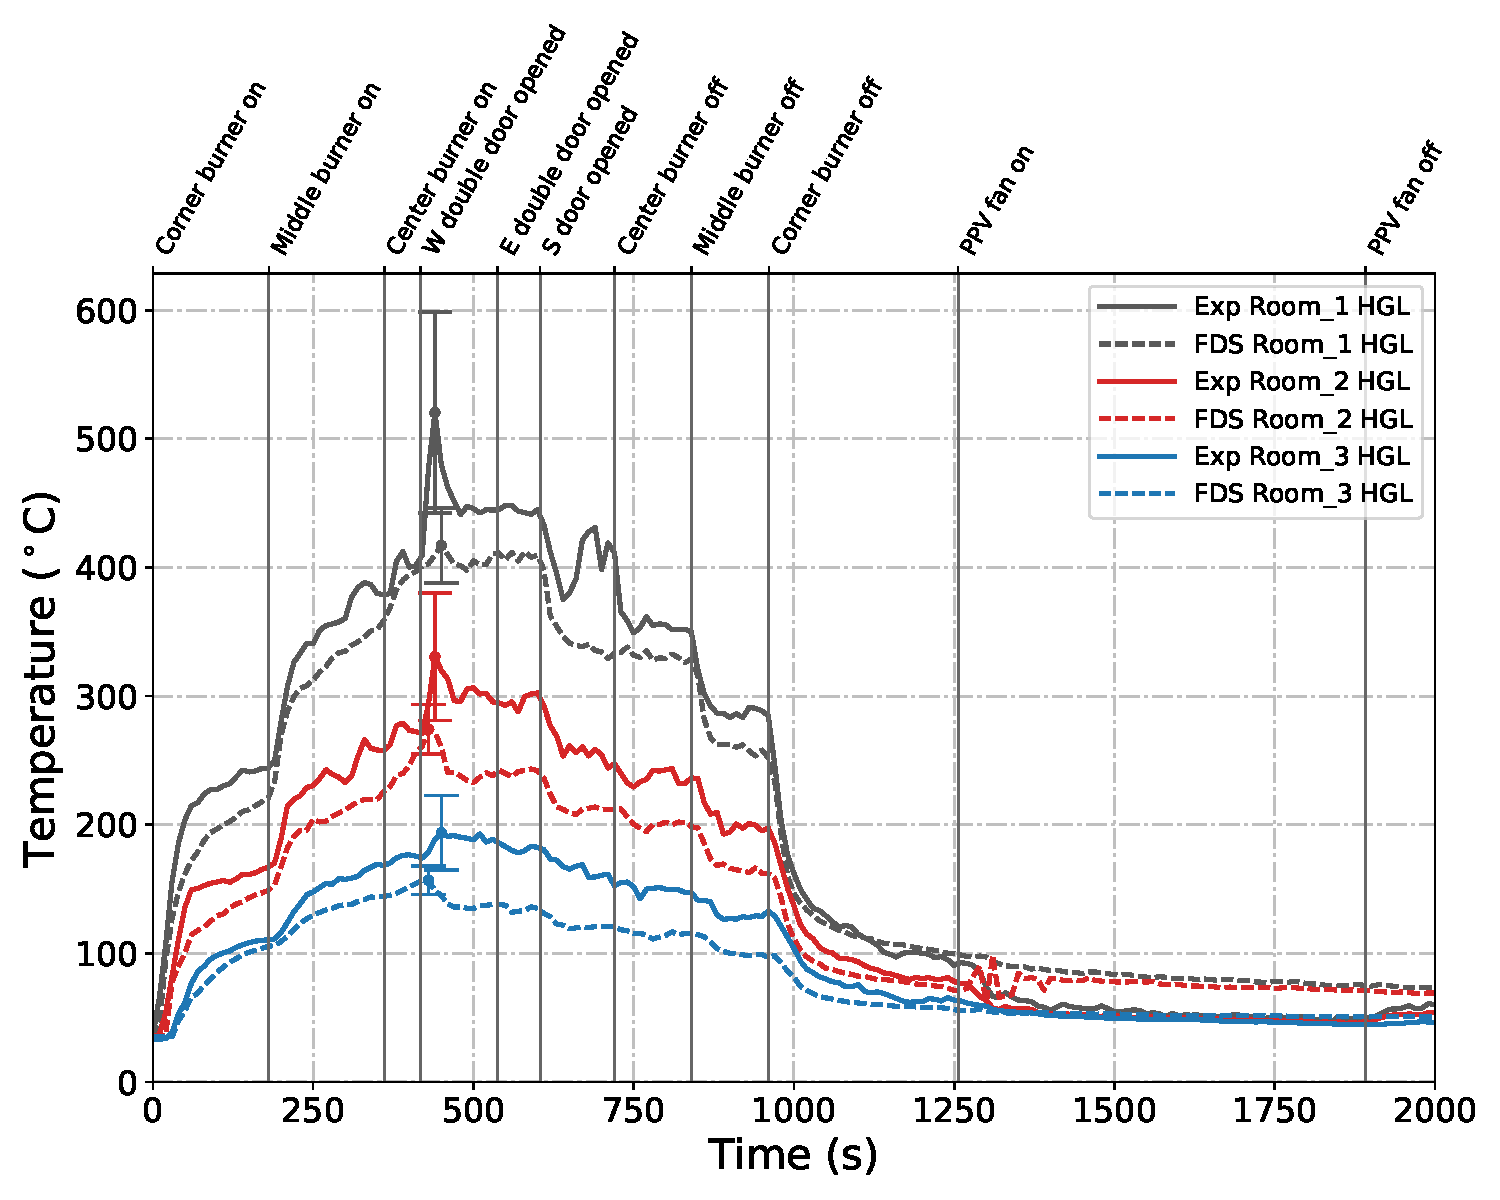
\includegraphics[width=\columnwidth]{Figures/Plots/Validation/Temperature/Test_2_HGL}
	\caption[Plots of measured and predicted hot gas layer temperatures during Test~2.]{Plots of measured and predicted hot gas layer temperatures in the three rooms of the East Structure during Test~2.}
	\label{fig:HGL_data_Test2}
\end{figure}

\begin{figure}[!h]
	\centering
	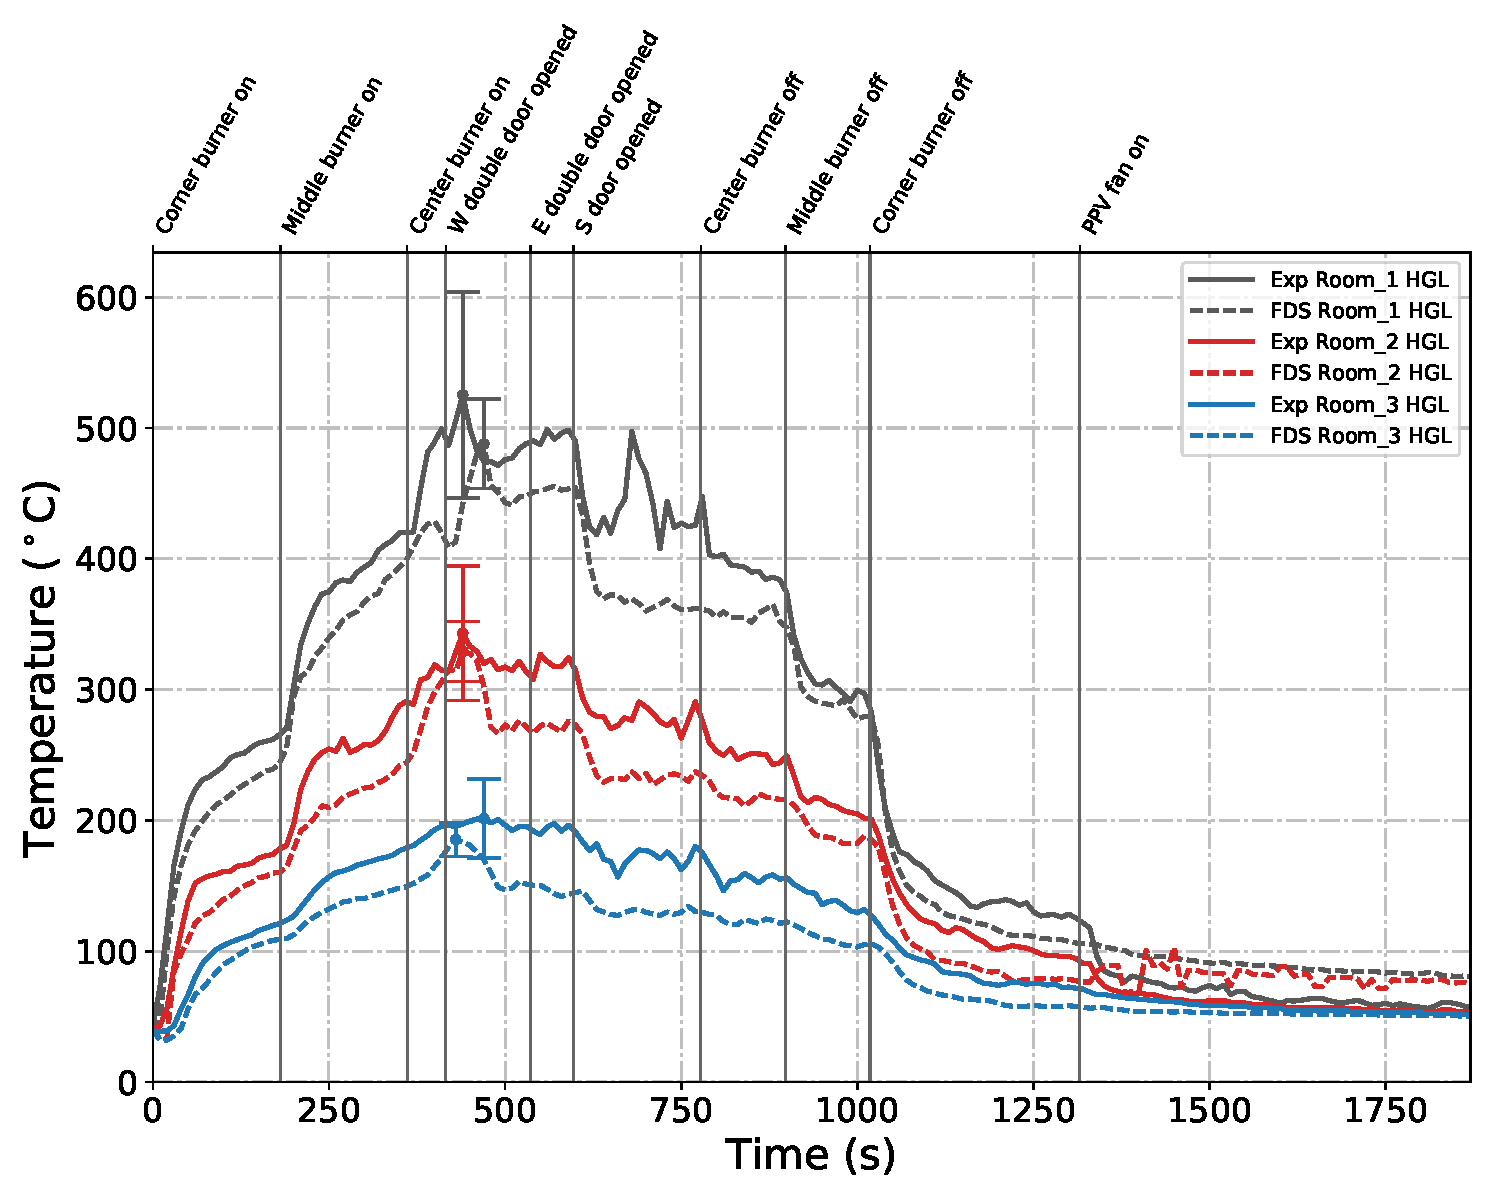
\includegraphics[width=\columnwidth]{Figures/Plots/Validation/Temperature/Test_3_HGL}
	\caption[Plots of measured and predicted hot gas layer temperatures during Test~3.]{Plots of measured and predicted hot gas layer temperatures in the three rooms of the East Structure during Test~3.}
	\label{fig:HGL_data_Test3}
\end{figure}

\begin{figure}[!h]
	\centering
	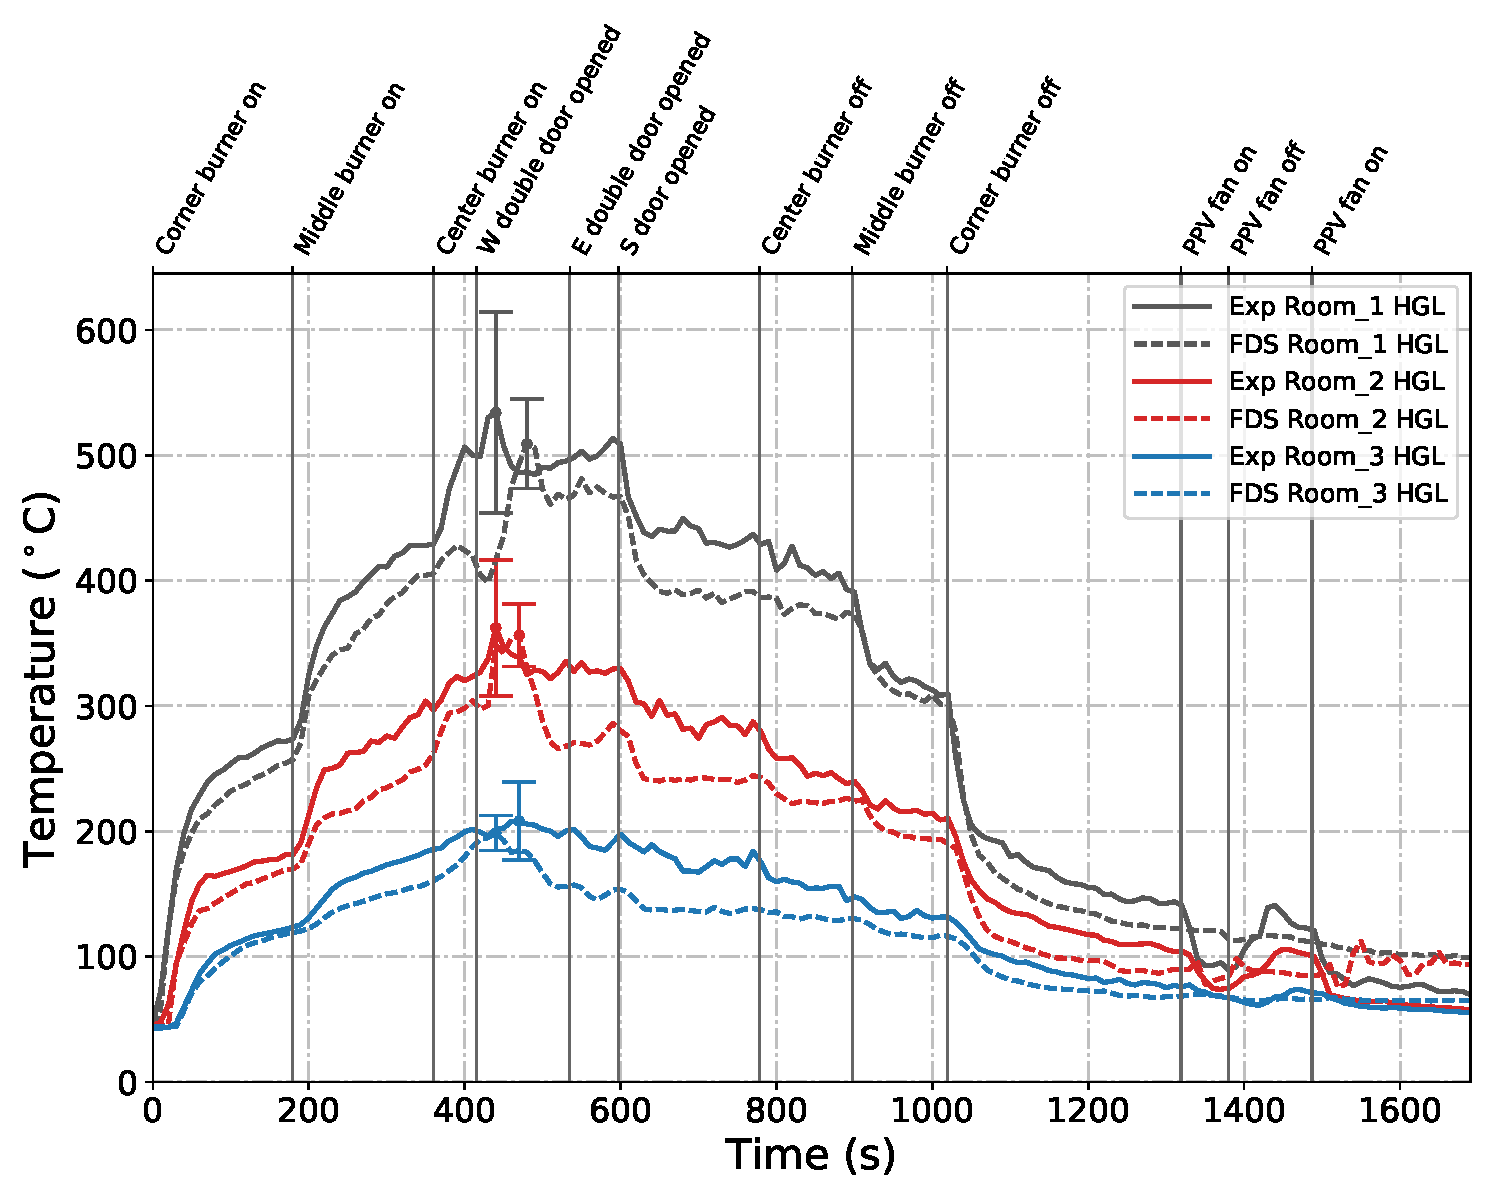
\includegraphics[width=\columnwidth]{Figures/Plots/Validation/Temperature/Test_4_HGL}
	\caption[Plots of measured and predicted hot gas layer temperatures during Test~4.]{Plots of measured and predicted hot gas layer temperatures in the three rooms of the East Structure during Test~4.}
	\label{fig:HGL_data_Test4}
\end{figure}

\begin{figure}[!h]
	\centering
	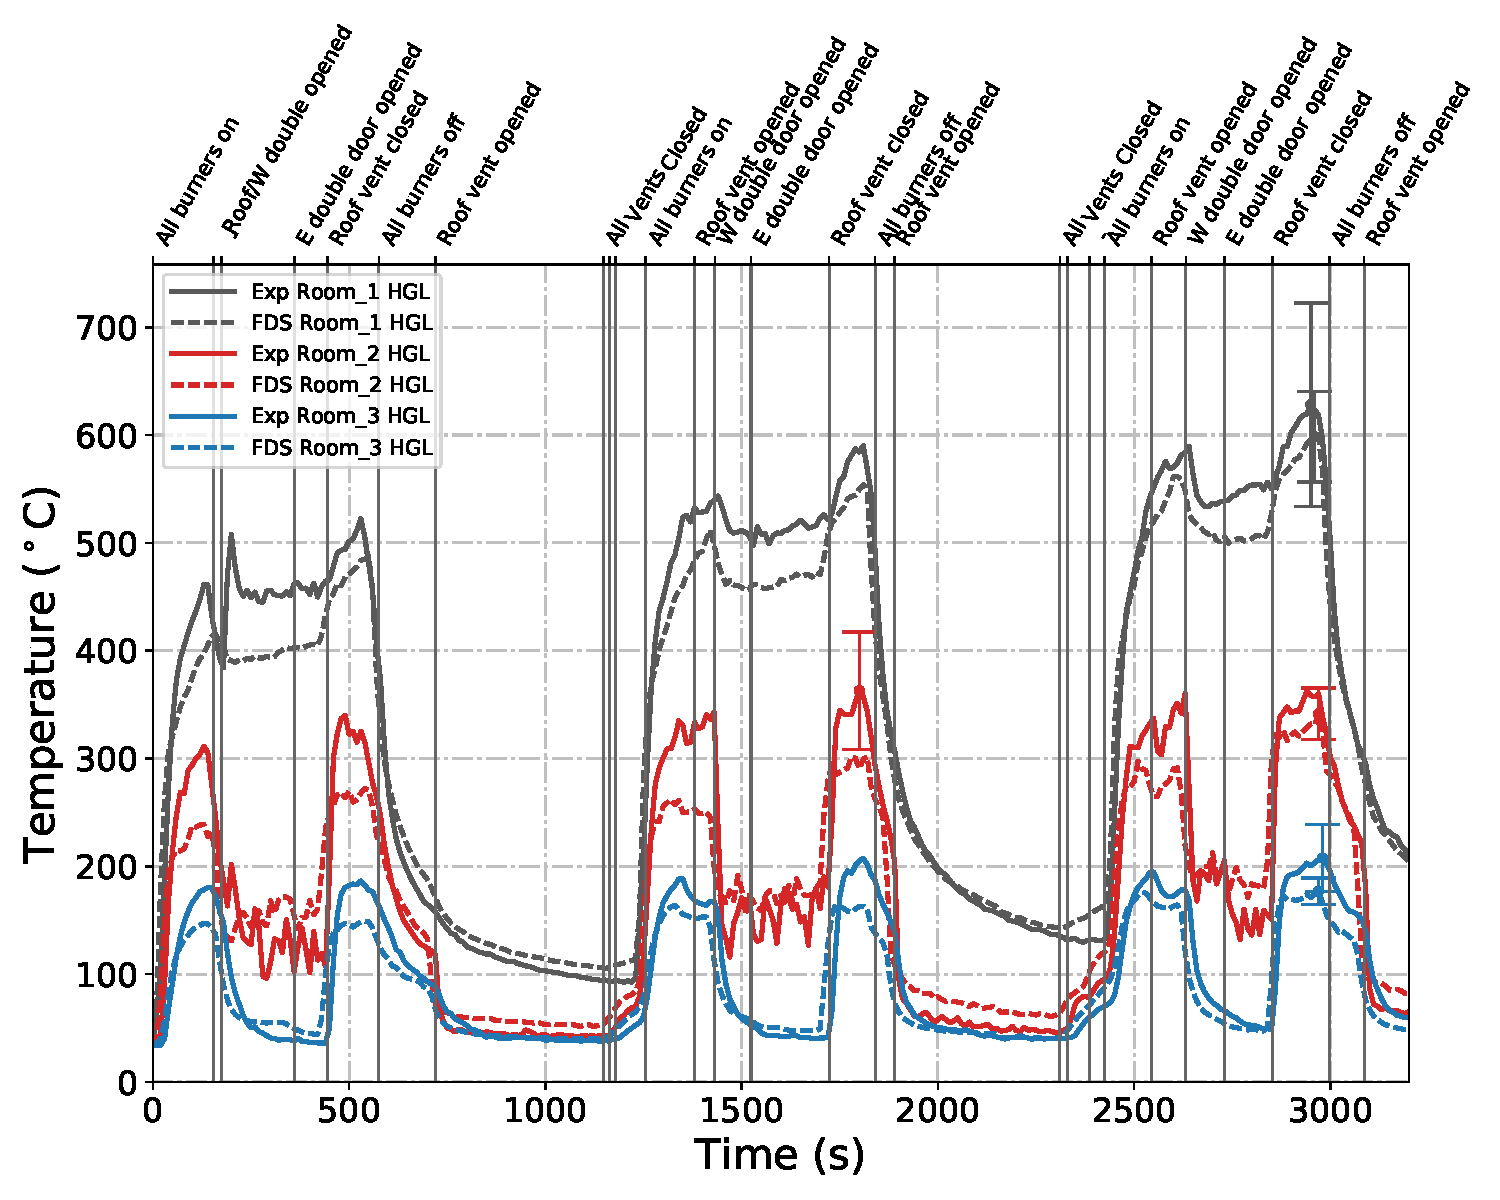
\includegraphics[width=\columnwidth]{Figures/Plots/Validation/Temperature/Test_5_HGL}
	\caption[Plots of measured and predicted hot gas layer temperatures during Test~5.]{Plots of measured and predicted hot gas layer temperatures in the three rooms of the East Structure during Test~5.}
	\label{fig:HGL_data_Test5}
\end{figure}

\begin{figure}[!h]
	\centering
	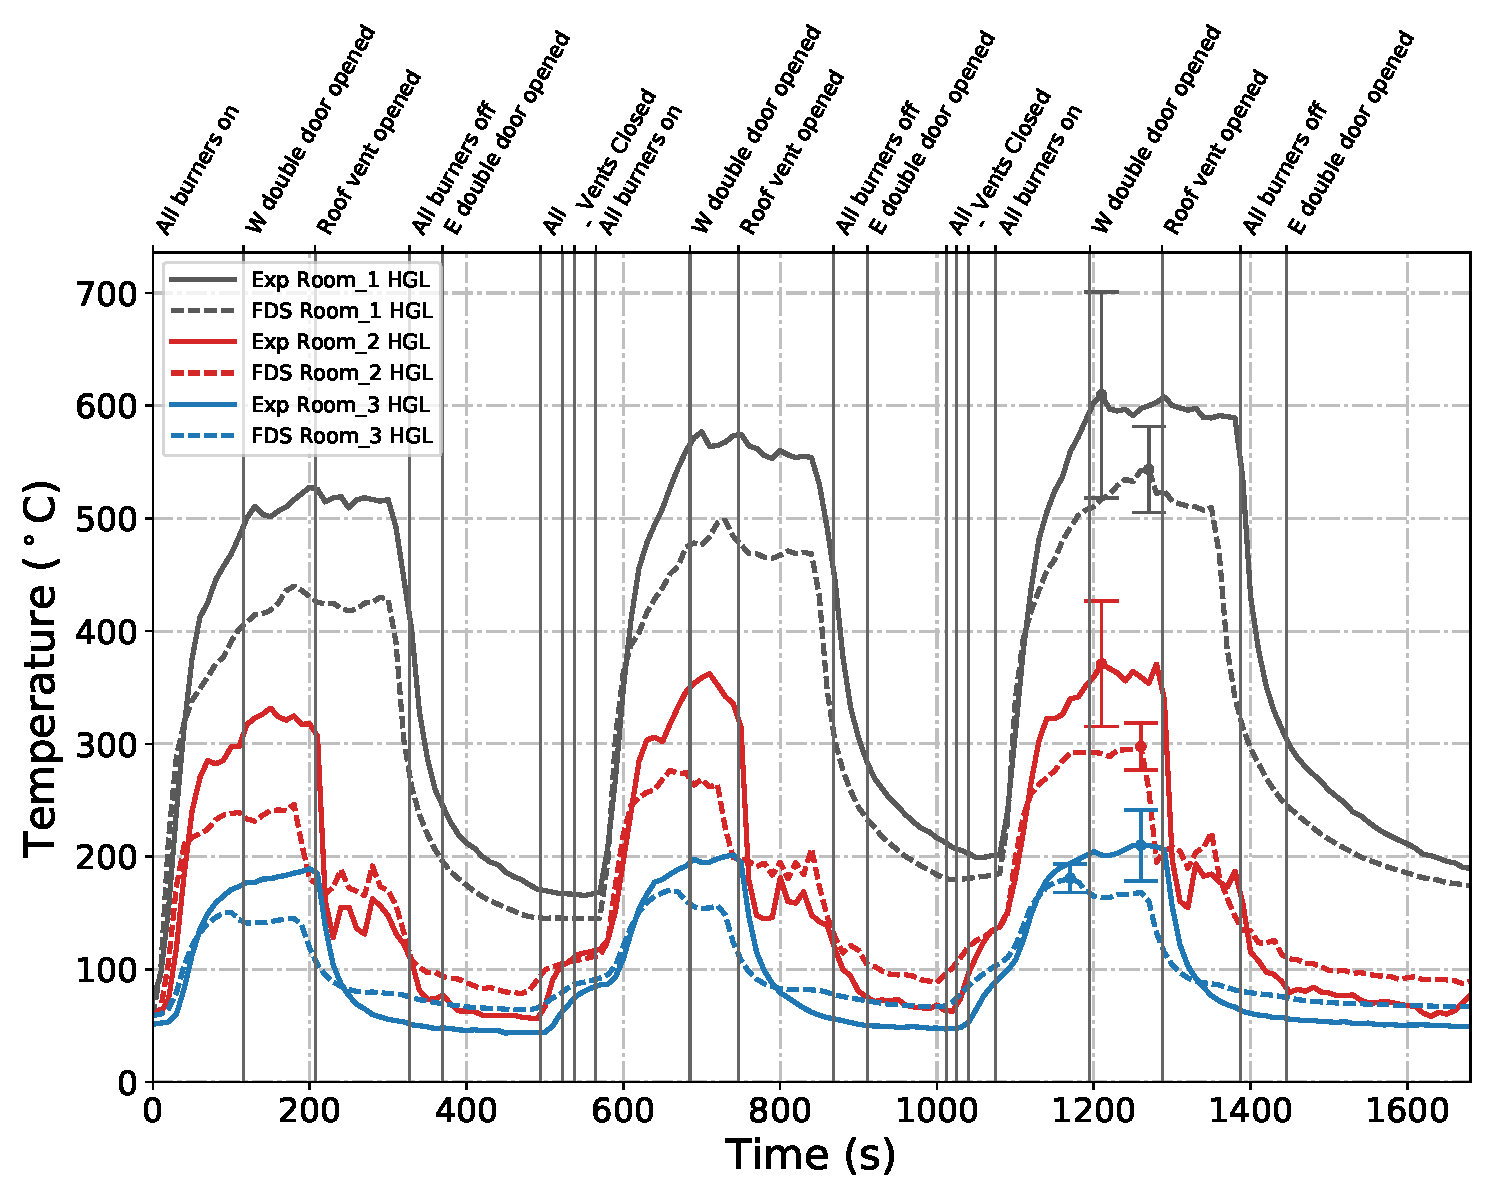
\includegraphics[width=\columnwidth]{Figures/Plots/Validation/Temperature/Test_6_HGL}
	\caption[Plots of measured and predicted hot gas layer temperatures during Test~6.]{Plots of measured and predicted hot gas layer temperatures in the three rooms of the East Structure during Test~6.}
	\label{fig:HGL_data_Test6}
\end{figure}

\begin{figure}[!h]
	\centering
	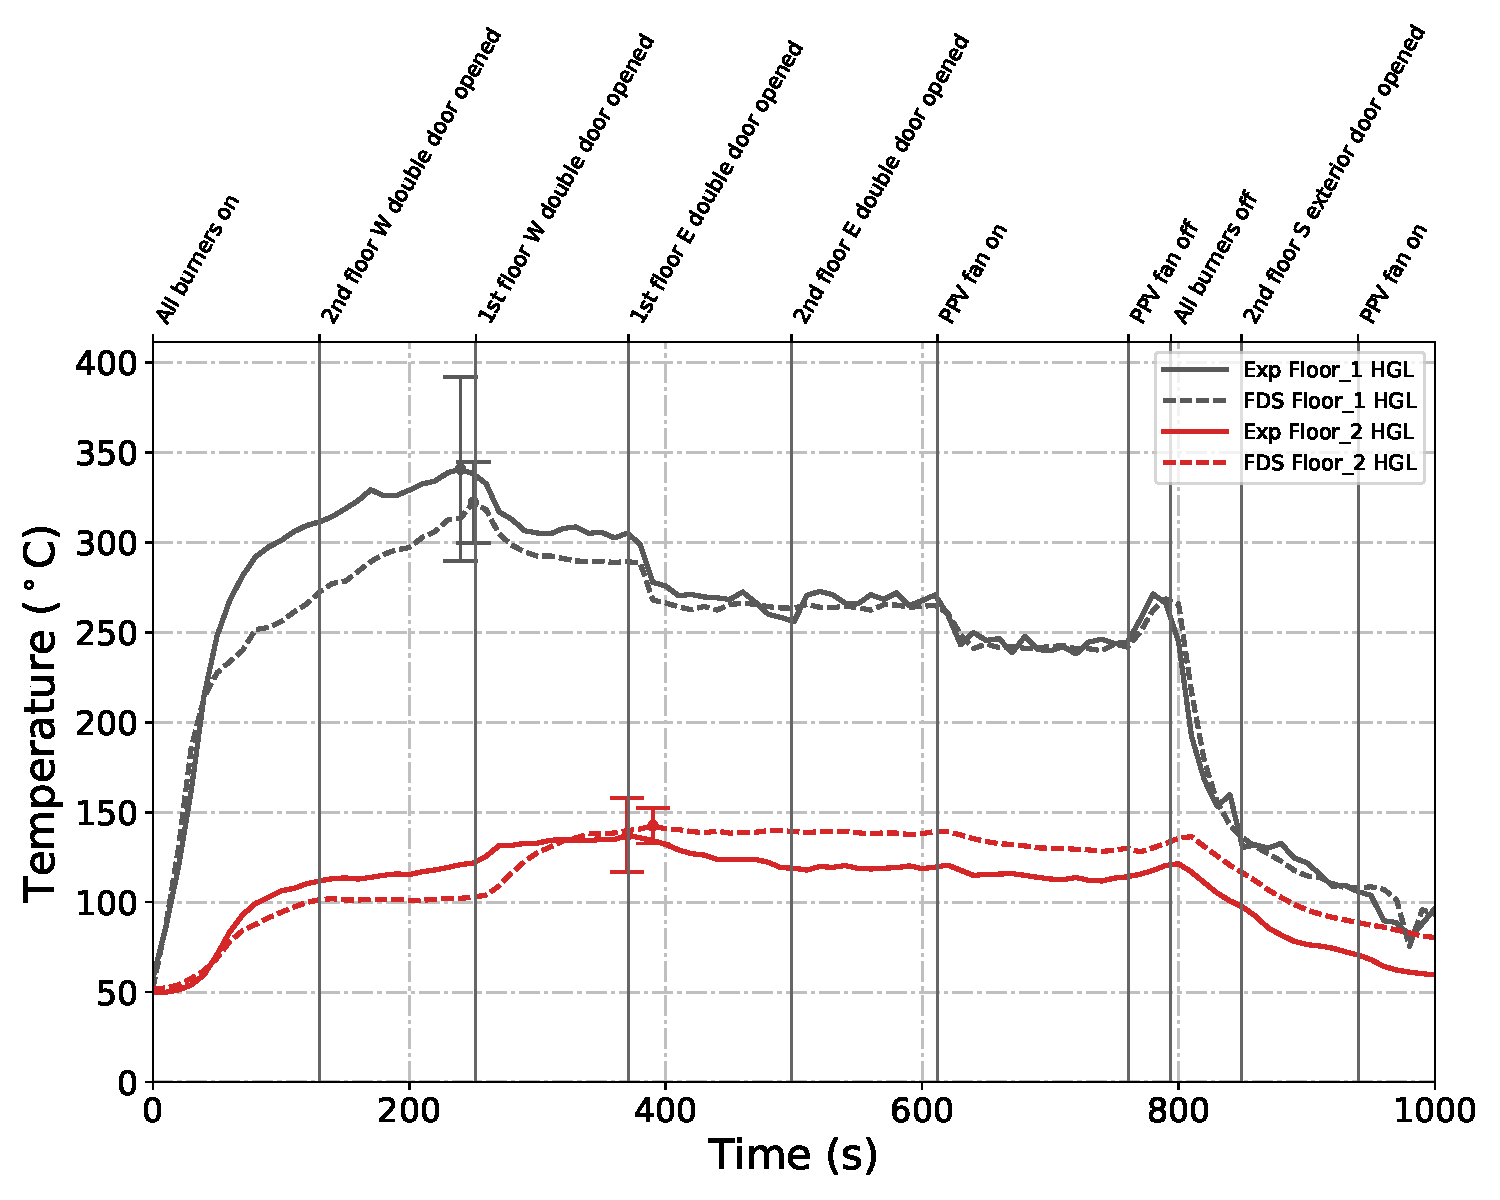
\includegraphics[width=\columnwidth]{Figures/Plots/Validation/Temperature/Test_23_HGL}
	\caption[Plots of measured and predicted hot gas layer temperatures during Test~23.]{Plots of measured and predicted hot gas layer temperatures on the first and second floors of the West Structure during Test~23.}
	\label{fig:HGL_data_Test23}
\end{figure}

\begin{figure}[!h]
	\centering
	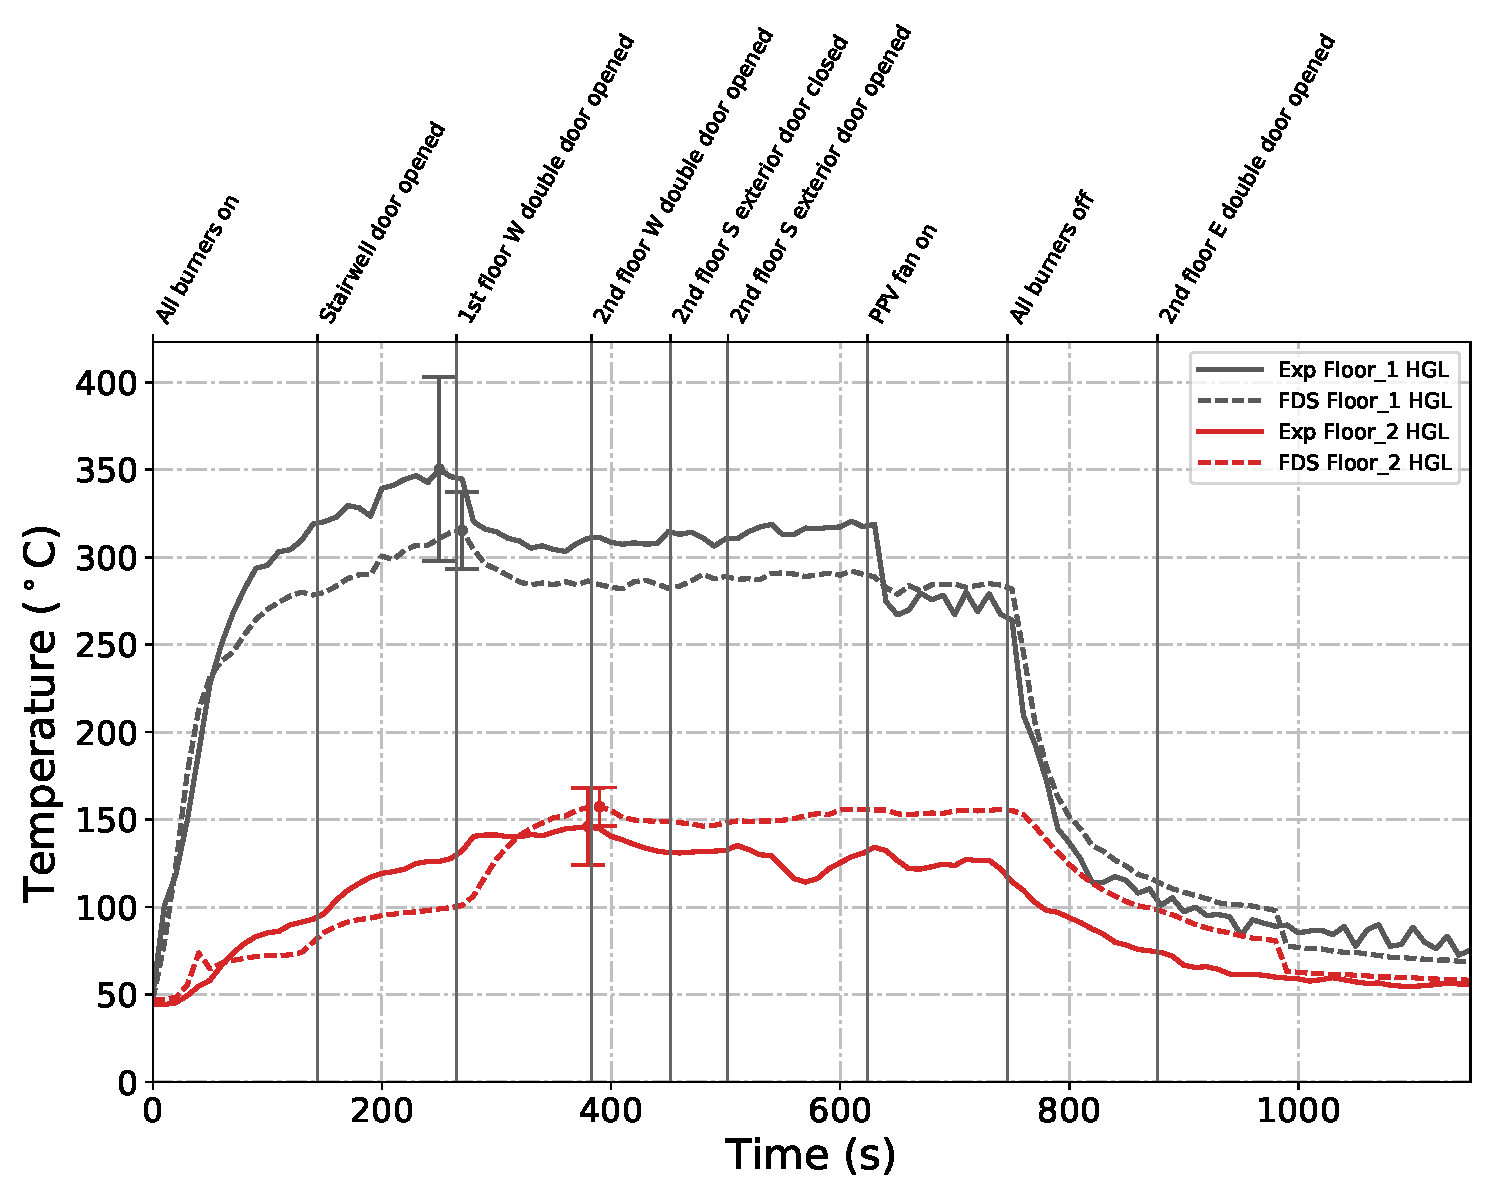
\includegraphics[width=\columnwidth]{Figures/Plots/Validation/Temperature/Test_24_HGL}
	\caption[Plots of measured and predicted hot gas layer temperatures during Test~24.]{Plots of measured and predicted hot gas layer temperatures on the first and second floors of the West Structure during Test~24.}
	\label{fig:HGL_data_Test24}
\end{figure}

\begin{figure}[!h]
	\centering
	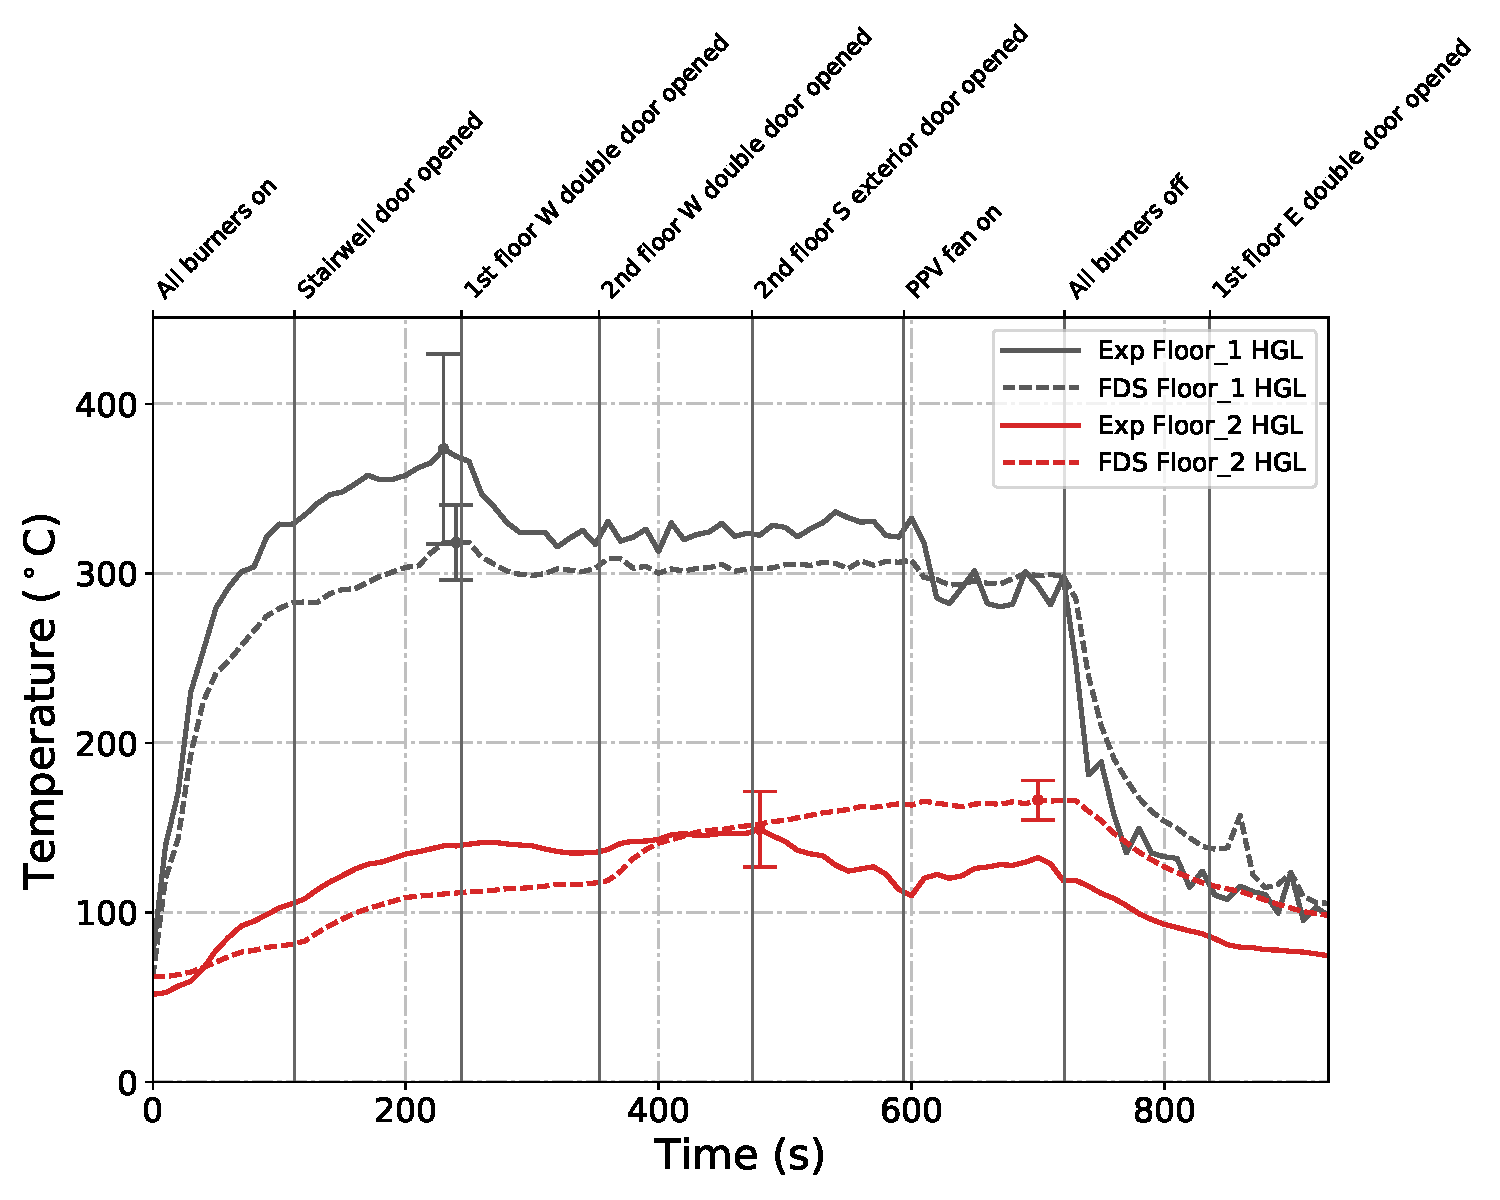
\includegraphics[width=\columnwidth]{Figures/Plots/Validation/Temperature/Test_25_HGL}
	\caption[Plots of measured and predicted hot gas layer temperatures during Test~25.]{Plots of measured and predicted hot gas layer temperatures on the first and second floors of the West Structure during Test~25.}
	\label{fig:HGL_data_Test25}
\end{figure}

\clearpage
\subsection*{\textit{Ceiling Jet Temperatures}}
\begin{figure}[!h]
	\centering
	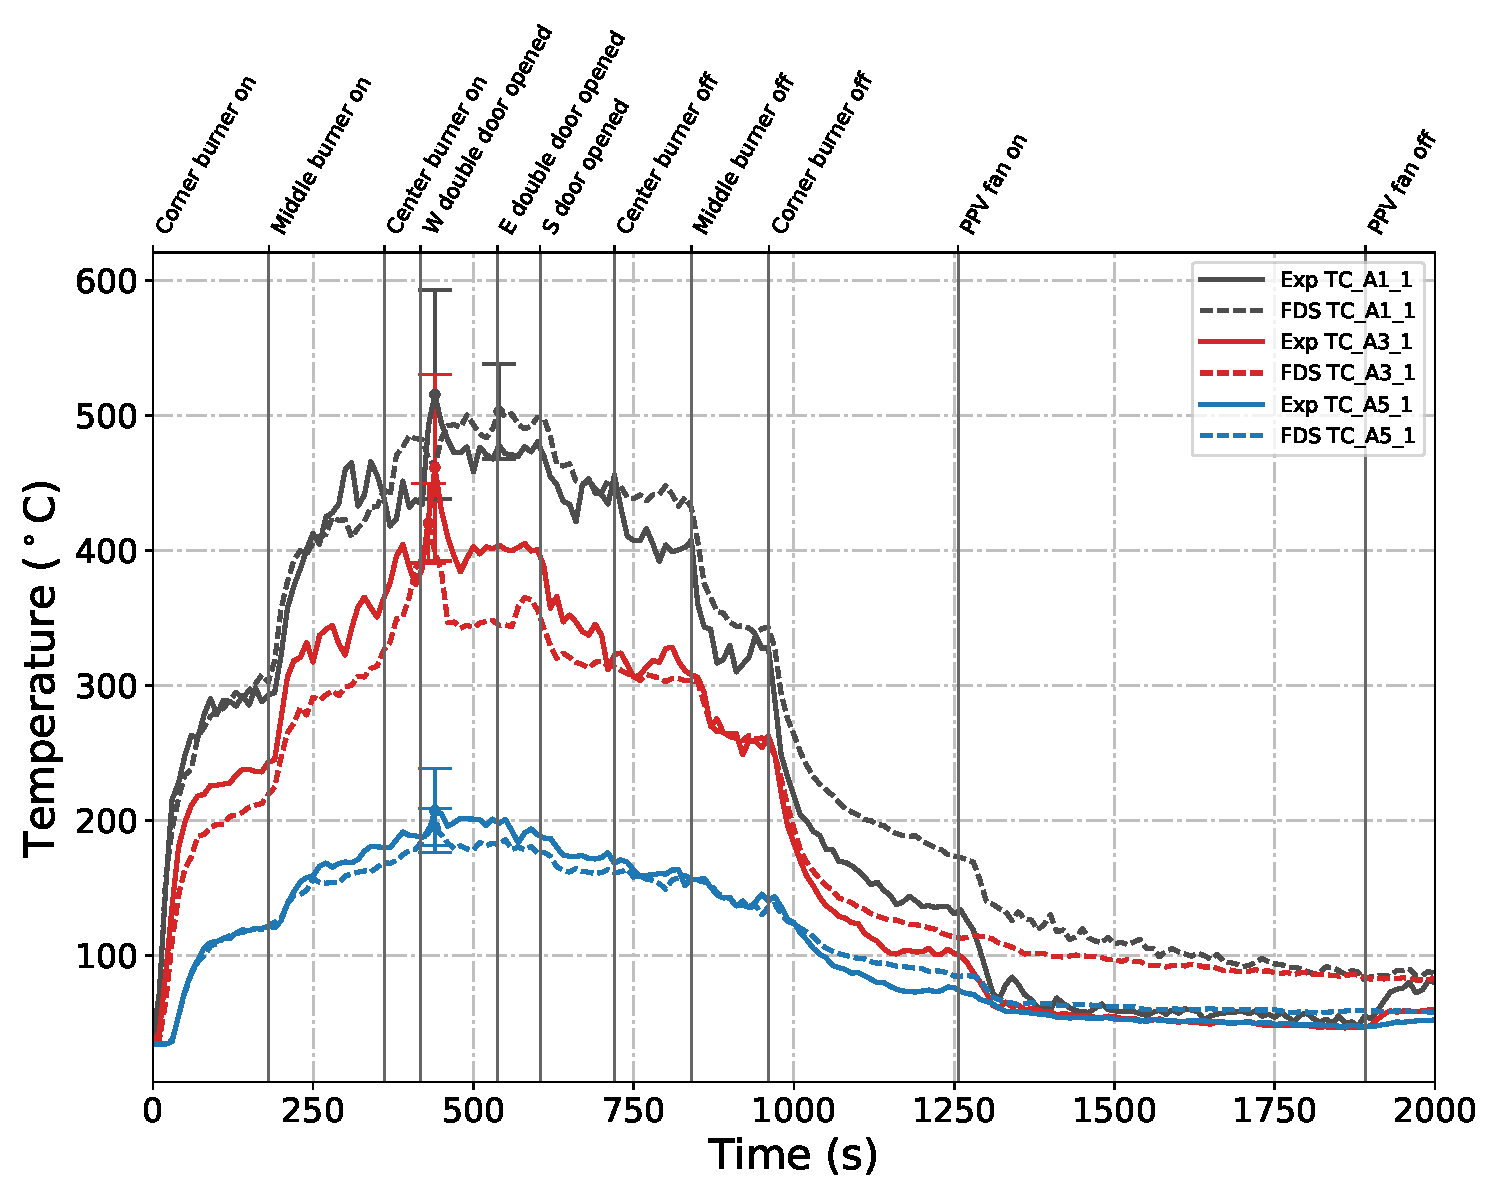
\includegraphics[width=\columnwidth]{Figures/Plots/Validation/Temperature/Test_2_cjet_1}
	\caption[Plots of measured and predicted ceiling jet temperatures during Test~2.]{Plots of measured and predicted ceiling jet temperatures during Test~2 obtained from thermocouple arrays A1, A3, and A5 located in the fire room, middle room, and north room of the East Structure, respectively.}
	\label{fig:cjet1_data_Test2}
\end{figure}

\begin{figure}[!h]
	\centering
	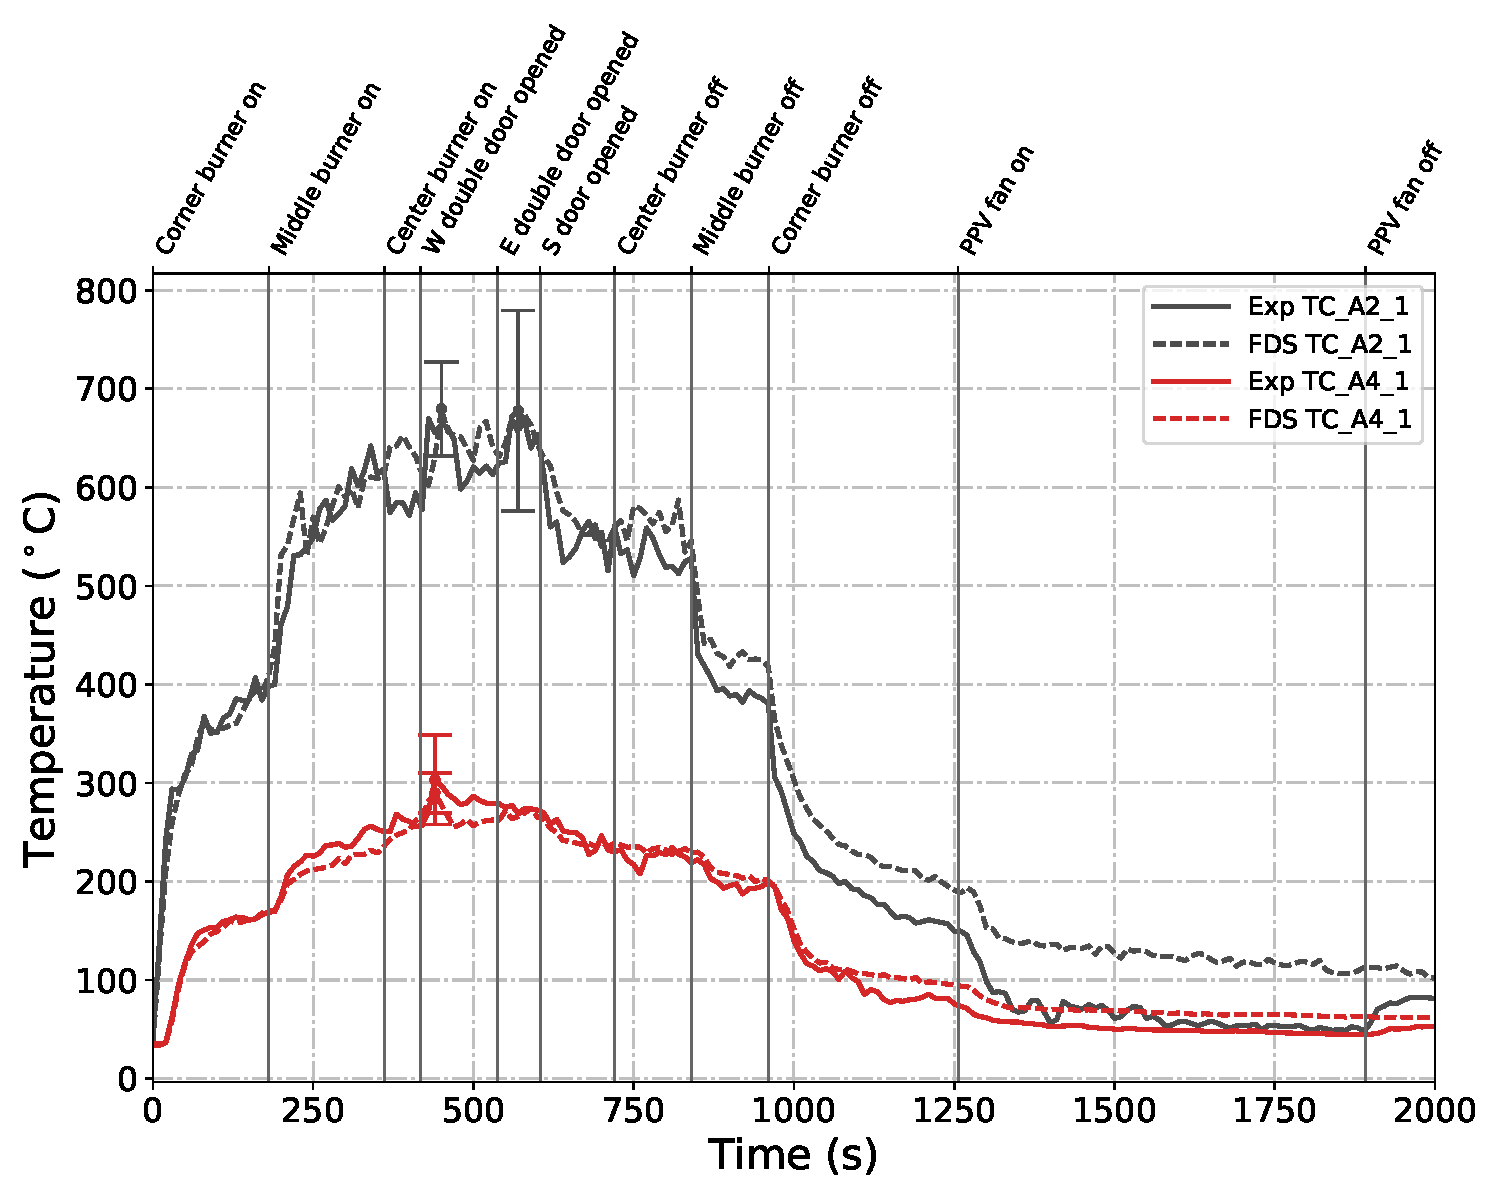
\includegraphics[width=\columnwidth]{Figures/Plots/Validation/Temperature/Test_2_cjet_2}
	\caption[Plots of measured and predicted ceiling jet temperatures during Test~2.]{Plots of measured and predicted ceiling jet temperatures during Test~2 obtained from thermocouple arrays A2 and A4 located in the fire room and north room of the East Structure, respectively.}
	\label{fig:cjet2_data_Test2}
\end{figure}

\begin{figure}[!h]
	\centering
	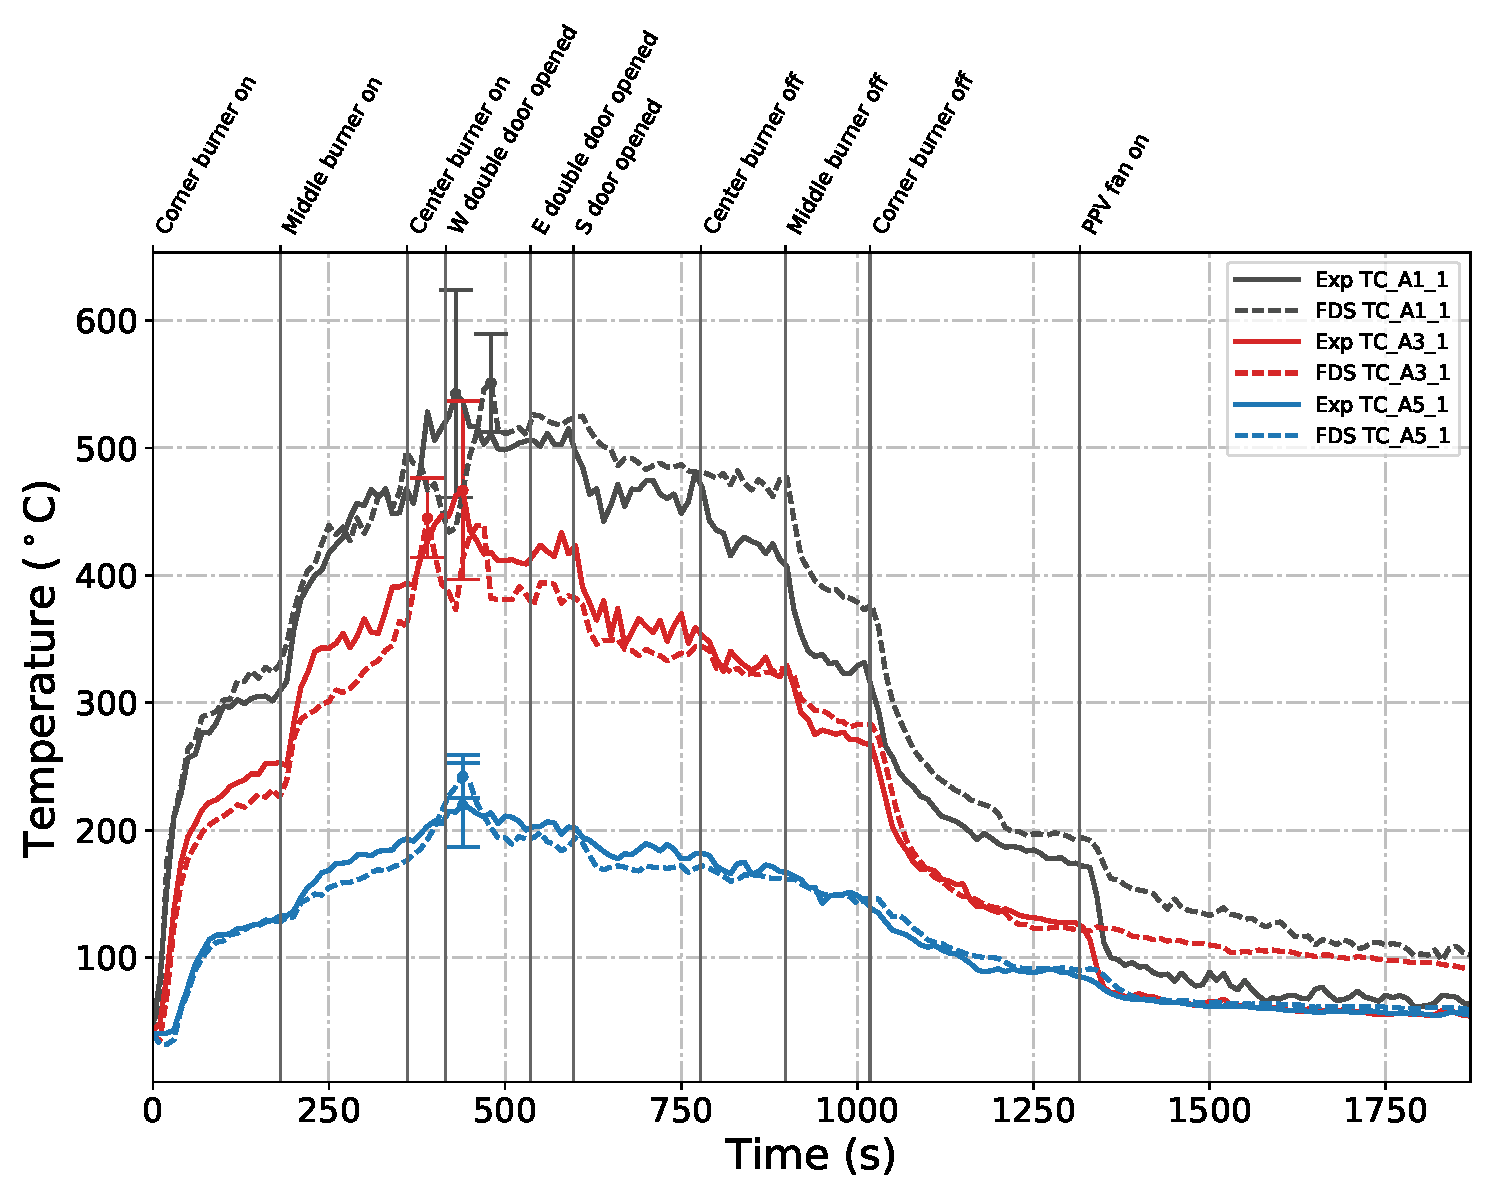
\includegraphics[width=\columnwidth]{Figures/Plots/Validation/Temperature/Test_3_cjet_1}
	\caption[Plots of measured and predicted ceiling jet temperatures during Test~3.]{Plots of measured and predicted ceiling jet temperatures during Test~3 obtained from thermocouple arrays A1, A3, and A5 located in the fire room, middle room, and north room of the East Structure, respectively.}
	\label{fig:cjet1_data_Test3}
\end{figure}

\begin{figure}[!h]
	\centering
	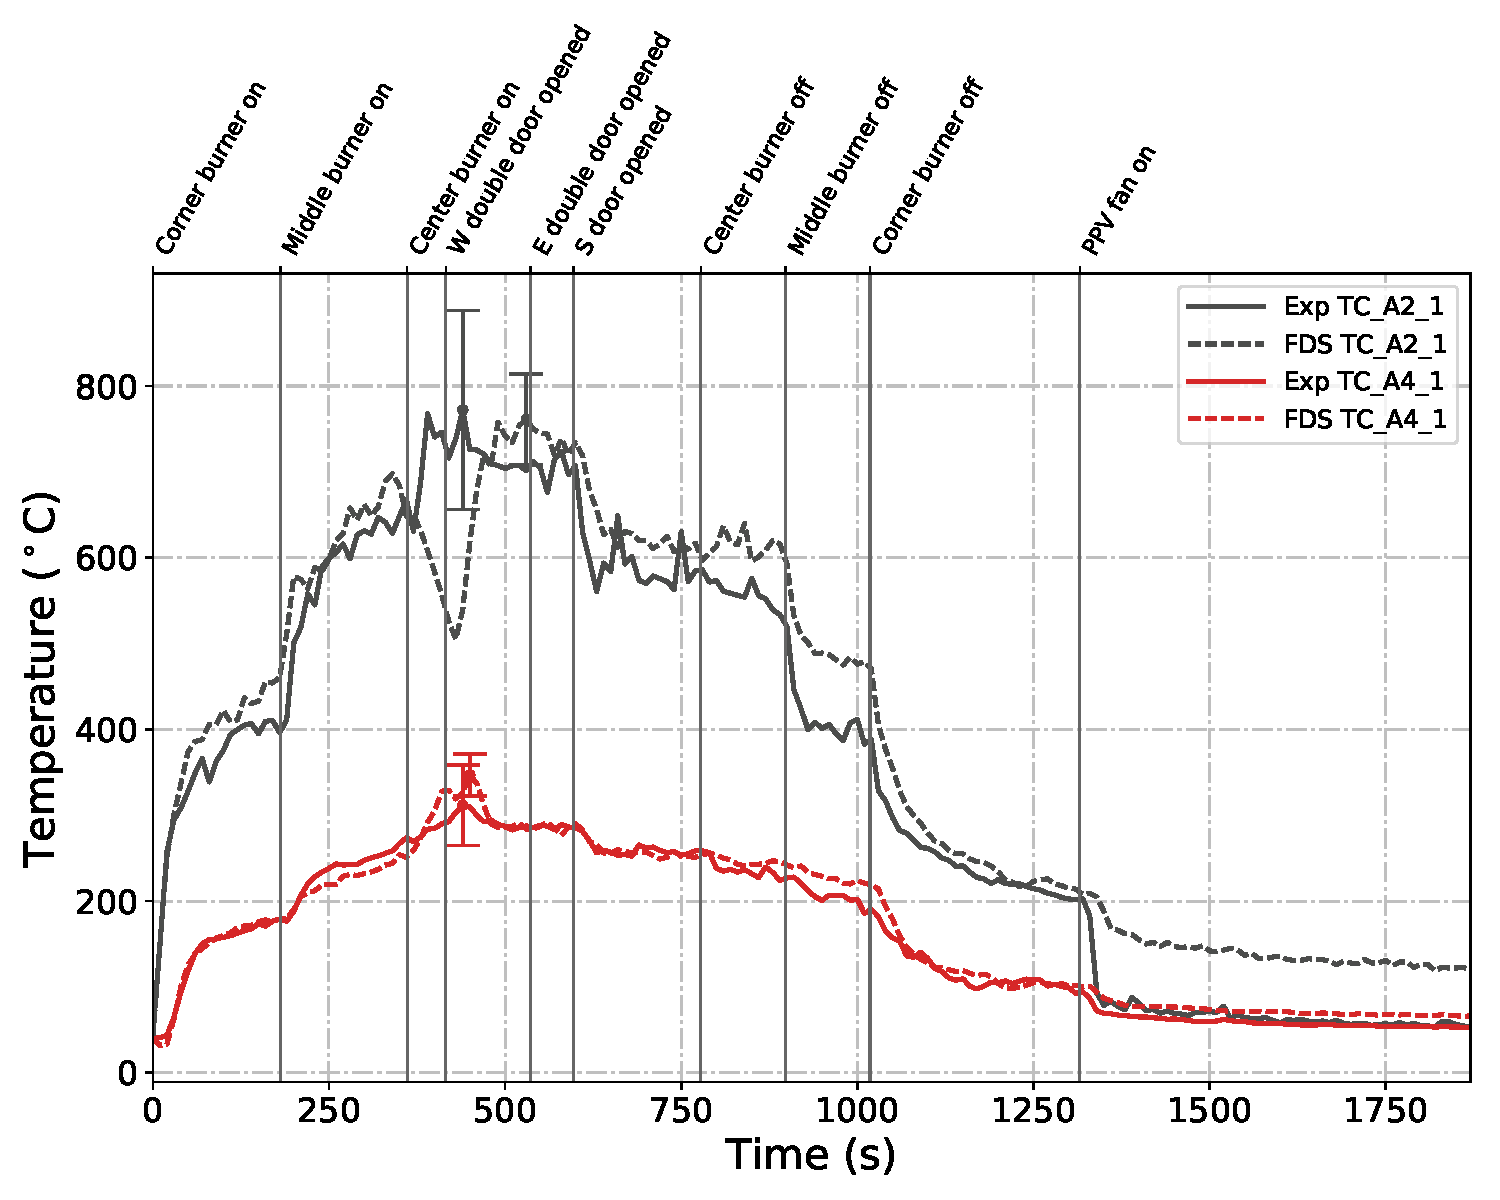
\includegraphics[width=\columnwidth]{Figures/Plots/Validation/Temperature/Test_3_cjet_2}
	\caption[Plots of measured and predicted ceiling jet temperatures during Test~3.]{Plots of measured and predicted ceiling jet temperatures during Test~3 obtained from thermocouple arrays A2 and A4 located in the fire room and north room of the East Structure, respectively.}
	\label{fig:cjet2_data_Test3}
\end{figure}

\begin{figure}[!h]
	\centering
	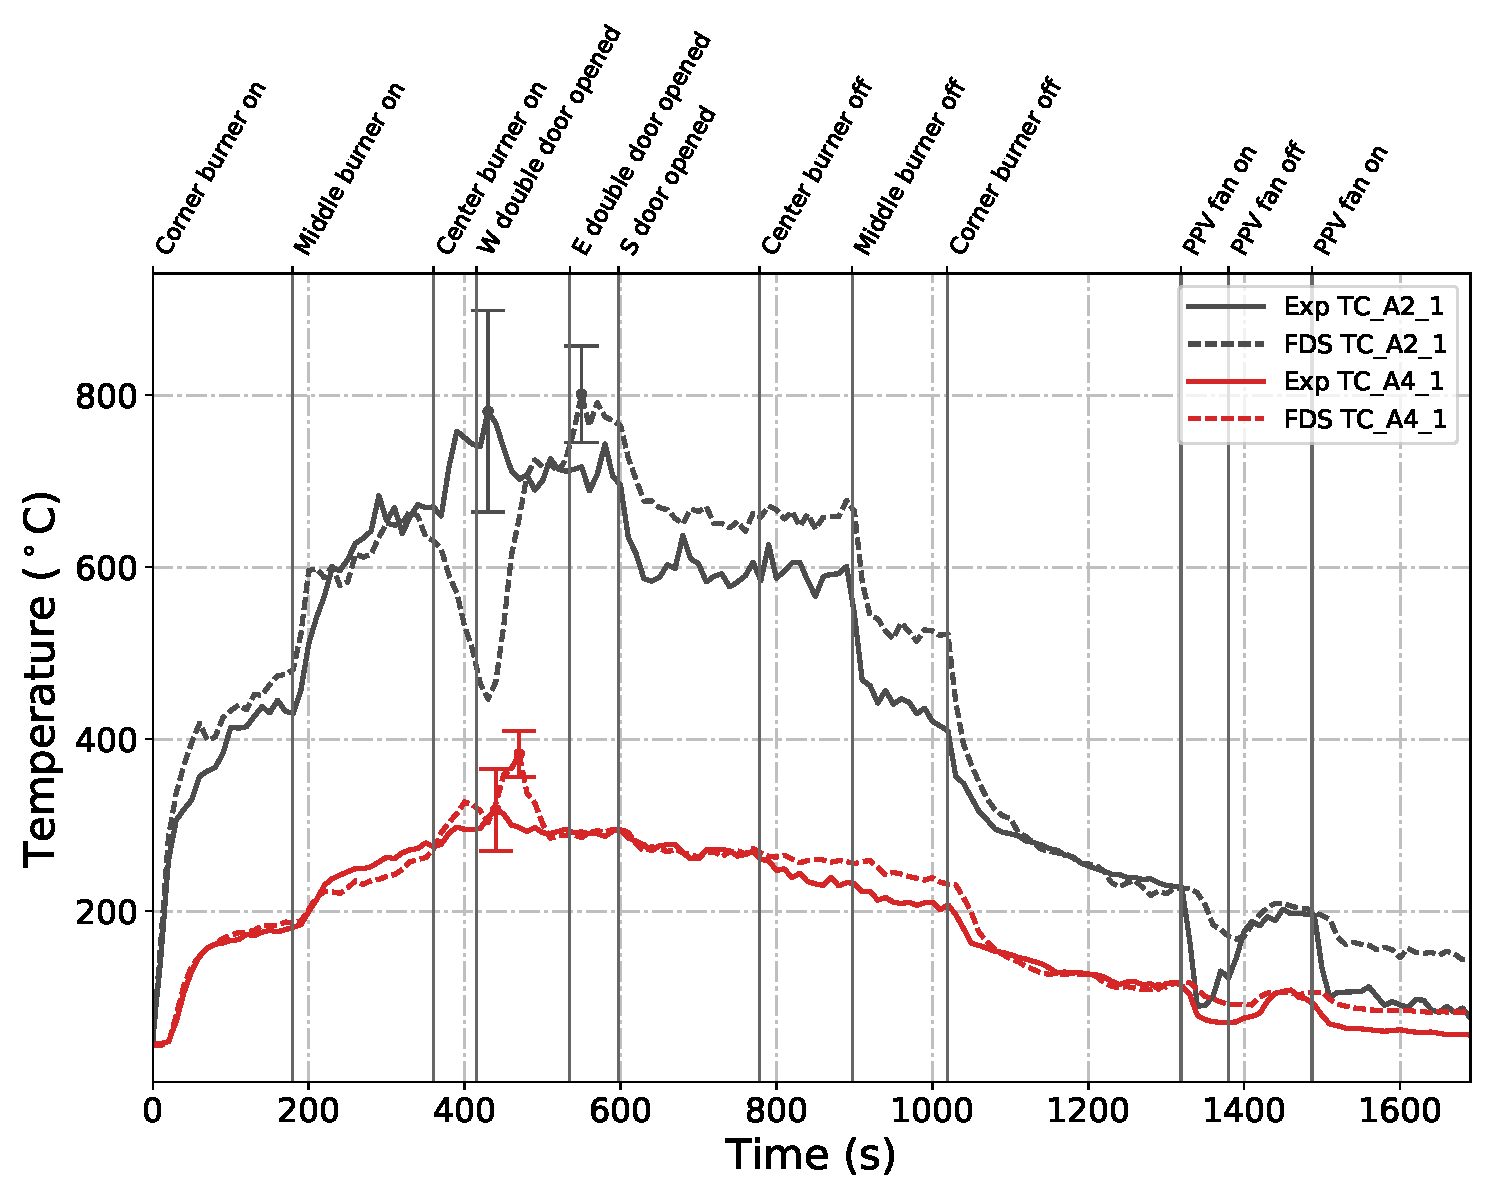
\includegraphics[width=\columnwidth]{Figures/Plots/Validation/Temperature/Test_4_cjet_2}
	\caption[Plots of measured and predicted ceiling jet temperatures during Test~4.]{Plots of measured and predicted ceiling jet temperatures during Test~4 obtained from thermocouple arrays A2 and A4 located in the fire room and north room of the East Structure, respectively.}
	\label{fig:cjet2_data_Test4}
\end{figure}

\begin{figure}[!h]
	\centering
	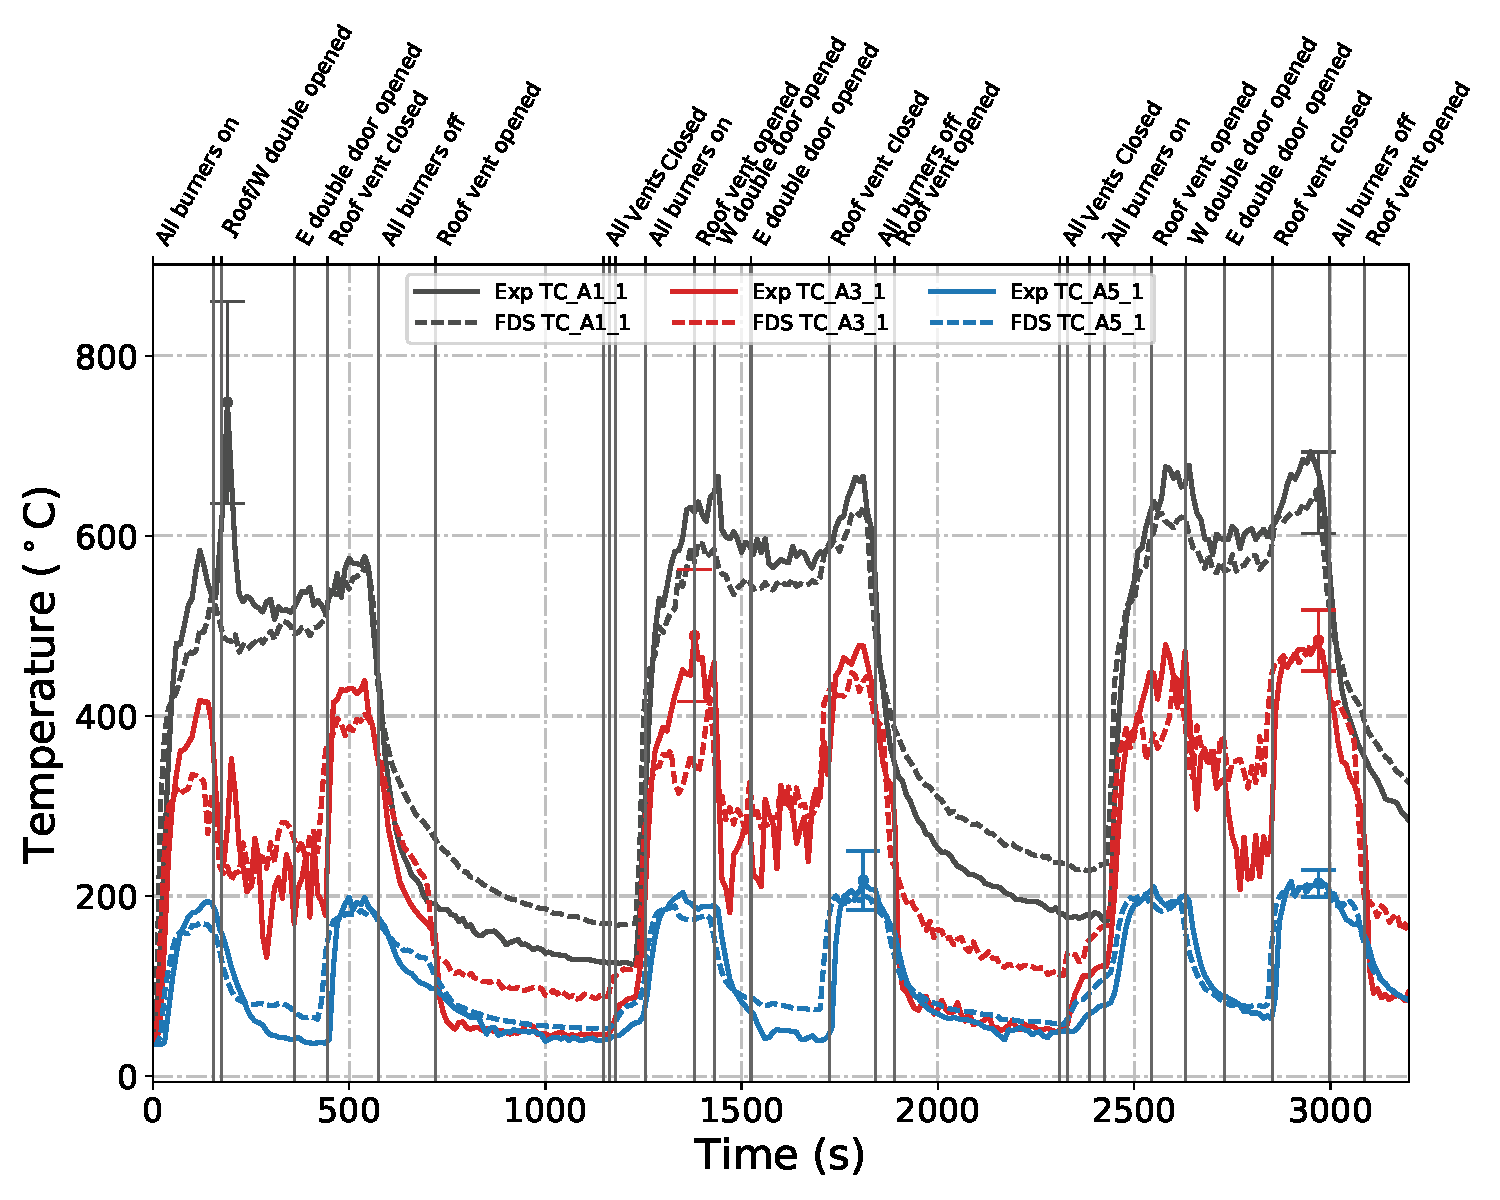
\includegraphics[width=\columnwidth]{Figures/Plots/Validation/Temperature/Test_5_cjet_1}
	\caption[Plots of measured and predicted ceiling jet temperatures during Test~5.]{Plots of measured and predicted ceiling jet temperatures during Test~5 obtained from thermocouple arrays A1, A3, and A5 located in the fire room, middle room, and north room of the East Structure, respectively.}
	\label{fig:cjet1_data_Test5}
\end{figure}

\begin{figure}[!h]
	\centering
	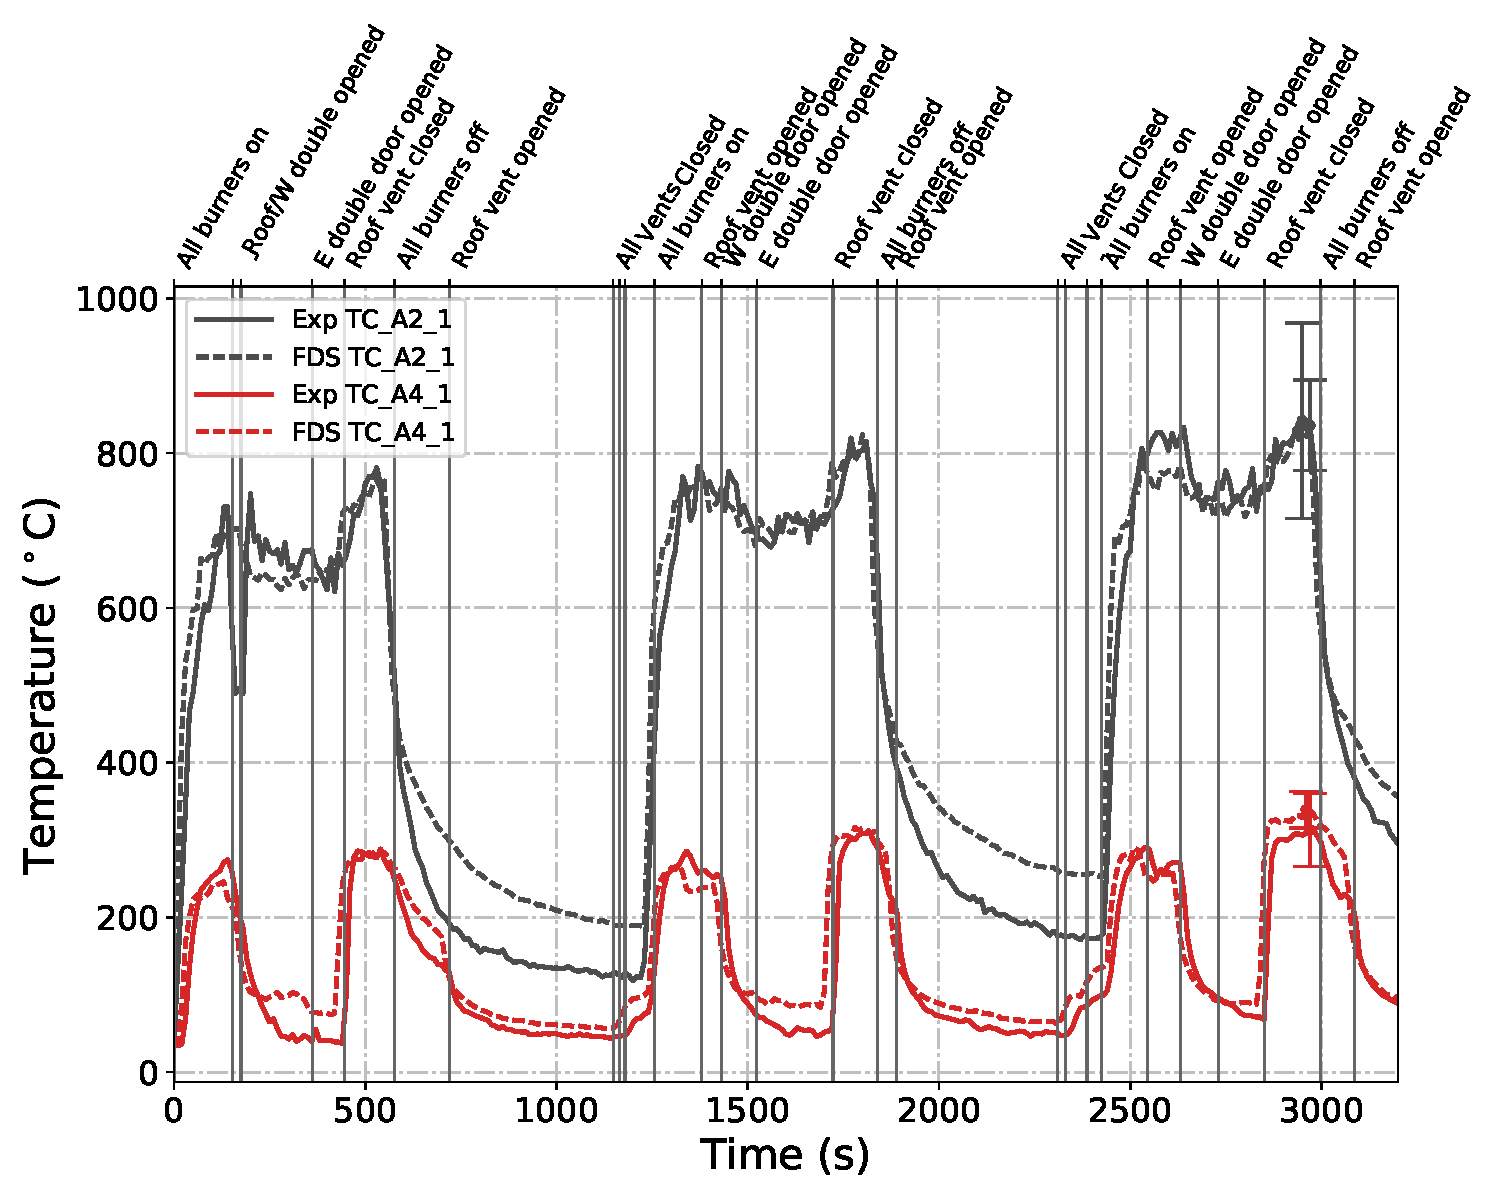
\includegraphics[width=\columnwidth]{Figures/Plots/Validation/Temperature/Test_5_cjet_2}
	\caption[Plots of measured and predicted ceiling jet temperatures during Test~5.]{Plots of measured and predicted ceiling jet temperatures during Test~5 obtained from thermocouple arrays A2 and A4 located in the fire room and north room of the East Structure, respectively.}
	\label{fig:cjet2_data_Test5}
\end{figure}

\begin{figure}[!h]
	\centering
	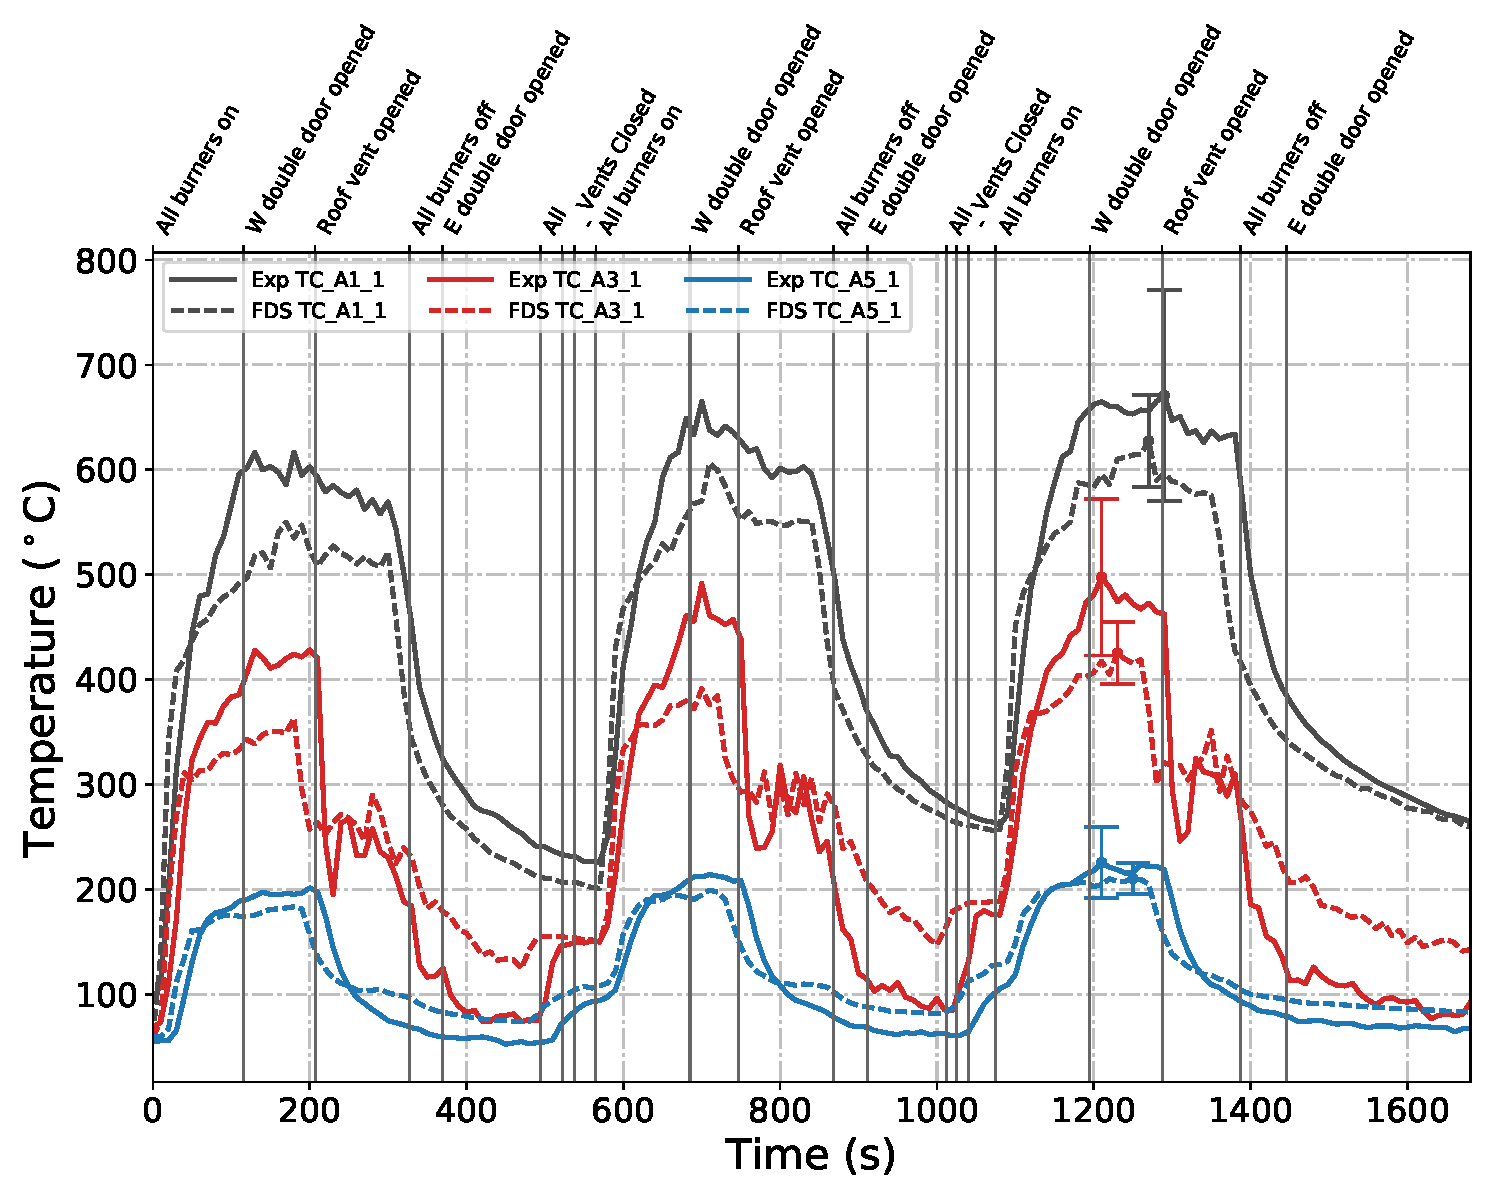
\includegraphics[width=\columnwidth]{Figures/Plots/Validation/Temperature/Test_6_cjet_1}
	\caption[Plots of measured and predicted ceiling jet temperatures during Test~6.]{Plots of measured and predicted ceiling jet temperatures during Test~6 obtained from thermocouple arrays A1, A3, and A5 located in the fire room, middle room, and north room of the East Structure, respectively.}
	\label{fig:cjet1_data_Test6}
\end{figure}

\begin{figure}[!h]
	\centering
	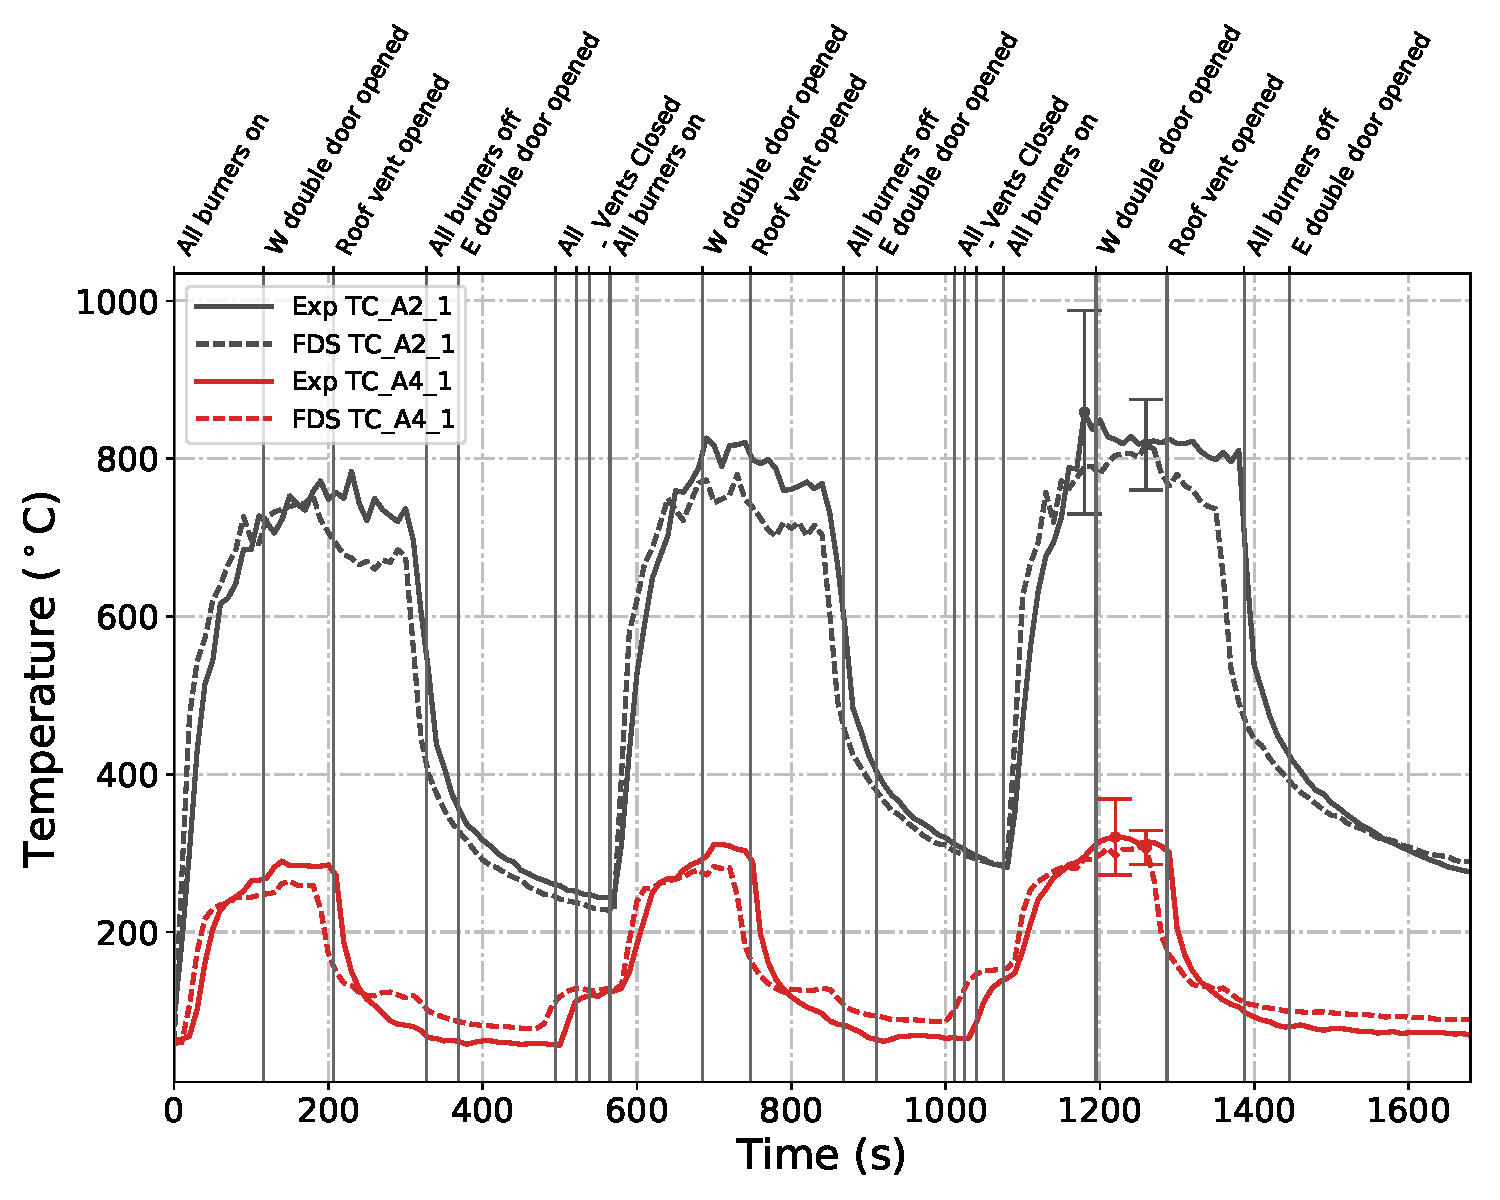
\includegraphics[width=\columnwidth]{Figures/Plots/Validation/Temperature/Test_6_cjet_2}
	\caption[Plots of measured and predicted ceiling jet temperatures during Test~6.]{Plots of measured and predicted ceiling jet temperatures during Test~6 obtained from thermocouple arrays A2 and A4 located in the fire room and north room of the East Structure, respectively.}
	\label{fig:cjet2_data_Test6}
\end{figure}

\begin{figure}[!h]
	\centering
	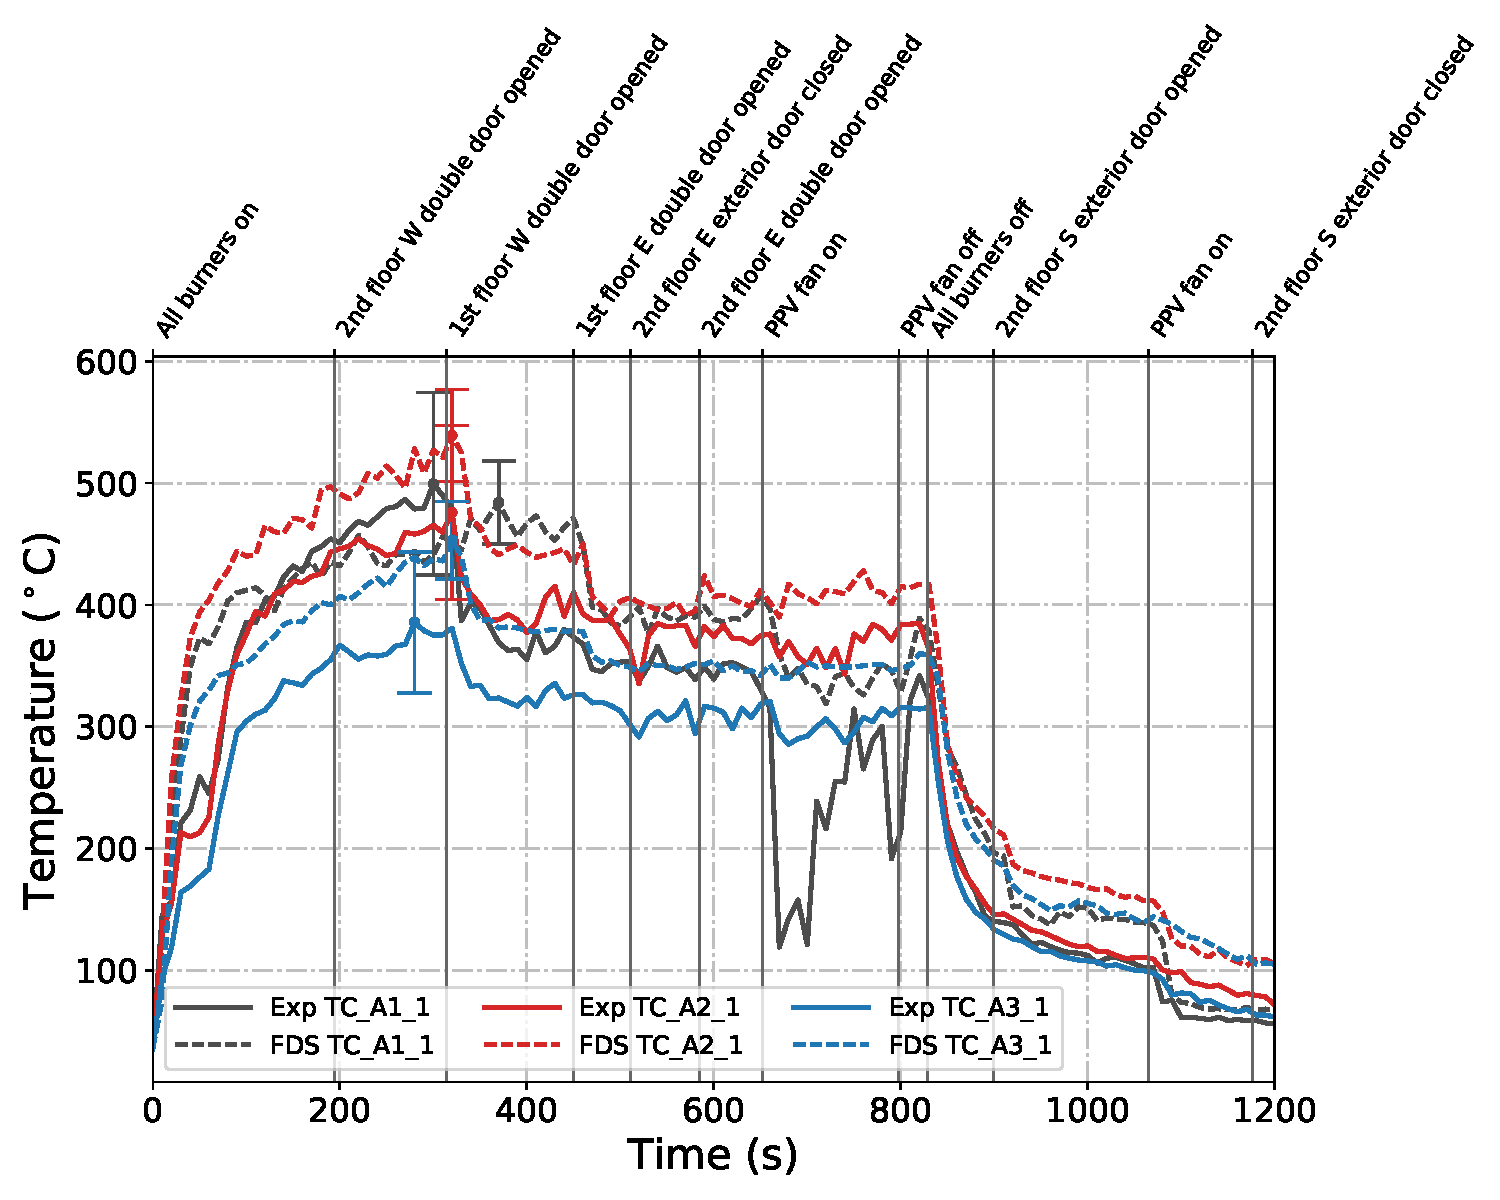
\includegraphics[width=\columnwidth]{Figures/Plots/Validation/Temperature/Test_22_cjet_1}
	\caption[Plots of measured and predicted ceiling jet temperatures on the first floor during Test~22.]{Plots of measured and predicted ceiling jet temperatures on the first floor of the West Structure during Test~22.}
	\label{fig:cjet1_data_Test22}
\end{figure}

\begin{figure}[!h]
	\centering
	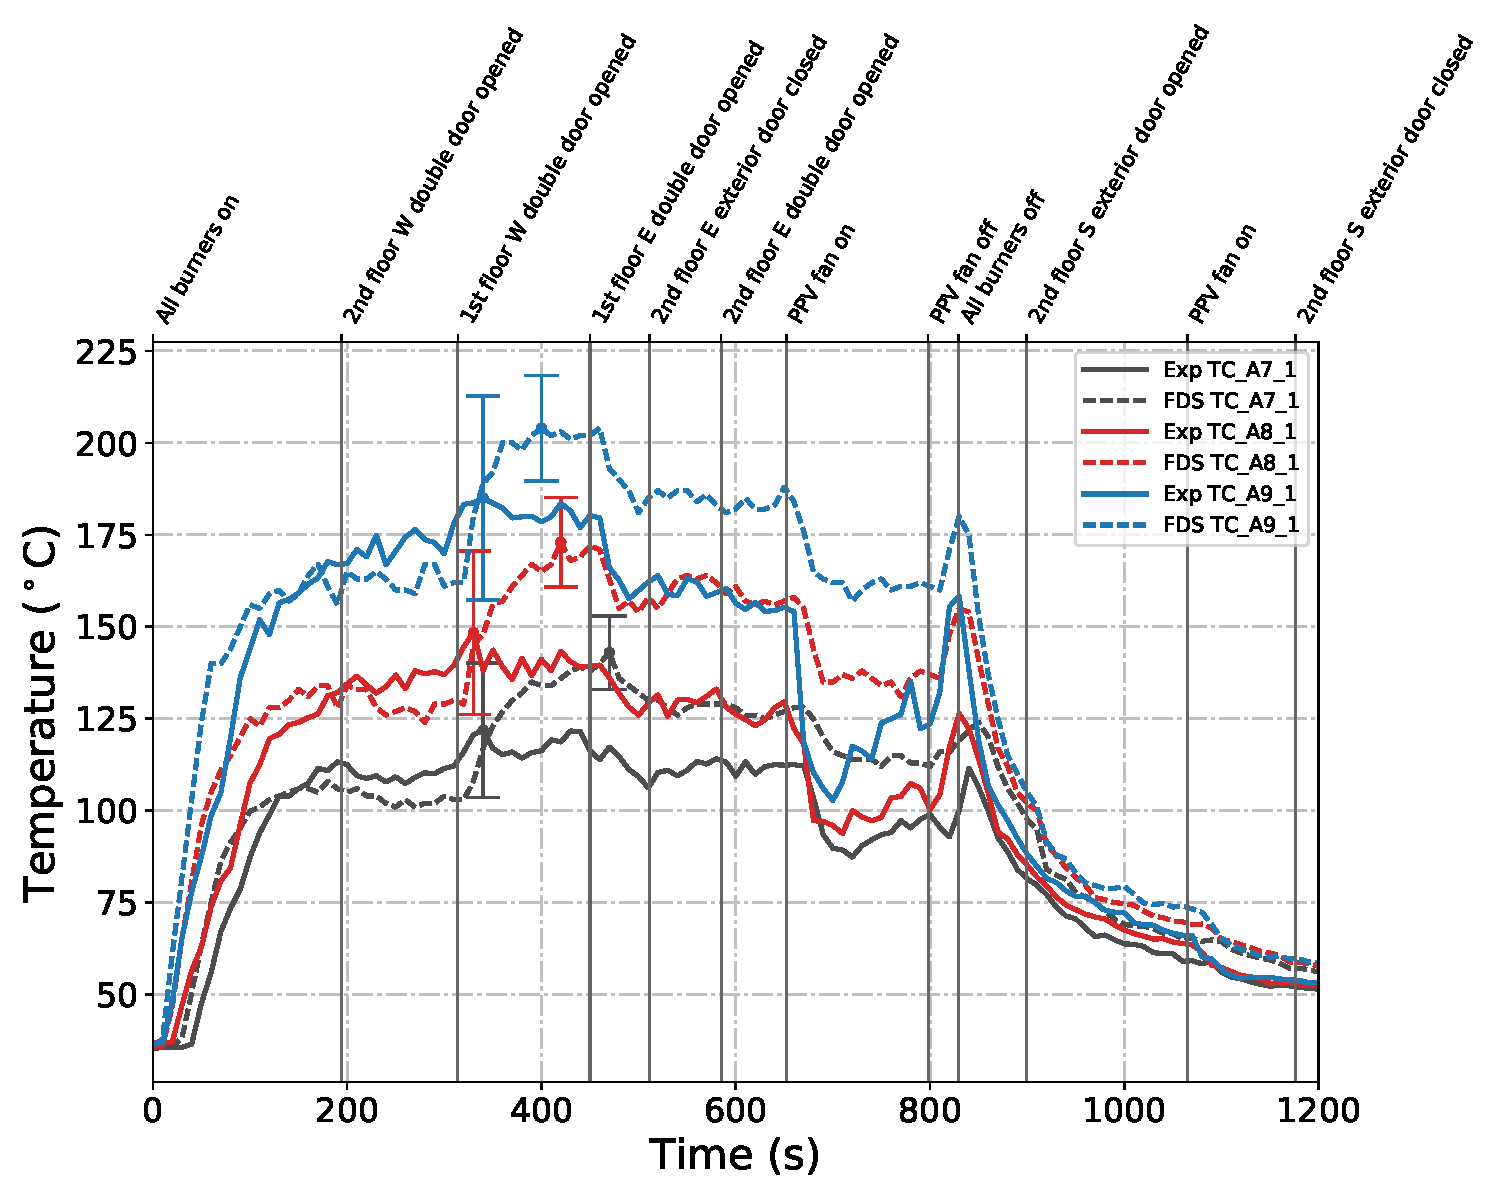
\includegraphics[width=\columnwidth]{Figures/Plots/Validation/Temperature/Test_22_cjet_2}
	\caption[Plots of measured and predicted ceiling jet temperatures on the second floor during Test~22.]{Plots of measured and predicted ceiling jet temperatures on the second floor of the West Structure during Test~22.}
	\label{fig:cjet2_data_Test22}
\end{figure}

\begin{figure}[!h]
	\centering
	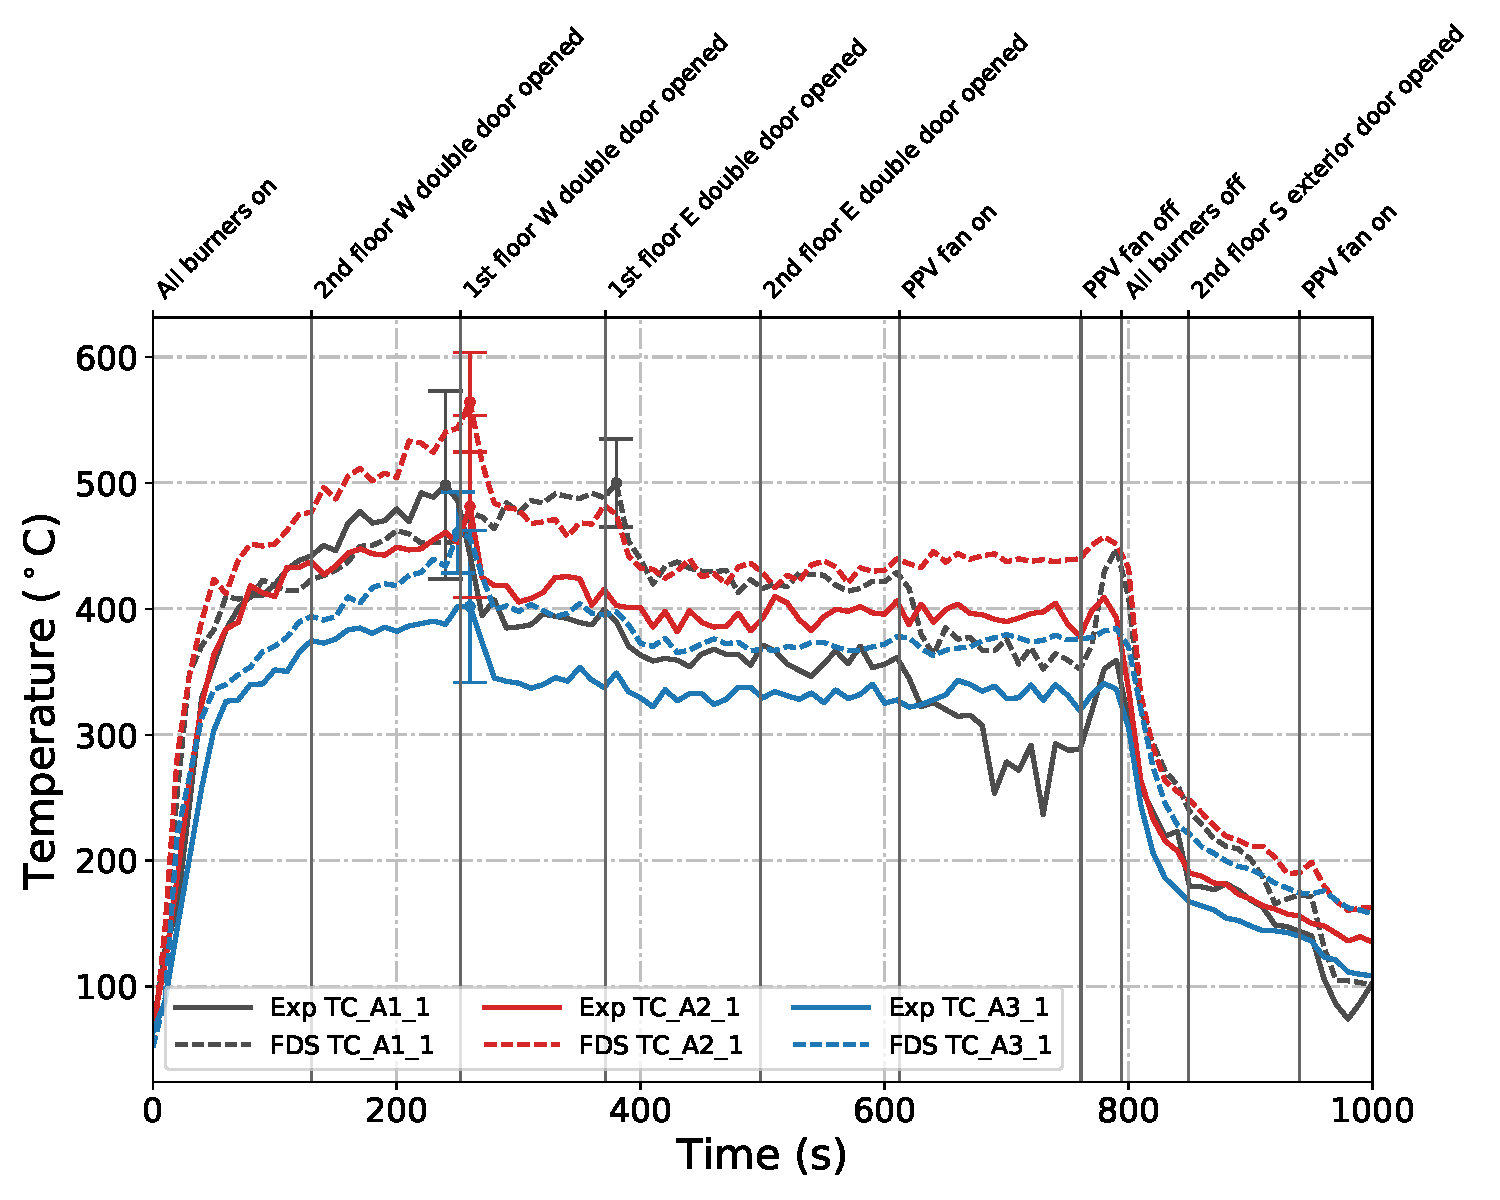
\includegraphics[width=\columnwidth]{Figures/Plots/Validation/Temperature/Test_23_cjet_1}
	\caption[Plots of measured and predicted ceiling jet temperatures on the first floor during Test~23.]{Plots of measured and predicted ceiling jet temperatures on the first floor of the West Structure during Test~23.}
	\label{fig:cjet1_data_Test23}
\end{figure}

\begin{figure}[!h]
	\centering
	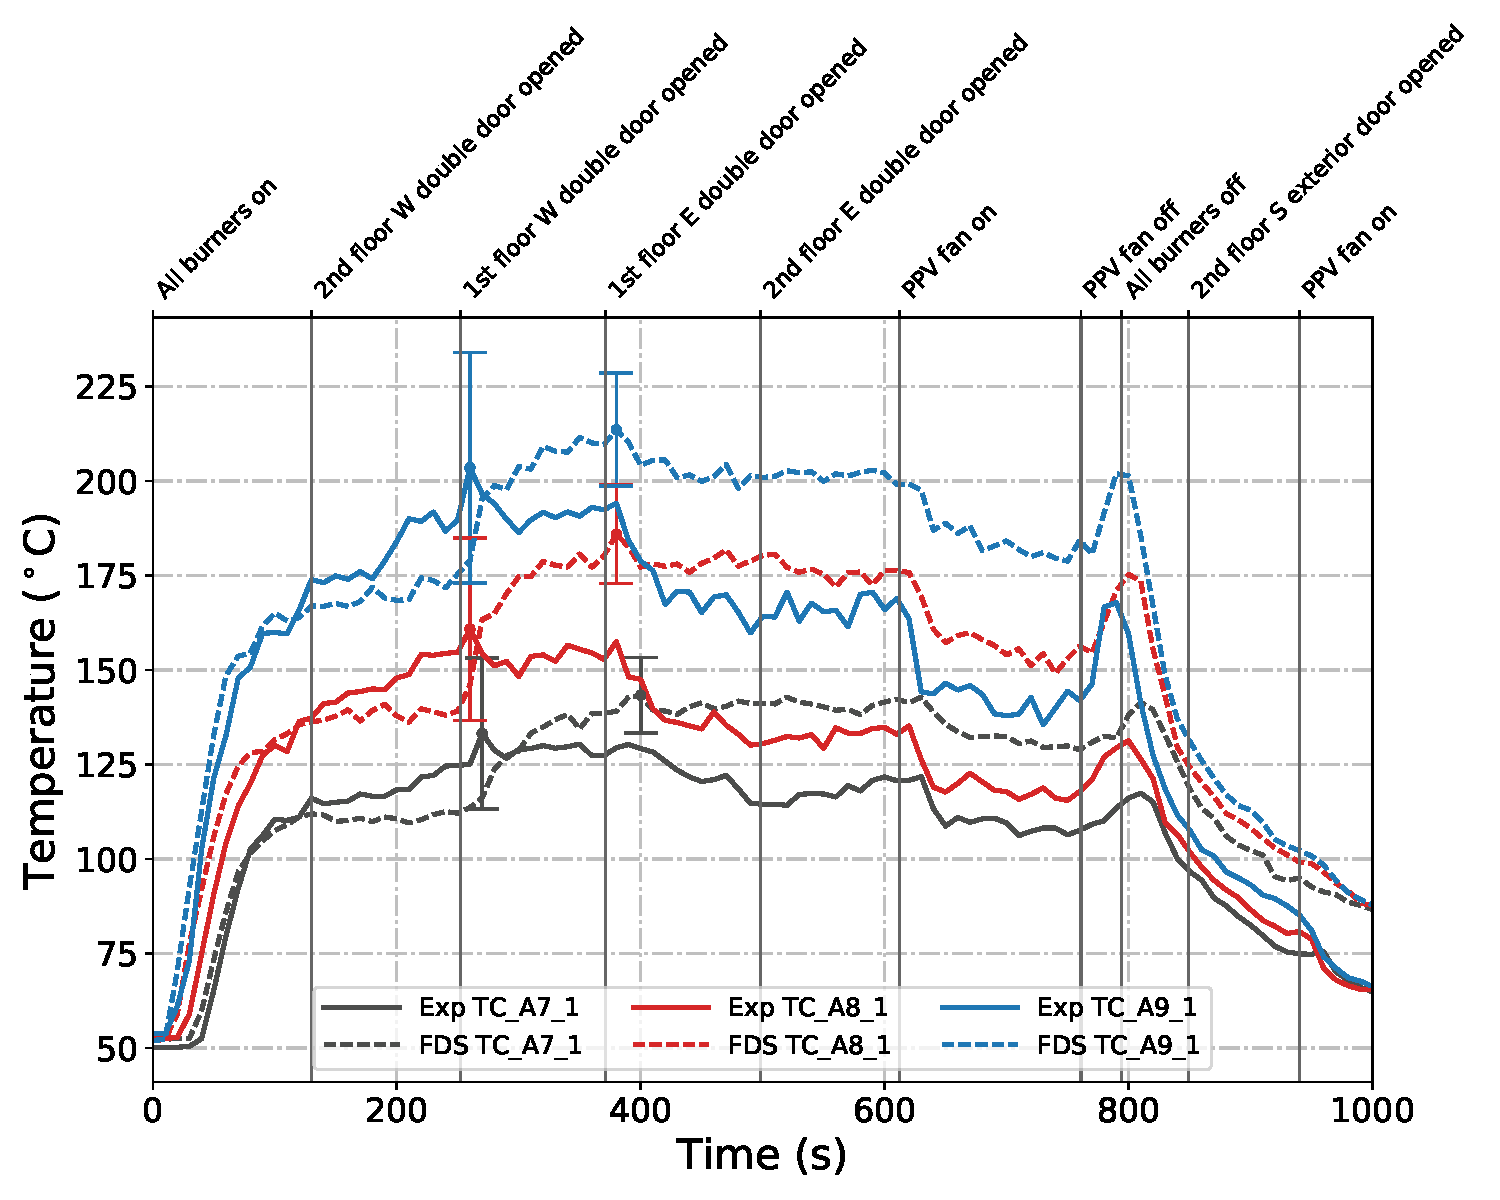
\includegraphics[width=\columnwidth]{Figures/Plots/Validation/Temperature/Test_23_cjet_2}
	\caption[Plots of measured and predicted ceiling jet temperatures on the second floor during Test~23.]{Plots of measured and predicted ceiling jet temperatures on the second floor of the West Structure during Test~23.}
	\label{fig:cjet2_data_Test23}
\end{figure}

\begin{figure}[!h]
	\centering
	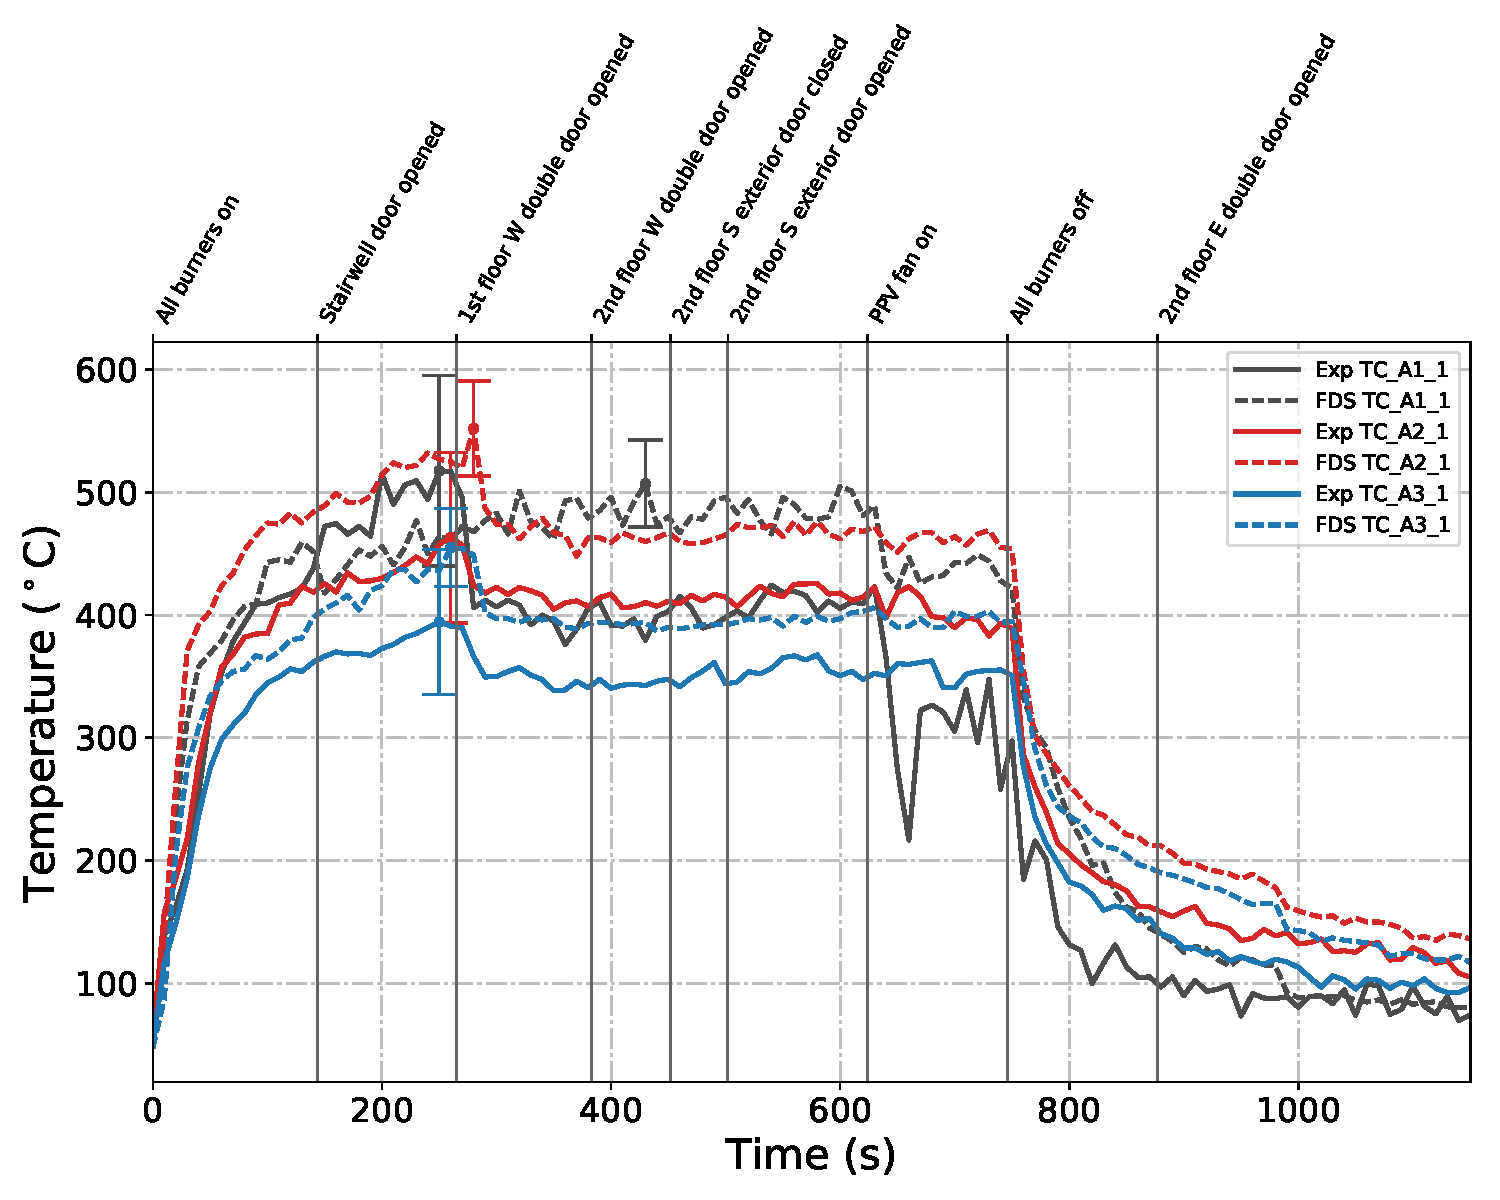
\includegraphics[width=\columnwidth]{Figures/Plots/Validation/Temperature/Test_24_cjet_1}
	\caption[Plots of measured and predicted ceiling jet temperatures on the first floor during Test~24.]{Plots of measured and predicted ceiling jet temperatures on the first floor of the West Structure during Test~24.}
	\label{fig:cjet1_data_Test24}
\end{figure}

\begin{figure}[!h]
	\centering
	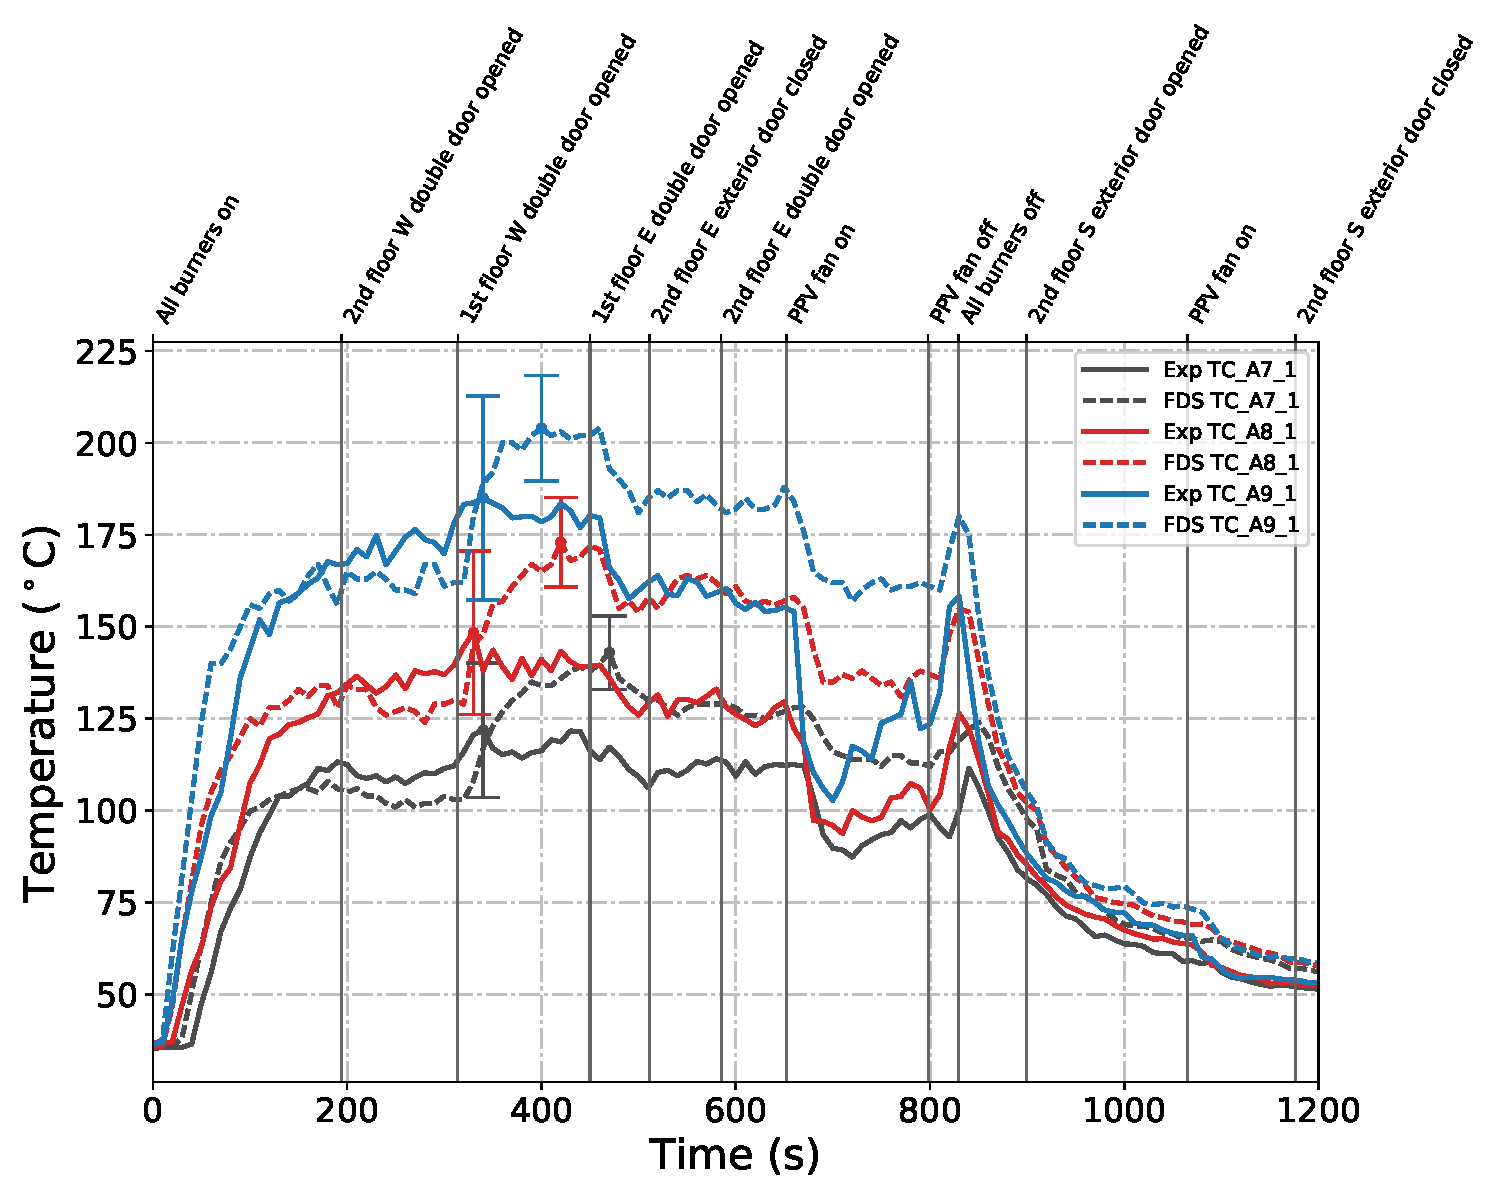
\includegraphics[width=\columnwidth]{Figures/Plots/Validation/Temperature/Test_22_cjet_2}
	\caption[Plots of measured and predicted ceiling jet temperatures on the second floor during Test~24.]{Plots of measured and predicted ceiling jet temperatures on the second floor of the West Structure during Test~24.}
	\label{fig:cjet2_data_Test24}
\end{figure}

\begin{figure}[!h]
	\centering
	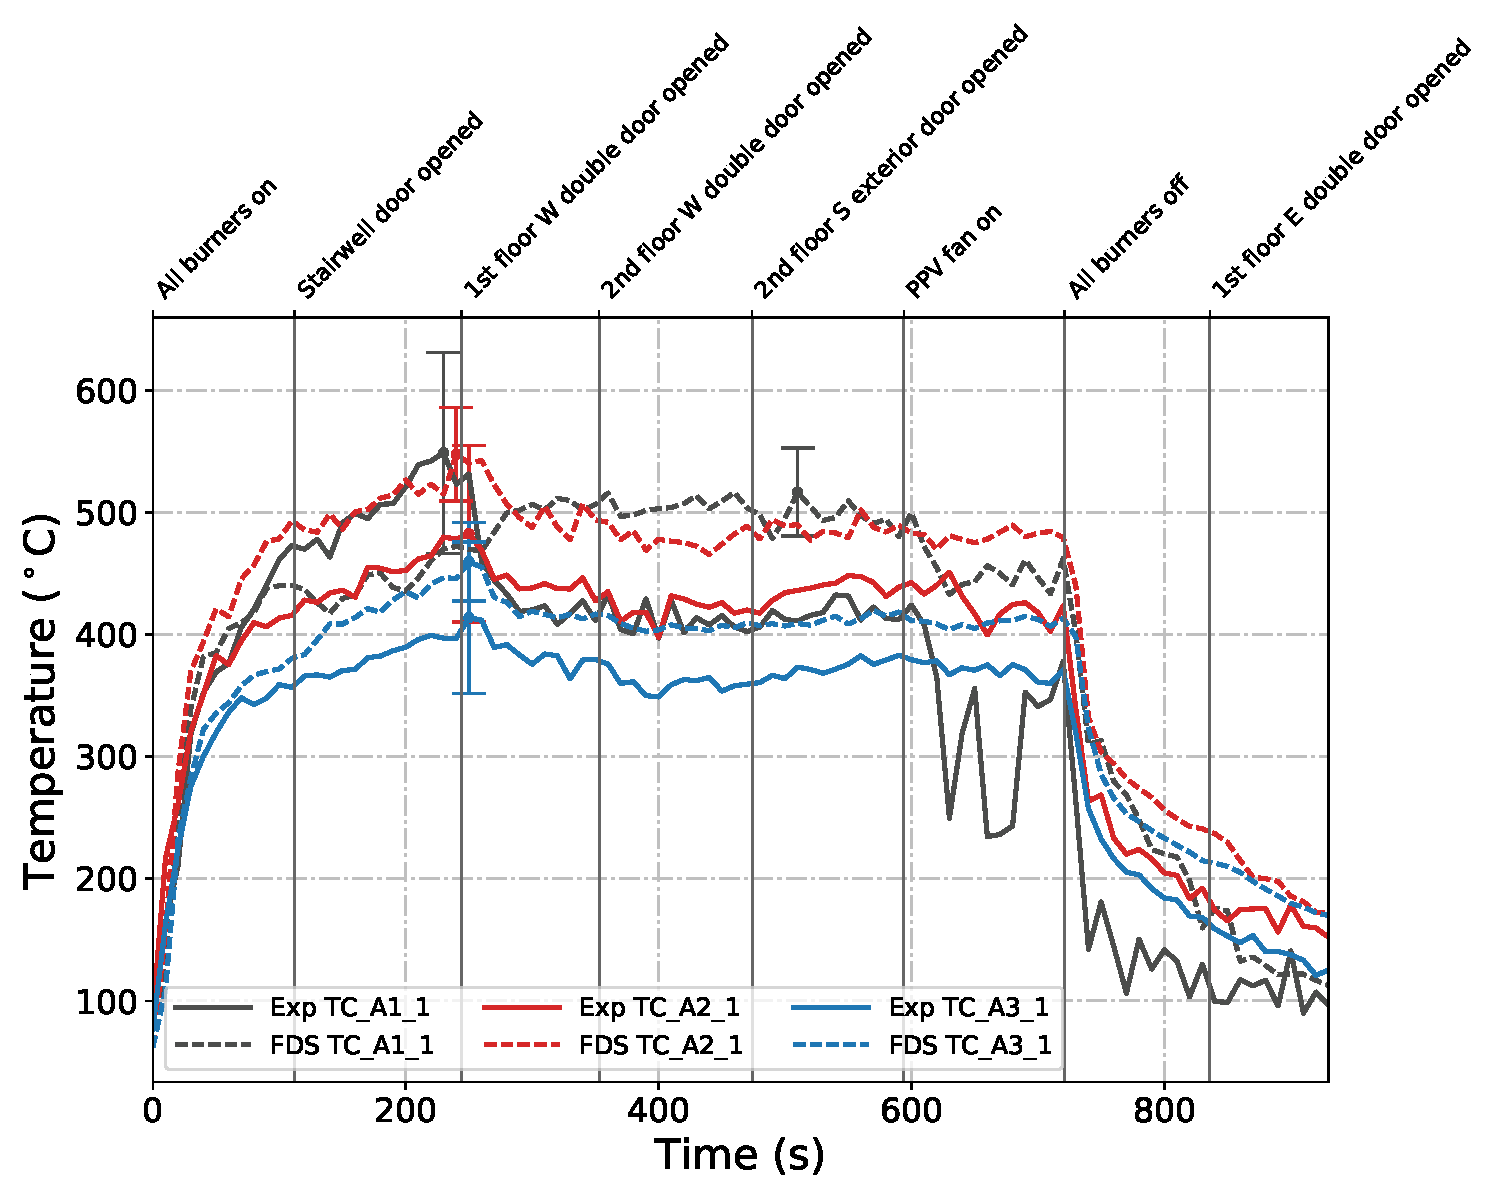
\includegraphics[width=\columnwidth]{Figures/Plots/Validation/Temperature/Test_25_cjet_1}
	\caption[Plots of measured and predicted ceiling jet temperatures on the first floor during Test~25.]{Plots of measured and predicted ceiling jet temperatures on the first floor of the West Structure during Test~25.}
	\label{fig:cjet1_data_Test25}
\end{figure}

\begin{figure}[!h]
	\centering
	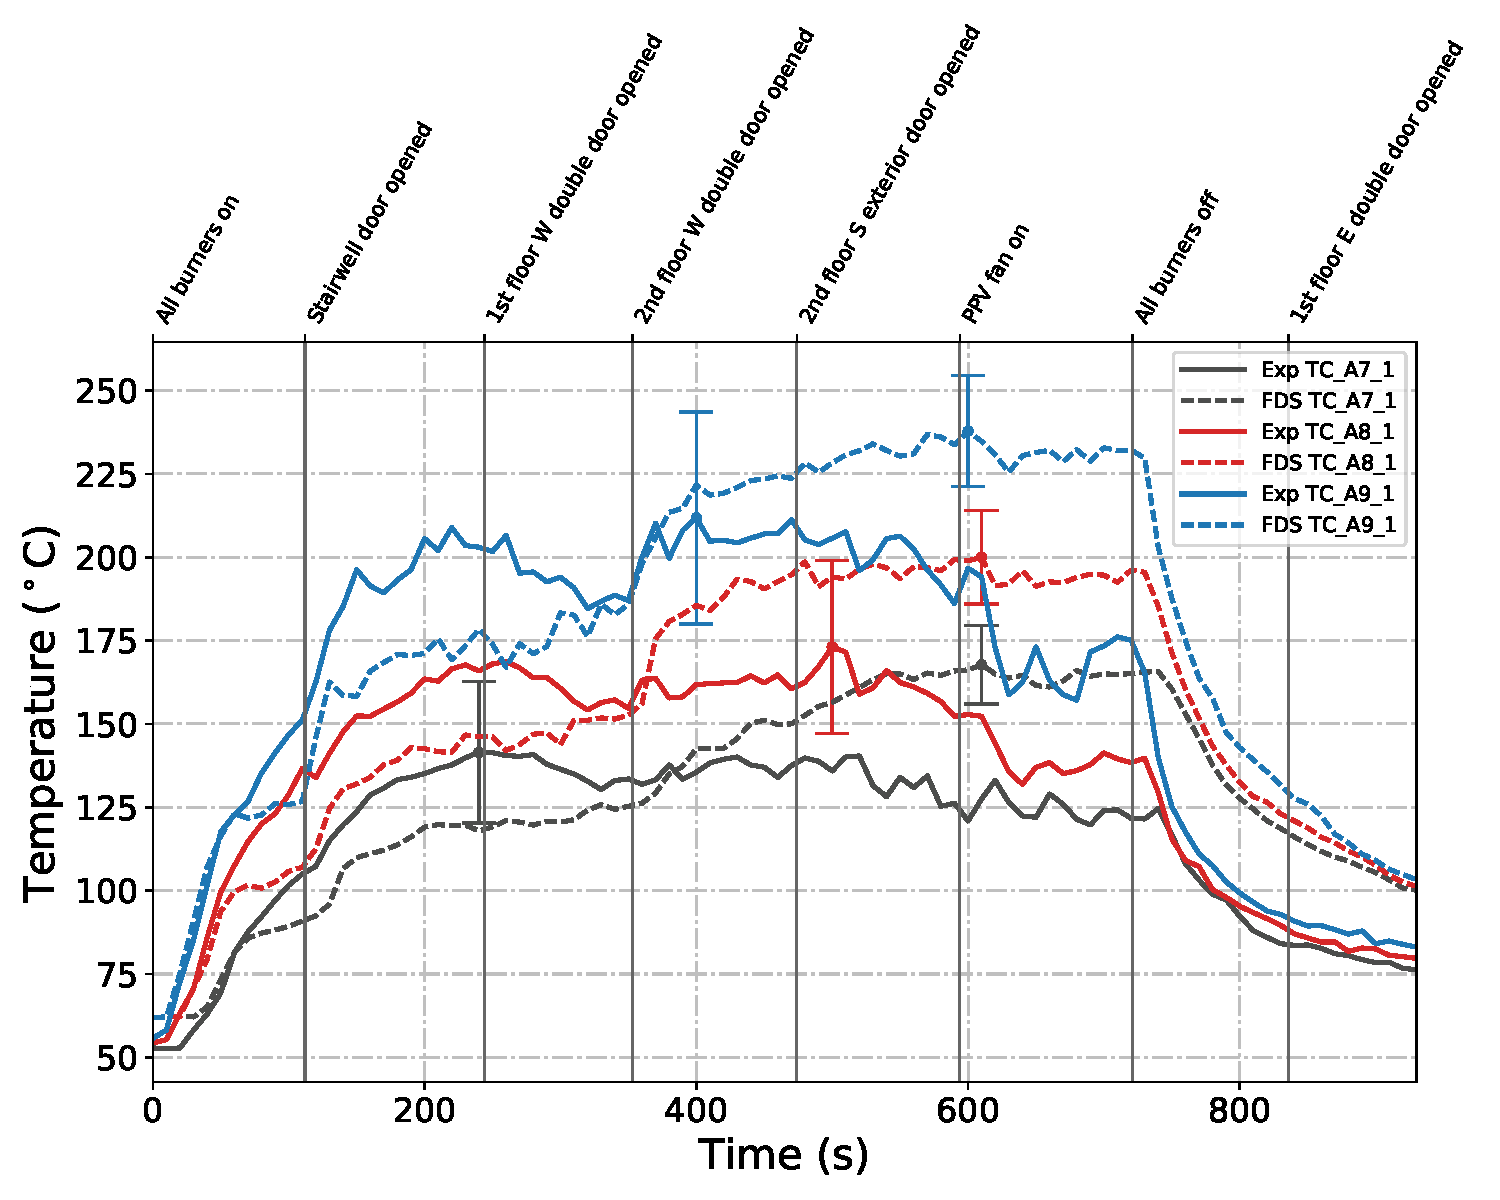
\includegraphics[width=\columnwidth]{Figures/Plots/Validation/Temperature/Test_25_cjet_2}
	\caption[Plots of measured and predicted ceiling jet temperatures on the second floor during Test~25.]{Plots of measured and predicted ceiling jet temperatures on the second floor of the West Structure during Test~25.}
	\label{fig:cjet2_data_Test25}
\end{figure}

\clearpage
\subsection*{\textit{Thermocouple Array Temperatures}}

\begin{figure}[!h]
	\centering
	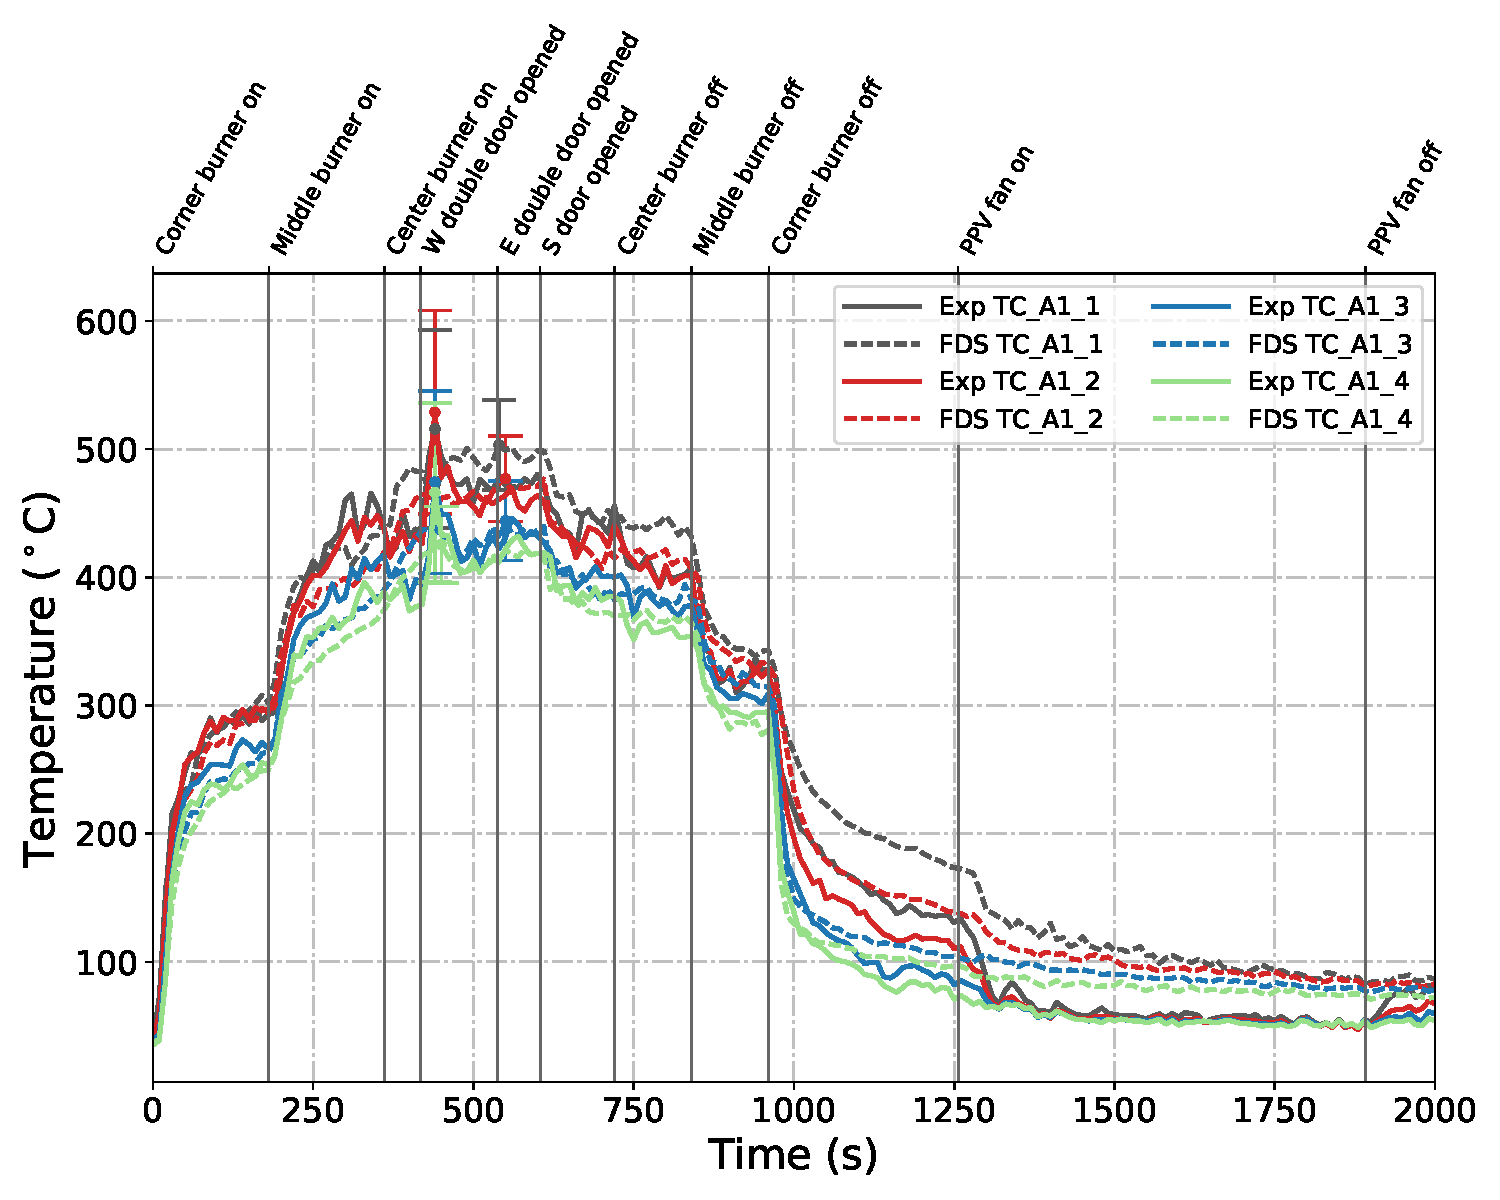
\includegraphics[width=\columnwidth]{Figures/Plots/Validation/Temperature/Test_2_TC_A1_upper}
	\caption{Plots of measured and predicted ``upper'' temperatures at array A1 during Test~2 in the East Structure.}
	\label{fig:TCA1_upper_data_Test2}
\end{figure}
\clearpage
\begin{figure}[!h]
	\centering
	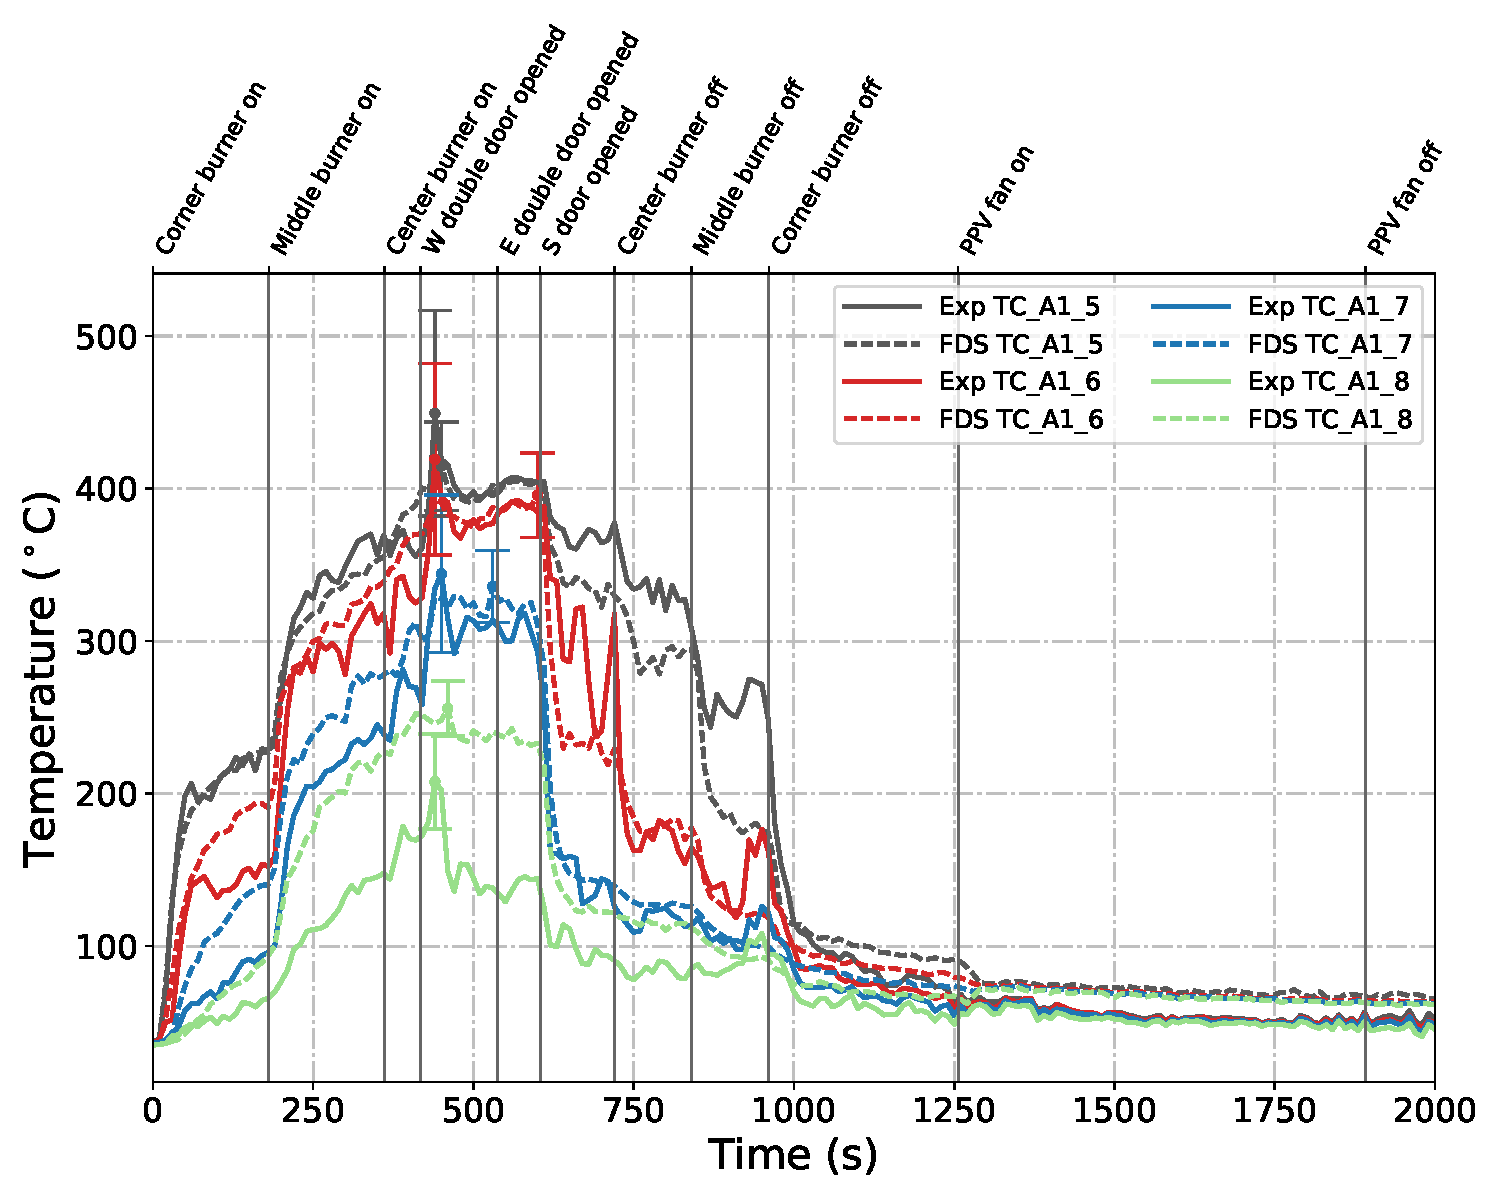
\includegraphics[width=\columnwidth]{Figures/Plots/Validation/Temperature/Test_2_TC_A1_lower}
	\caption{Plots of measured and predicted ``lower'' temperatures at array A1 during Test~2 in the East Structure.}
	\label{fig:TCA1_lower_data_Test2}
\end{figure}

\clearpage 

\begin{figure}[!h]
	\centering
	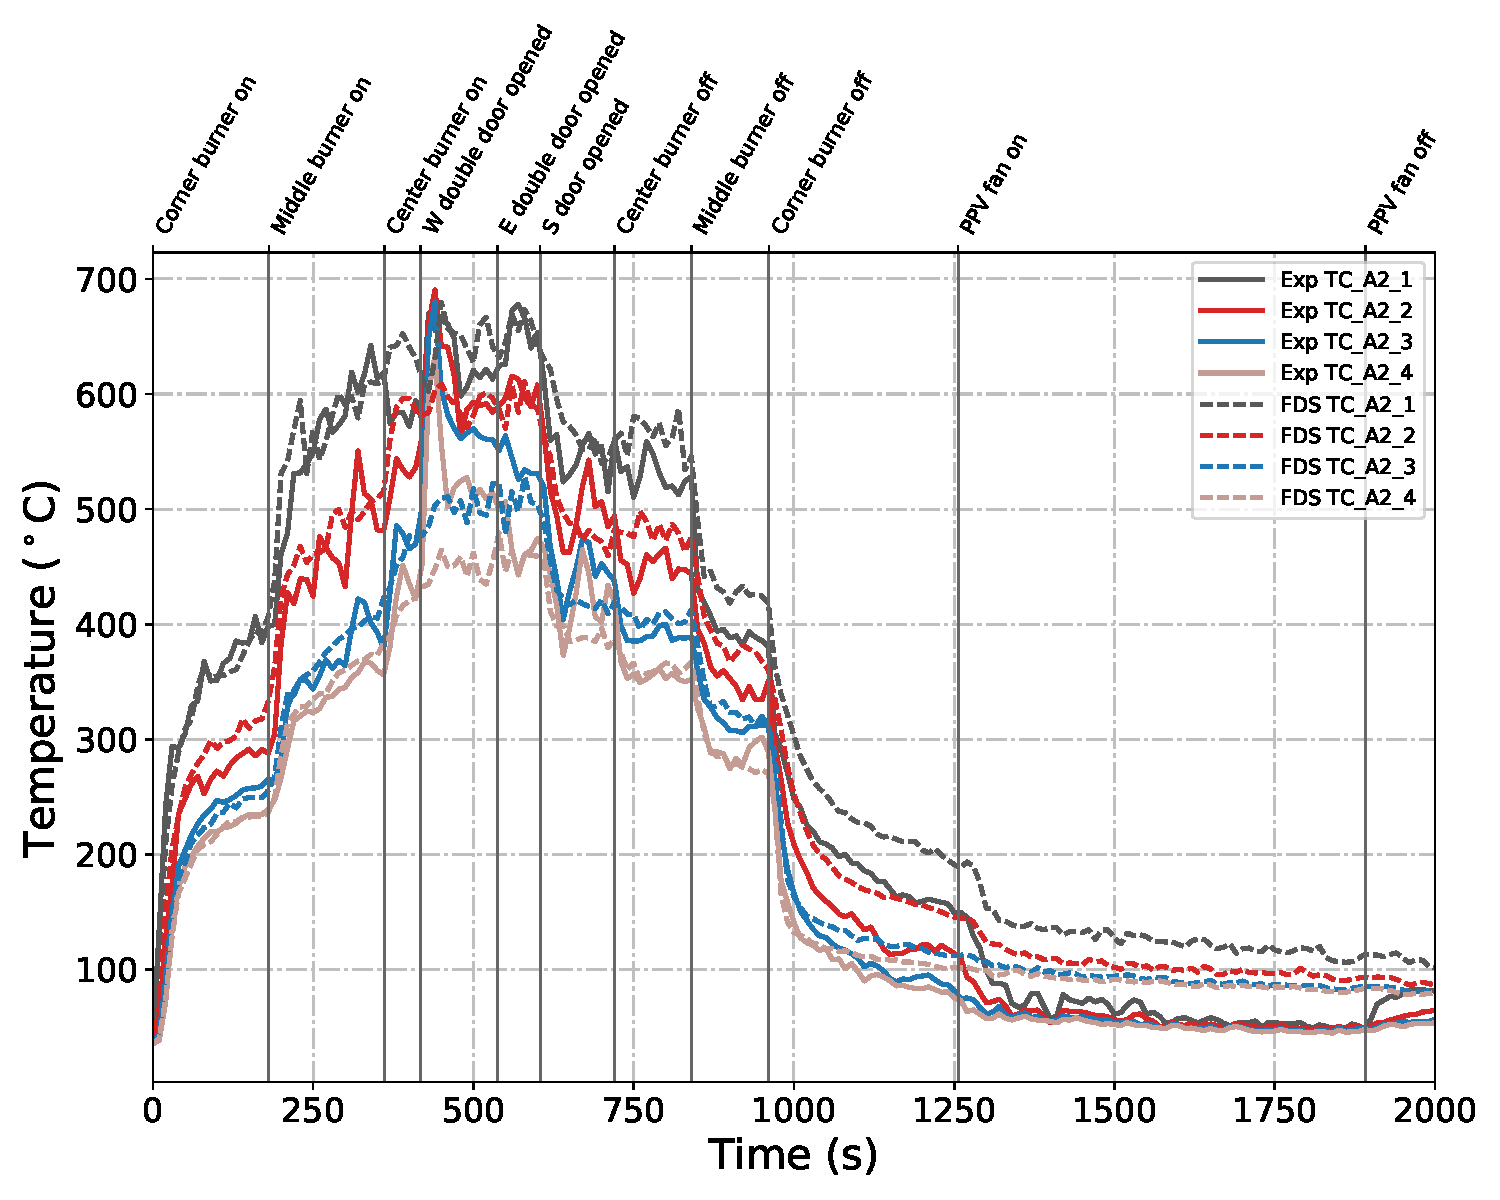
\includegraphics[width=\columnwidth]{Figures/Plots/Validation/Temperature/Test_2_TC_A2_upper}
	\caption{Plots of measured and predicted ``upper'' temperatures at array A2 during Test~2 in the East Structure.}
	\label{fig:TCA2_upper_data_Test2}
\end{figure}

\begin{figure}[!h]
	\centering
	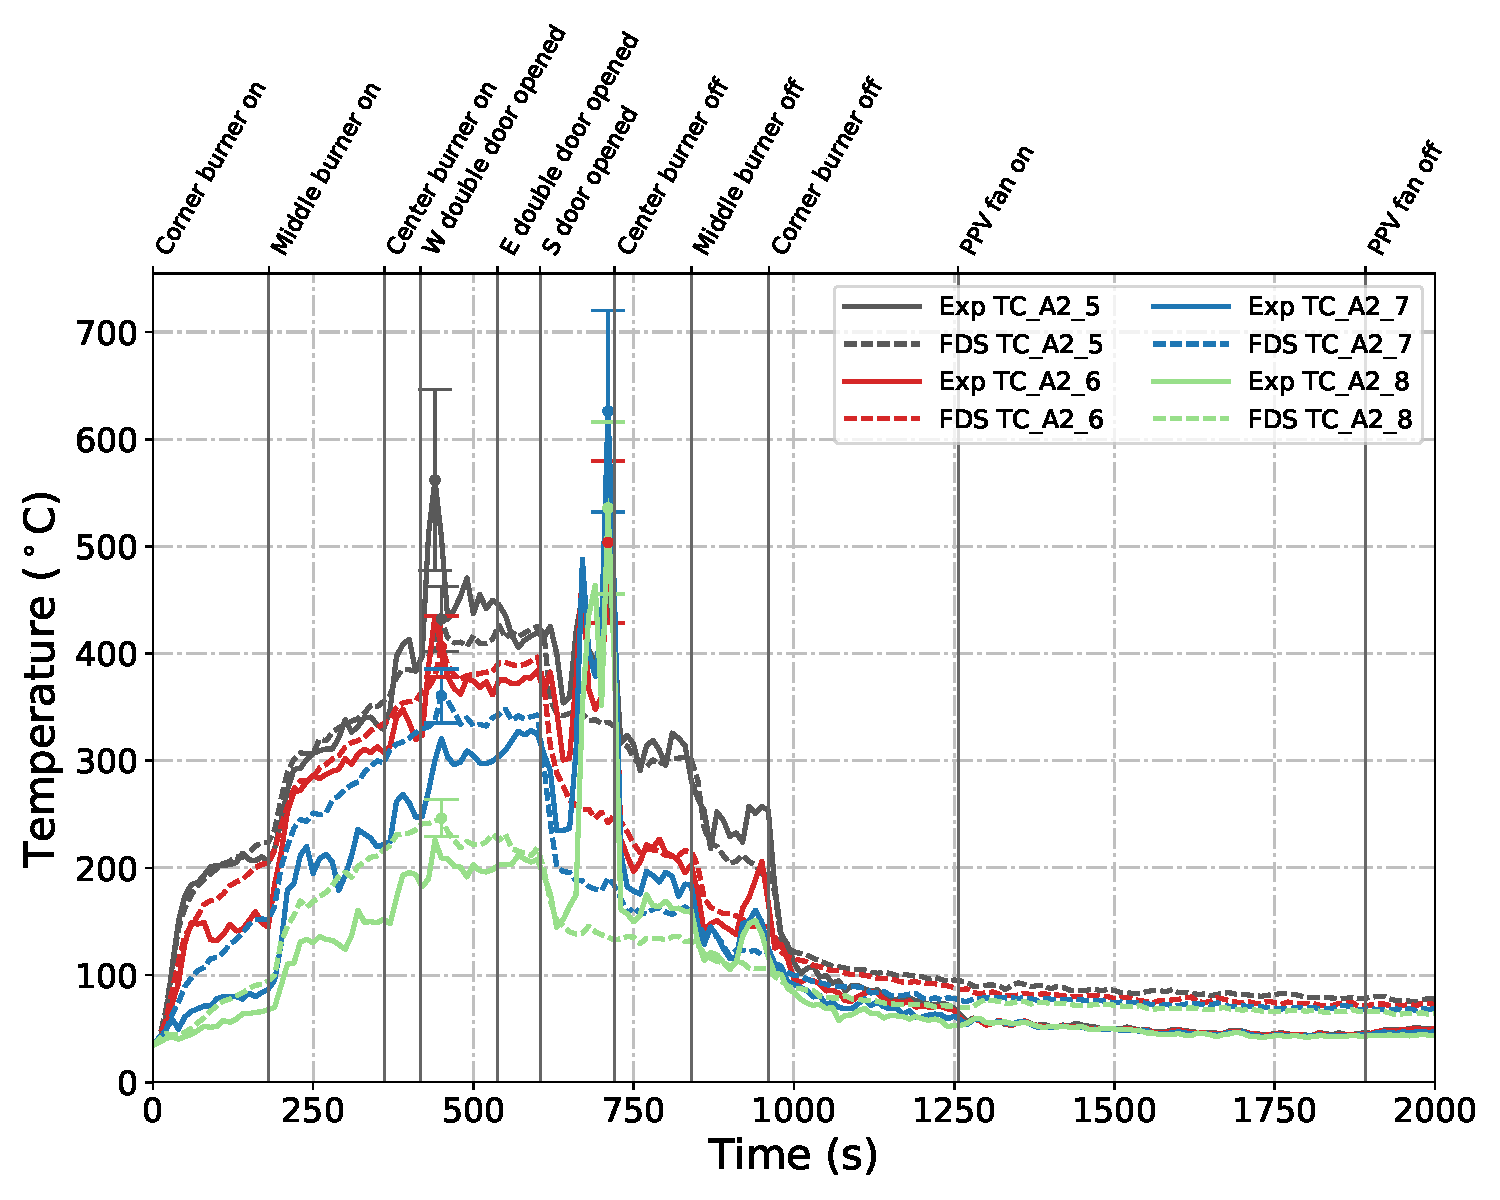
\includegraphics[width=\columnwidth]{Figures/Plots/Validation/Temperature/Test_2_TC_A2_lower}
	\caption{Plots of measured and predicted ``lower'' temperatures at array A2 during Test~2 in the East Structure.}
	\label{fig:TCA2_lower_data_Test2}
\end{figure}

% \begin{figure}[!h]
% 	\centering
% 	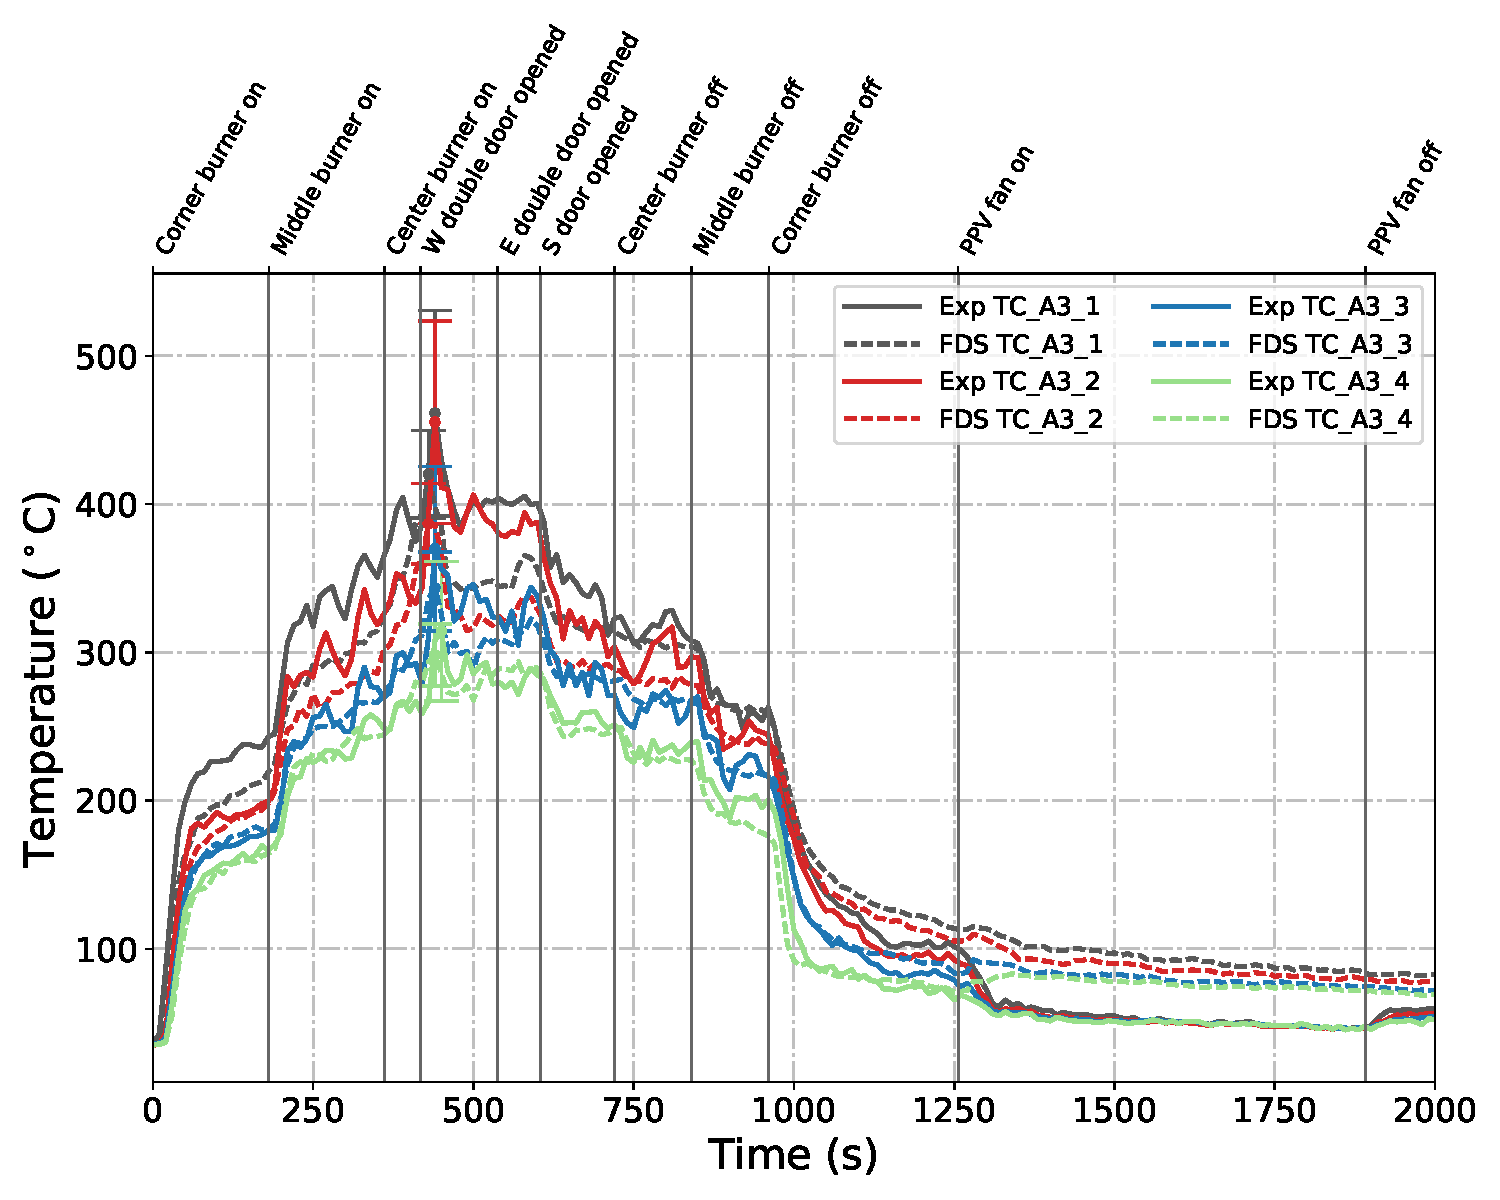
\includegraphics[width=\columnwidth]{Figures/Plots/Validation/Temperature/Test_2_TC_A3_upper}
% 	\caption{Plots of measured and predicted ``upper'' temperatures at array A3 during Test~2 in the East Structure.}
% 	\label{fig:TCA3_upper_data_Test2}
% \end{figure}

% \begin{figure}[!h]
% 	\centering
% 	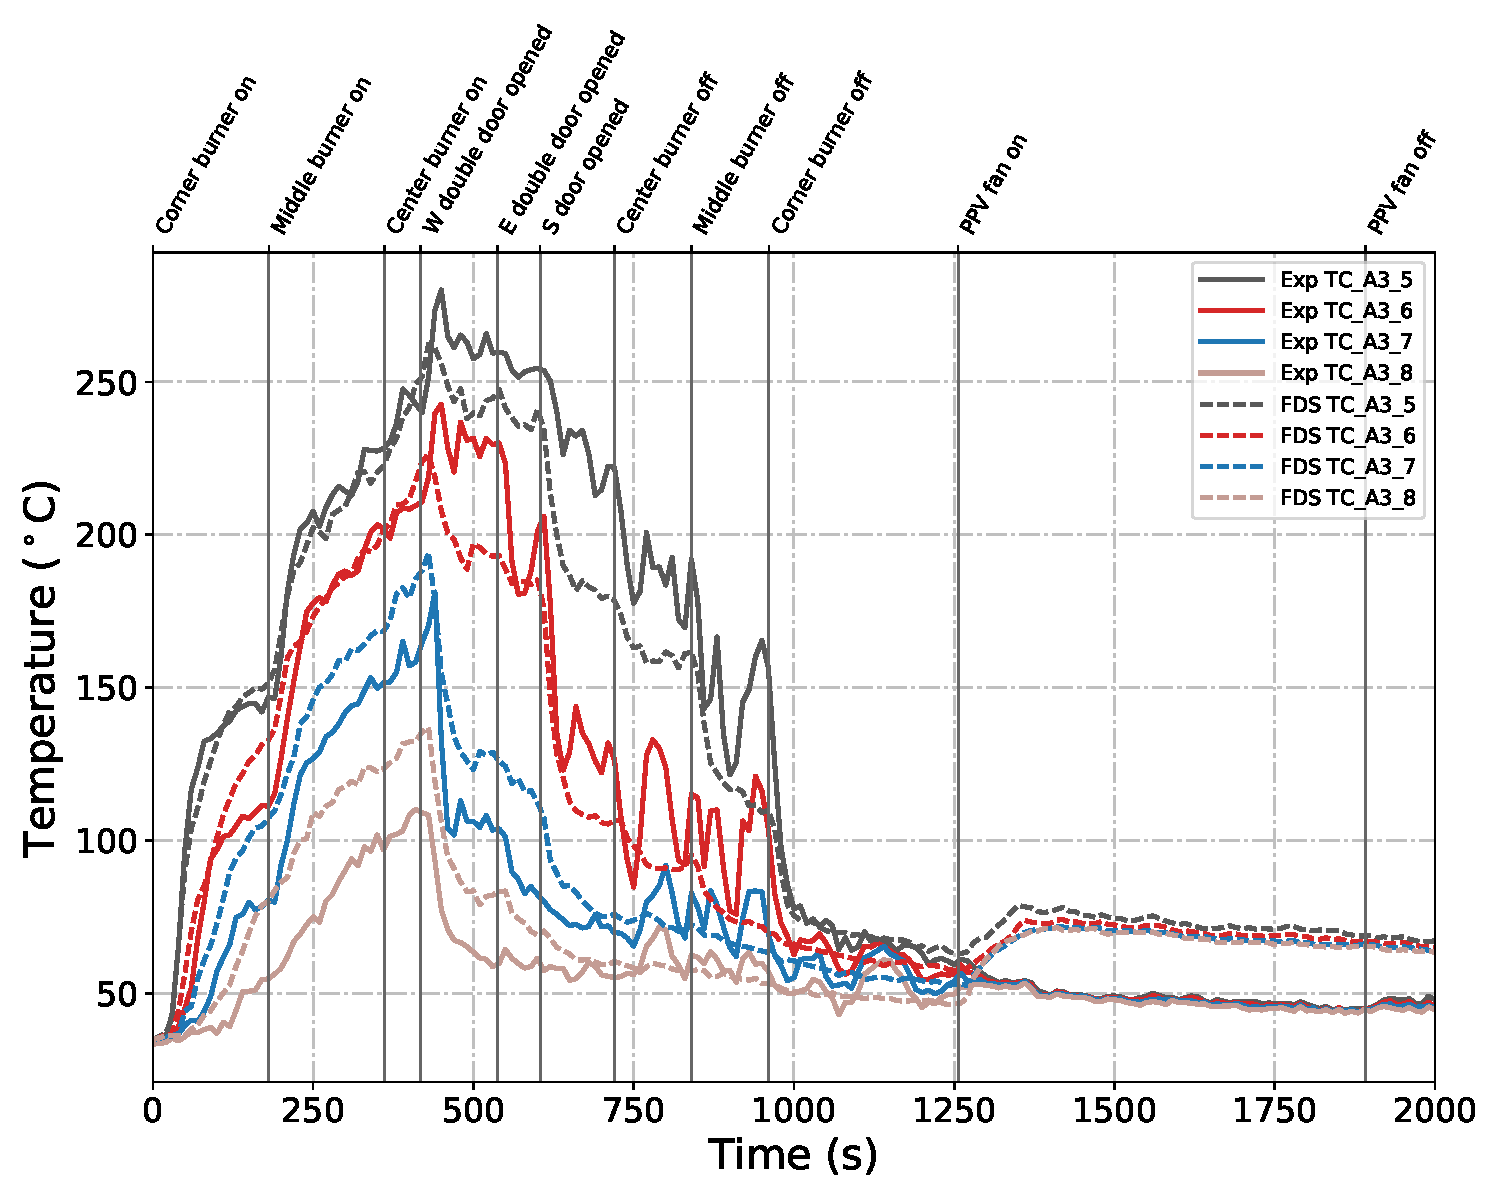
\includegraphics[width=\columnwidth]{Figures/Plots/Validation/Temperature/Test_2_TC_A3_lower}
% 	\caption{Plots of measured and predicted ``lower'' temperatures at array A3 during Test~2 in the East Structure.}
% 	\label{fig:TCA3_lower_data_Test2}
% \end{figure}

% \begin{figure}[!h]
% 	\centering
% 	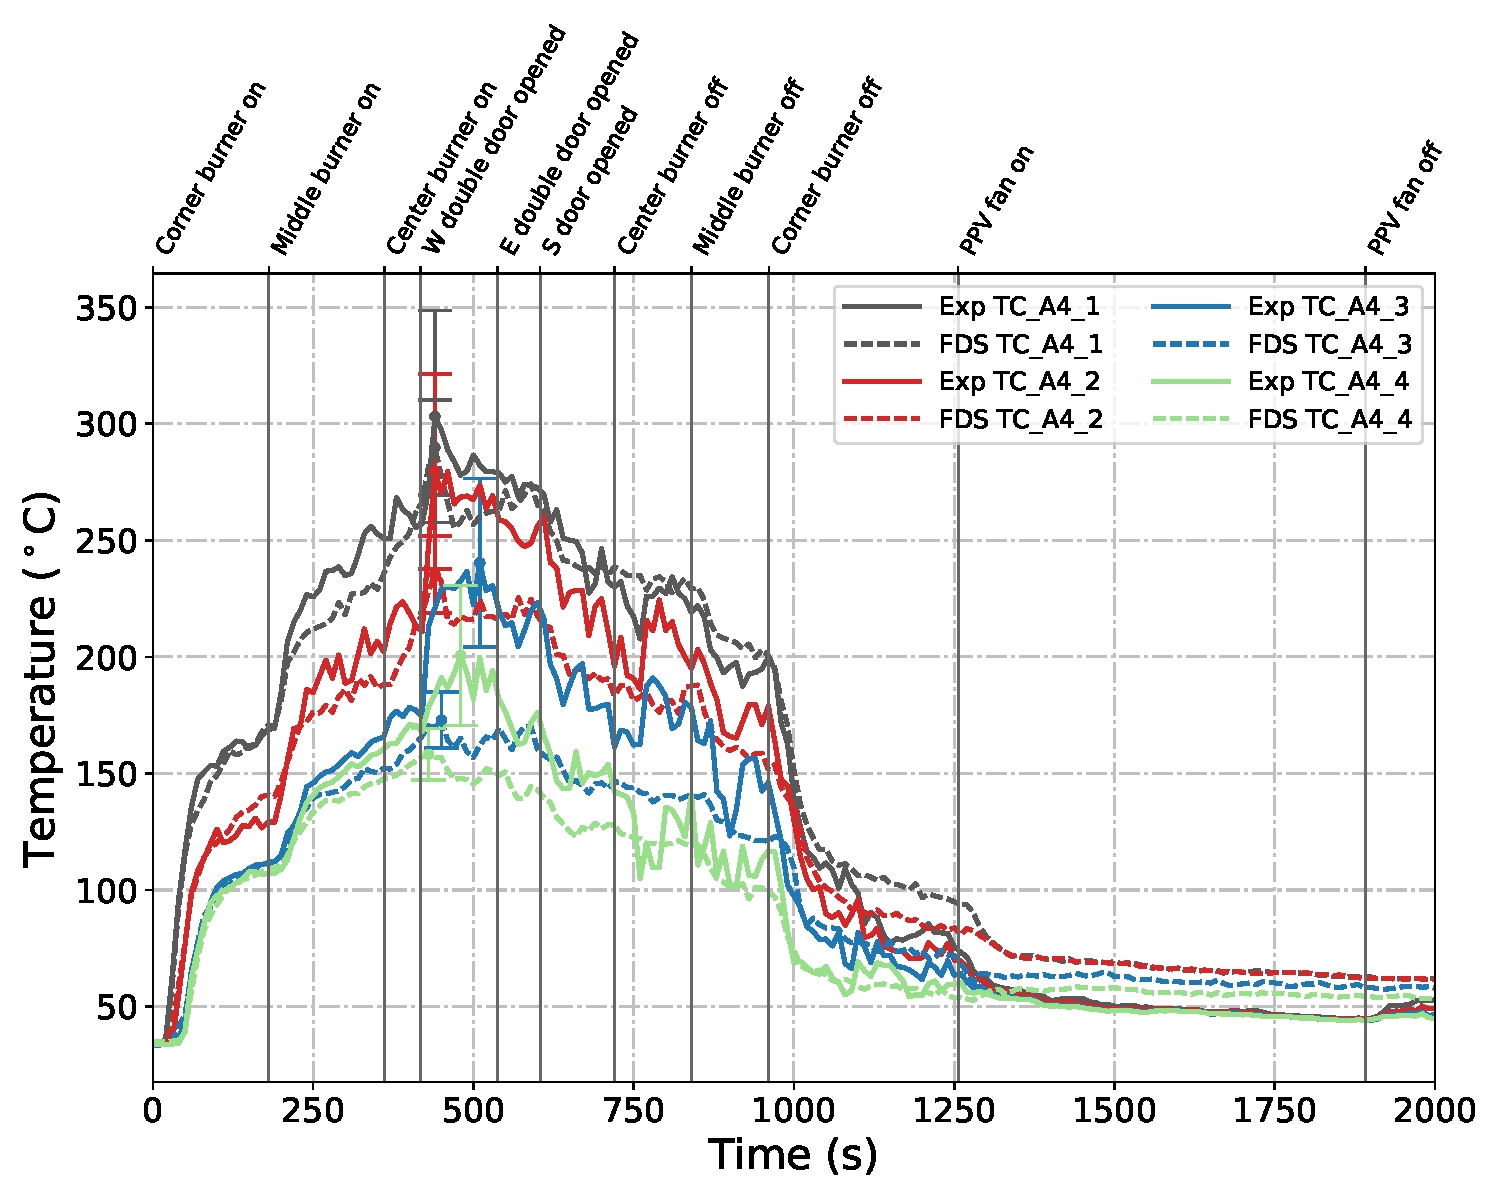
\includegraphics[width=\columnwidth]{Figures/Plots/Validation/Temperature/Test_2_TC_A4_upper}
% 	\caption{Plots of measured and predicted ``upper'' temperatures at array A4 during Test~2 in the East Structure.}
% 	\label{fig:TCA4_upper_data_Test2}
% \end{figure}

% \begin{figure}[!h]
% 	\centering
% 	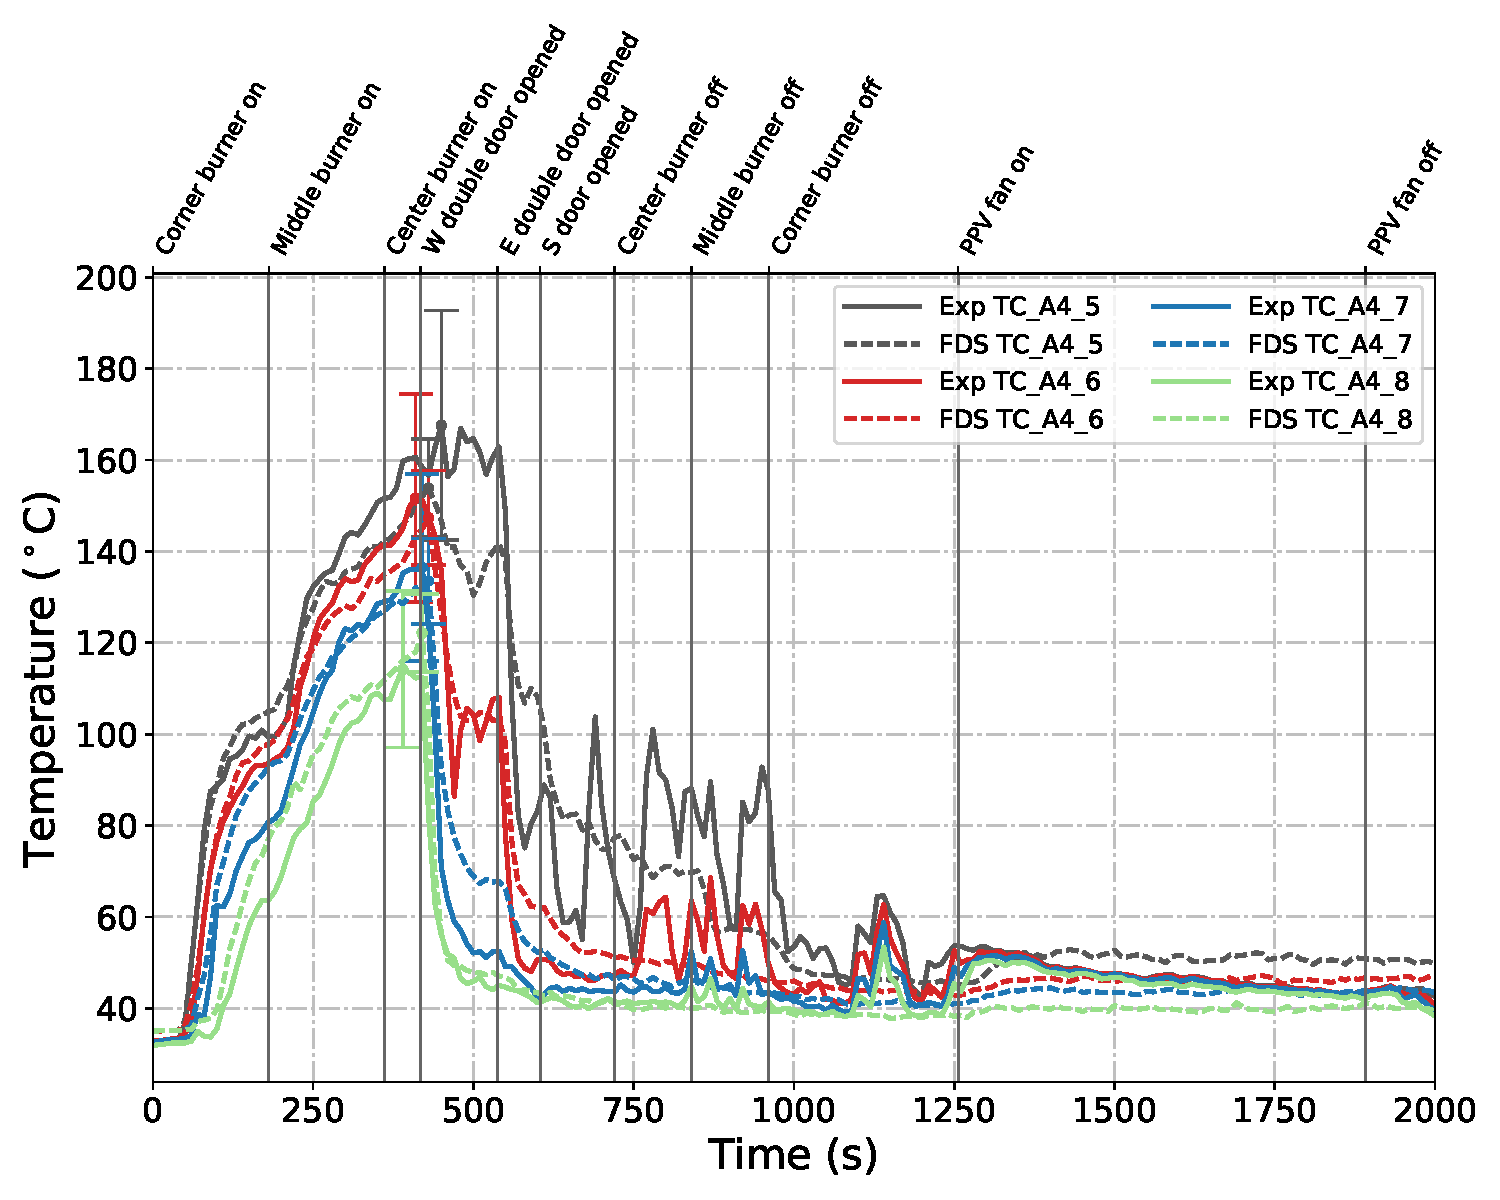
\includegraphics[width=\columnwidth]{Figures/Plots/Validation/Temperature/Test_2_TC_A4_lower}
% 	\caption{Plots of measured and predicted ``lower'' temperatures at array A4 during Test~2 in the East Structure.}
% 	\label{fig:TCA4_lower_data_Test2}
% \end{figure}

% \begin{figure}[!h]
% 	\centering
% 	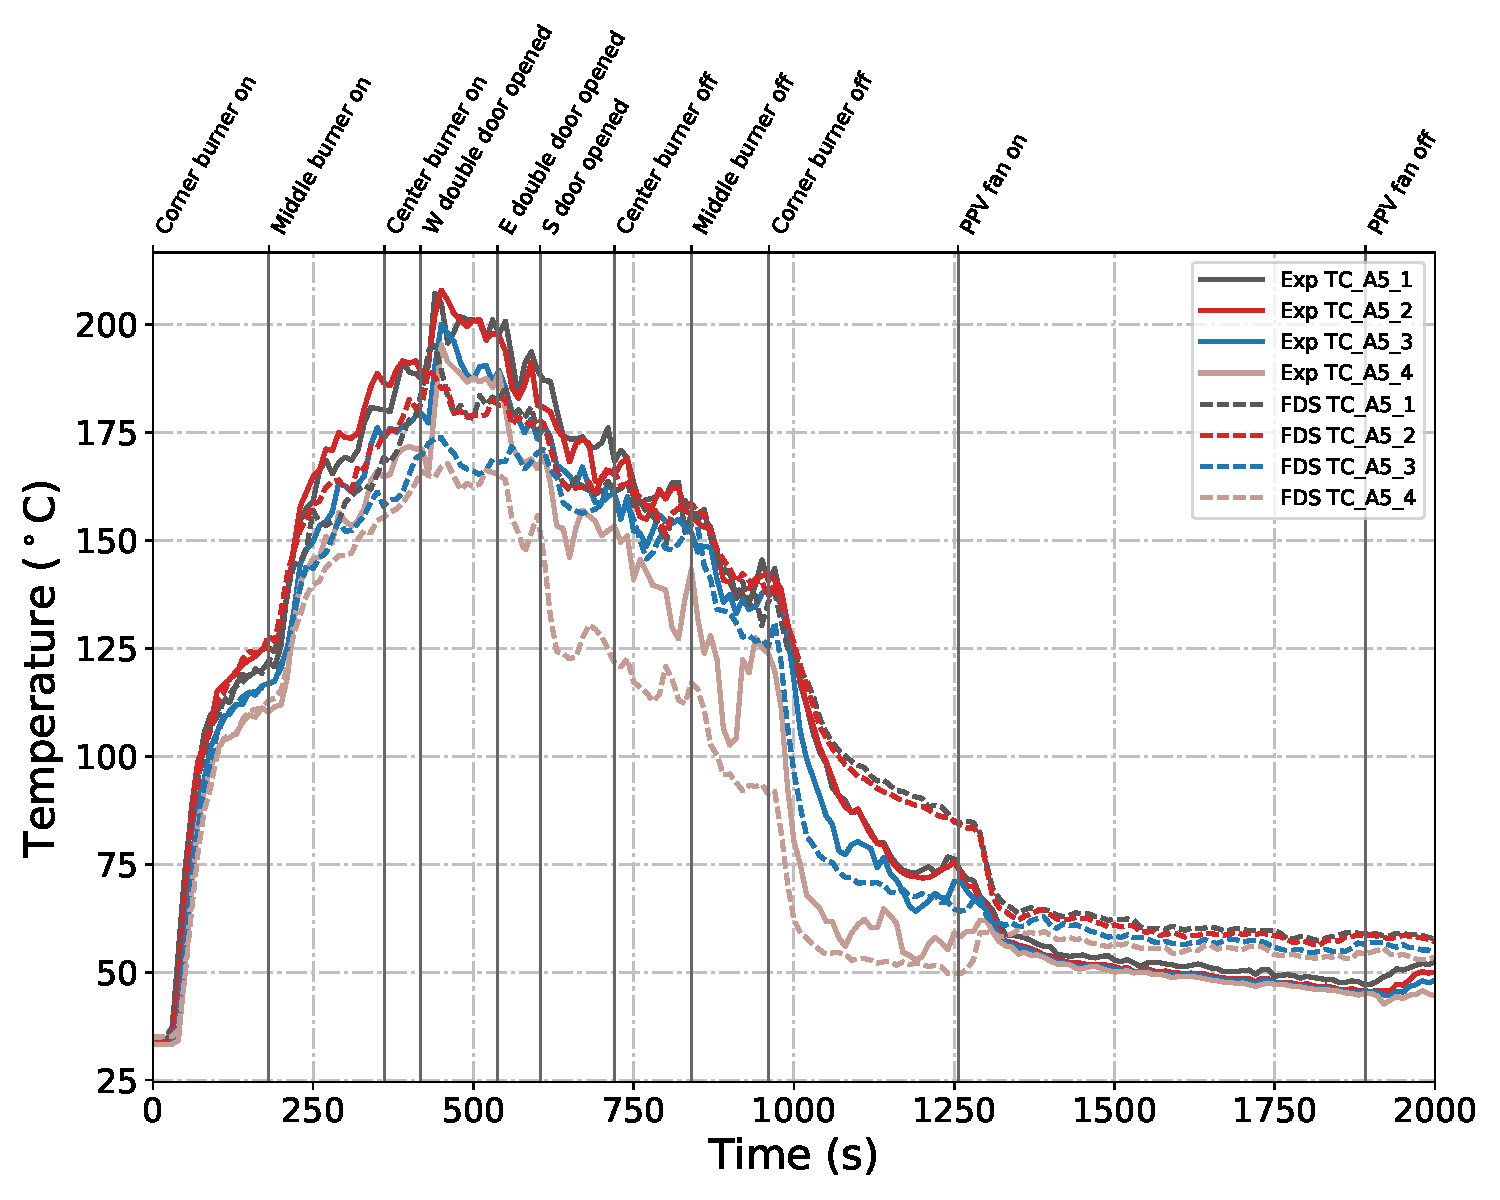
\includegraphics[width=\columnwidth]{Figures/Plots/Validation/Temperature/Test_2_TC_A5_upper}
% 	\caption{Plots of measured and predicted ``upper'' temperatures at array A5 during Test~2 in the East Structure.}
% 	\label{fig:TCA5_upper_data_Test2}
% \end{figure}

% \begin{figure}[!h]
% 	\centering
% 	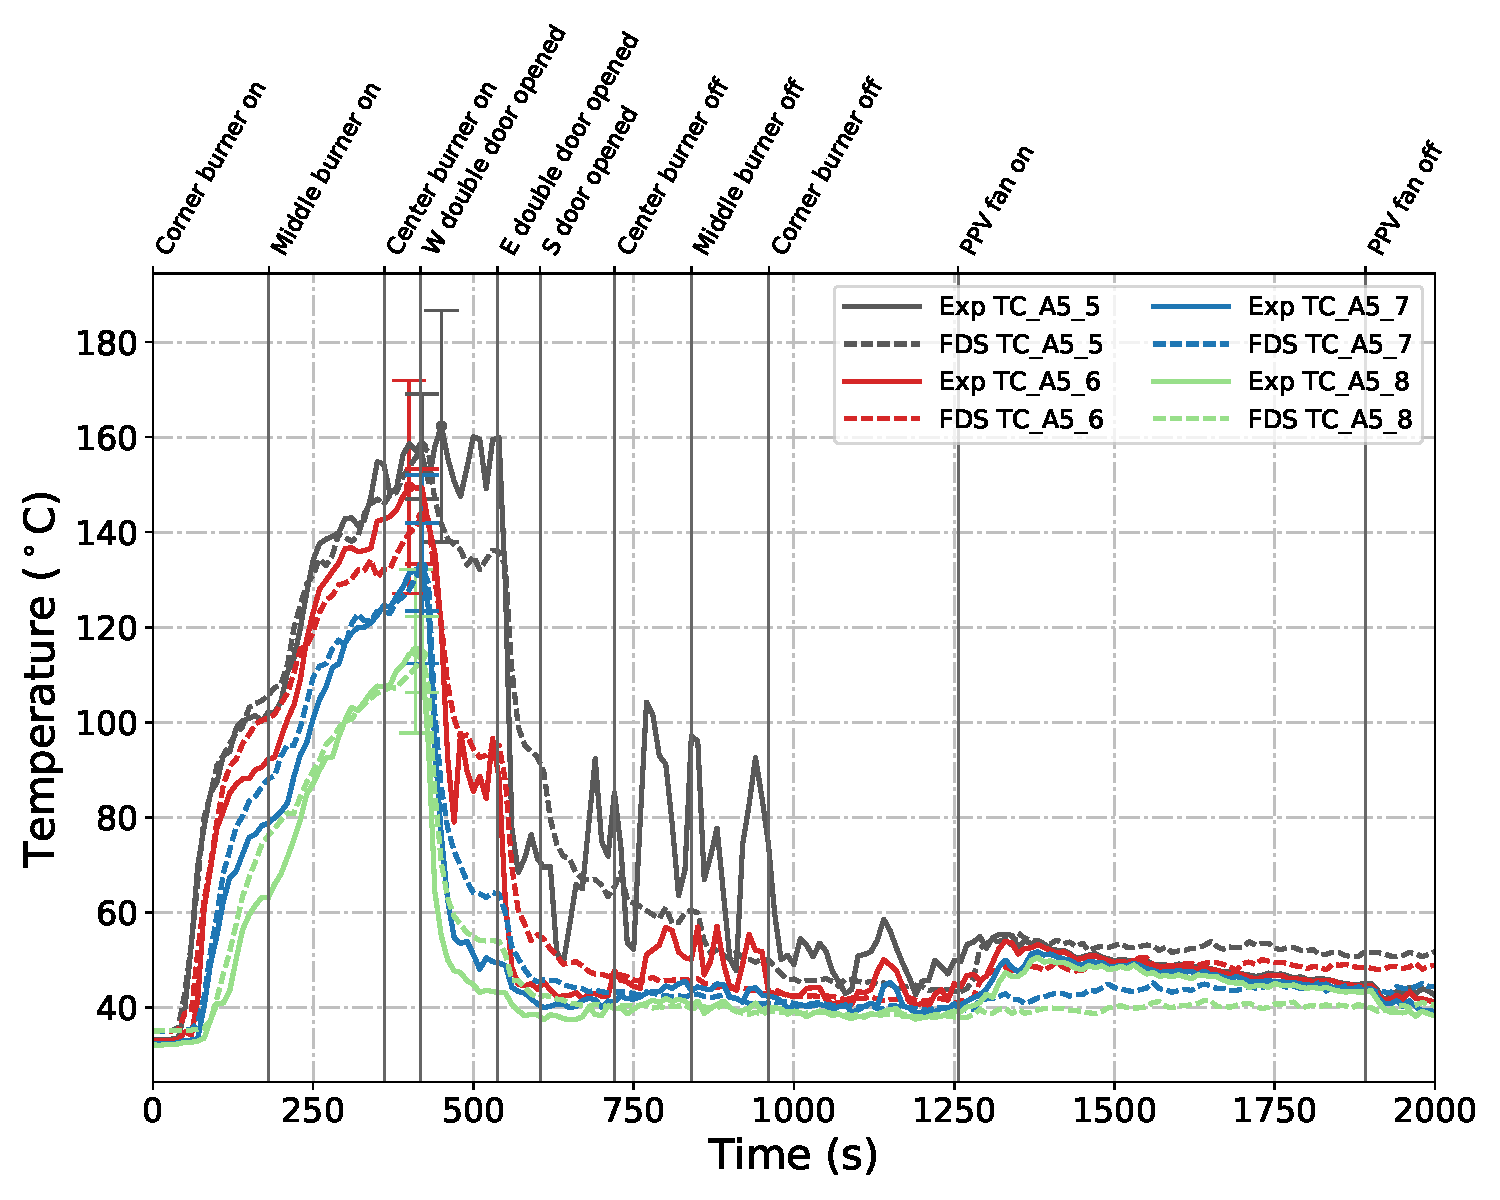
\includegraphics[width=\columnwidth]{Figures/Plots/Validation/Temperature/Test_2_TC_A5_lower}
% 	\caption{Plots of measured and predicted ``lower'' temperatures at array A5 during Test~2 in the East Structure.}
% 	\label{fig:TCA5_lower_data_Test2}
% \end{figure}

% \begin{figure}[!h]
% 	\centering
% 	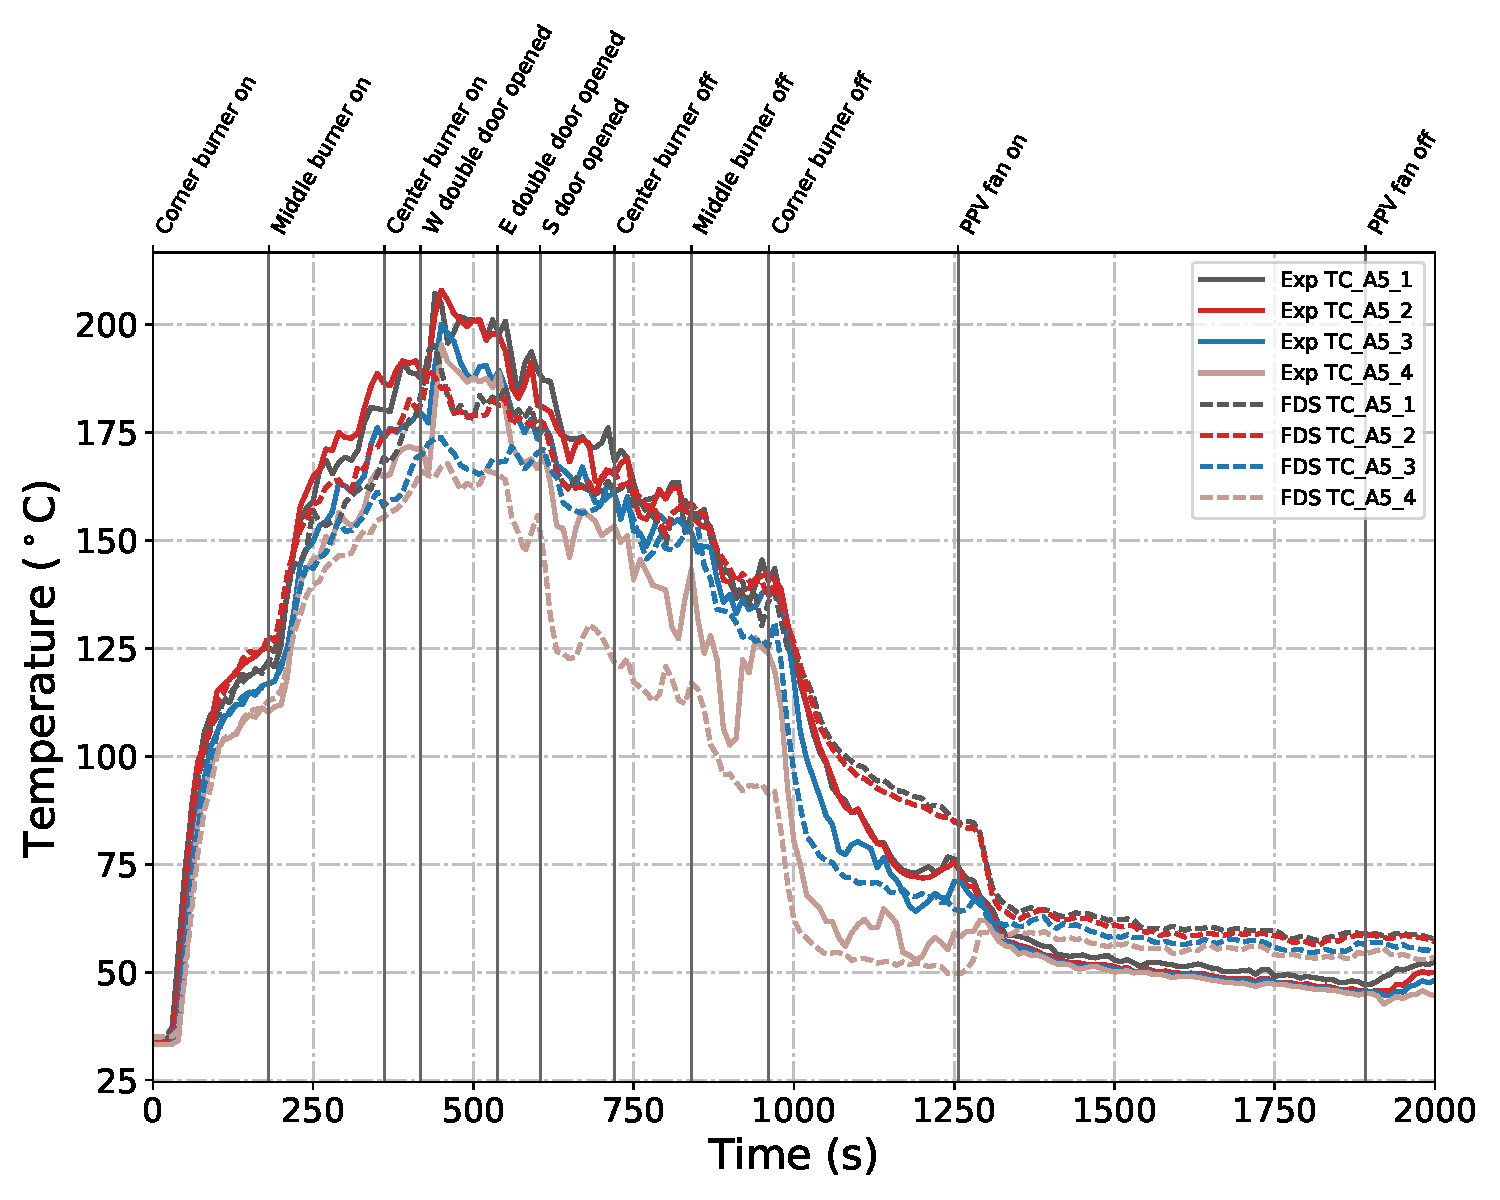
\includegraphics[width=\columnwidth]{Figures/Plots/Validation/Temperature/Test_2_TC_A5_upper}
% 	\caption{Plots of measured and predicted ``upper'' temperatures at array A5 during Test~2 in the East Structure.}
% 	\label{fig:TCA5_upper_data_Test2}
% \end{figure}

% \begin{figure}[!h]
% 	\centering
% 	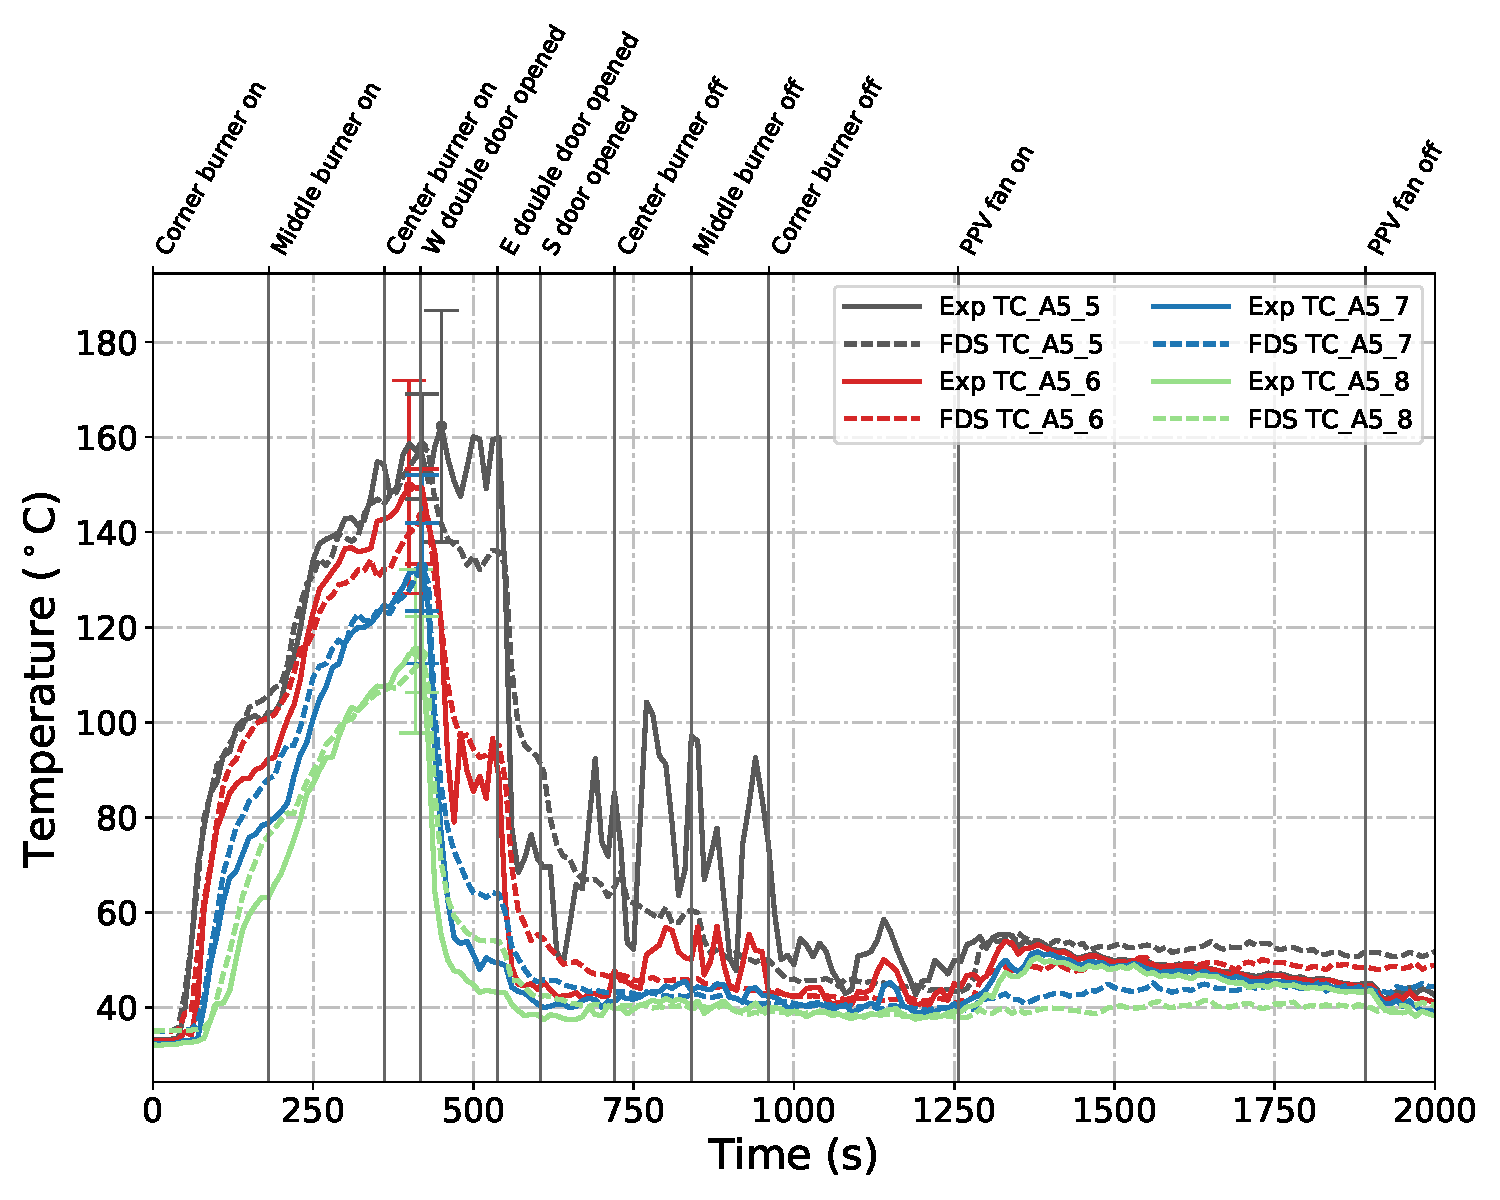
\includegraphics[width=\columnwidth]{Figures/Plots/Validation/Temperature/Test_2_TC_A5_lower}
% 	\caption{Plots of measured and predicted ``lower'' temperatures at array A5 during Test~2 in the East Structure.}
% 	\label{fig:TCA5_lower_data_Test2}
% \end{figure}

% %%%%%%%%%%%%%%%%%%%%%%%%%%%%%%%%%%%%%%%%
% \begin{figure}[!h]
% 	\centering
% 	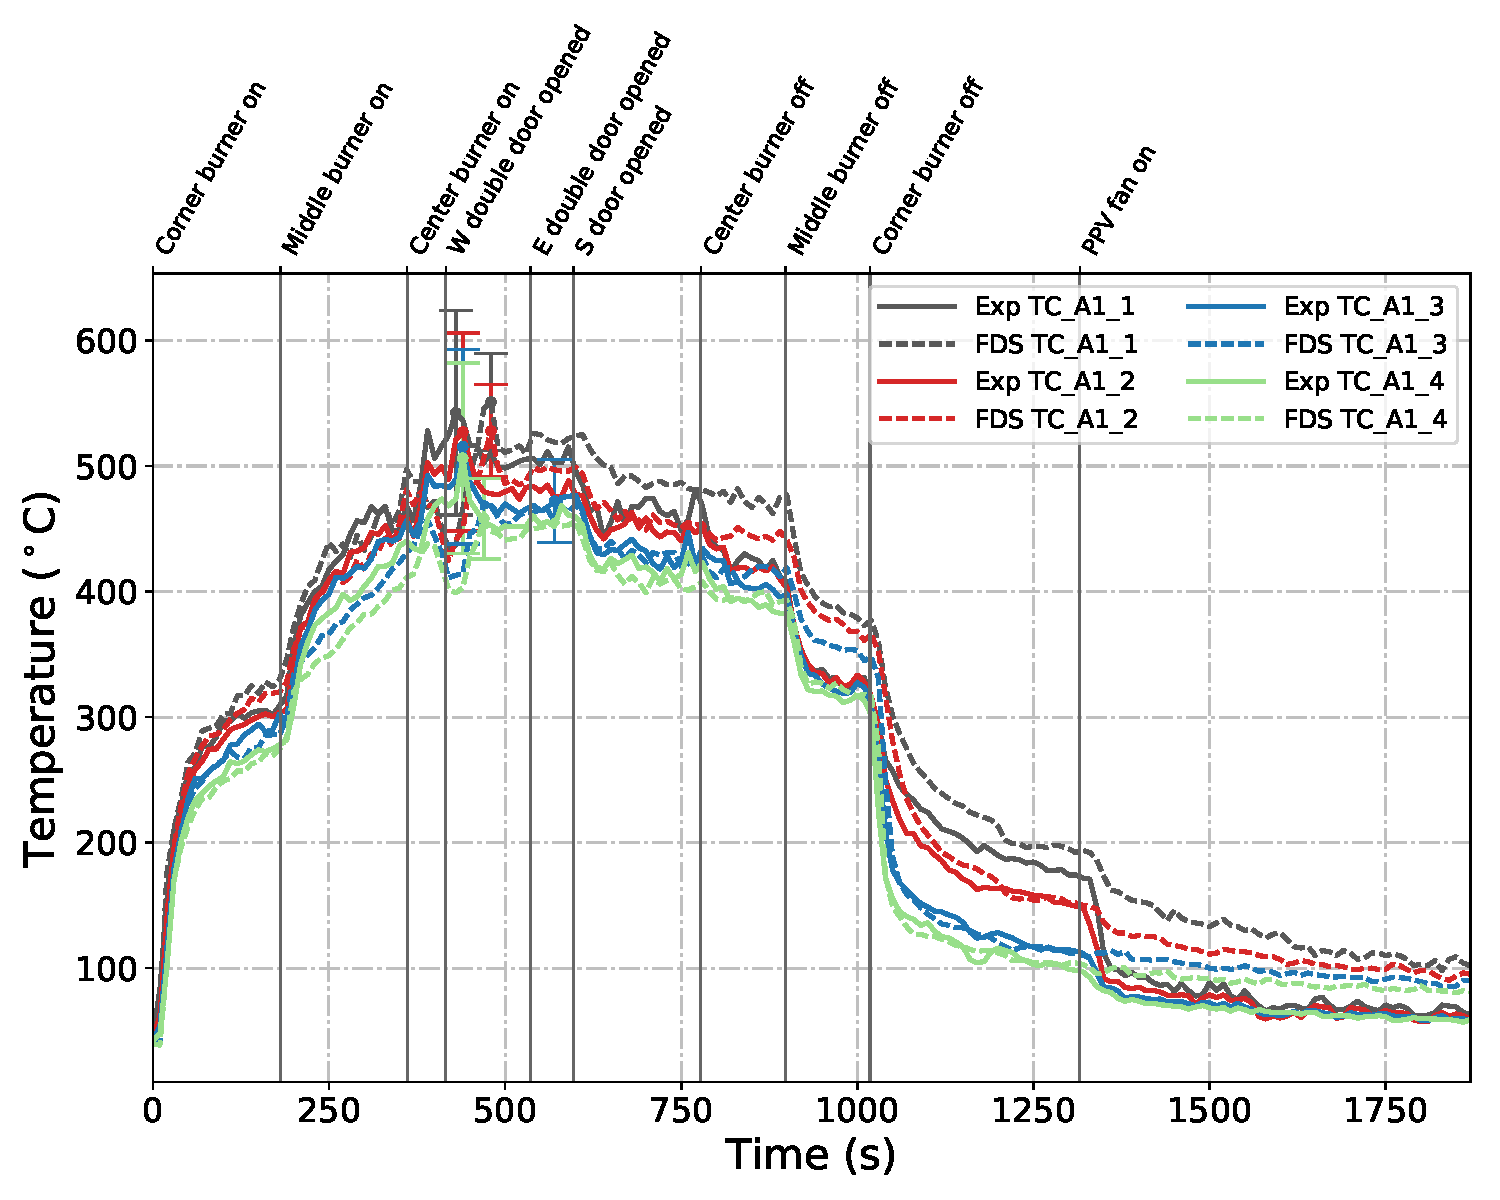
\includegraphics[width=\columnwidth]{Figures/Plots/Validation/Temperature/Test_3_TC_A1_upper}
% 	\caption{Plots of measured and predicted ``upper'' temperatures at array A1 during Test~3 in the East Structure.}
% 	\label{fig:TCA1_upper_data_Test3}
% \end{figure}

% \begin{figure}[!h]
% 	\centering
% 	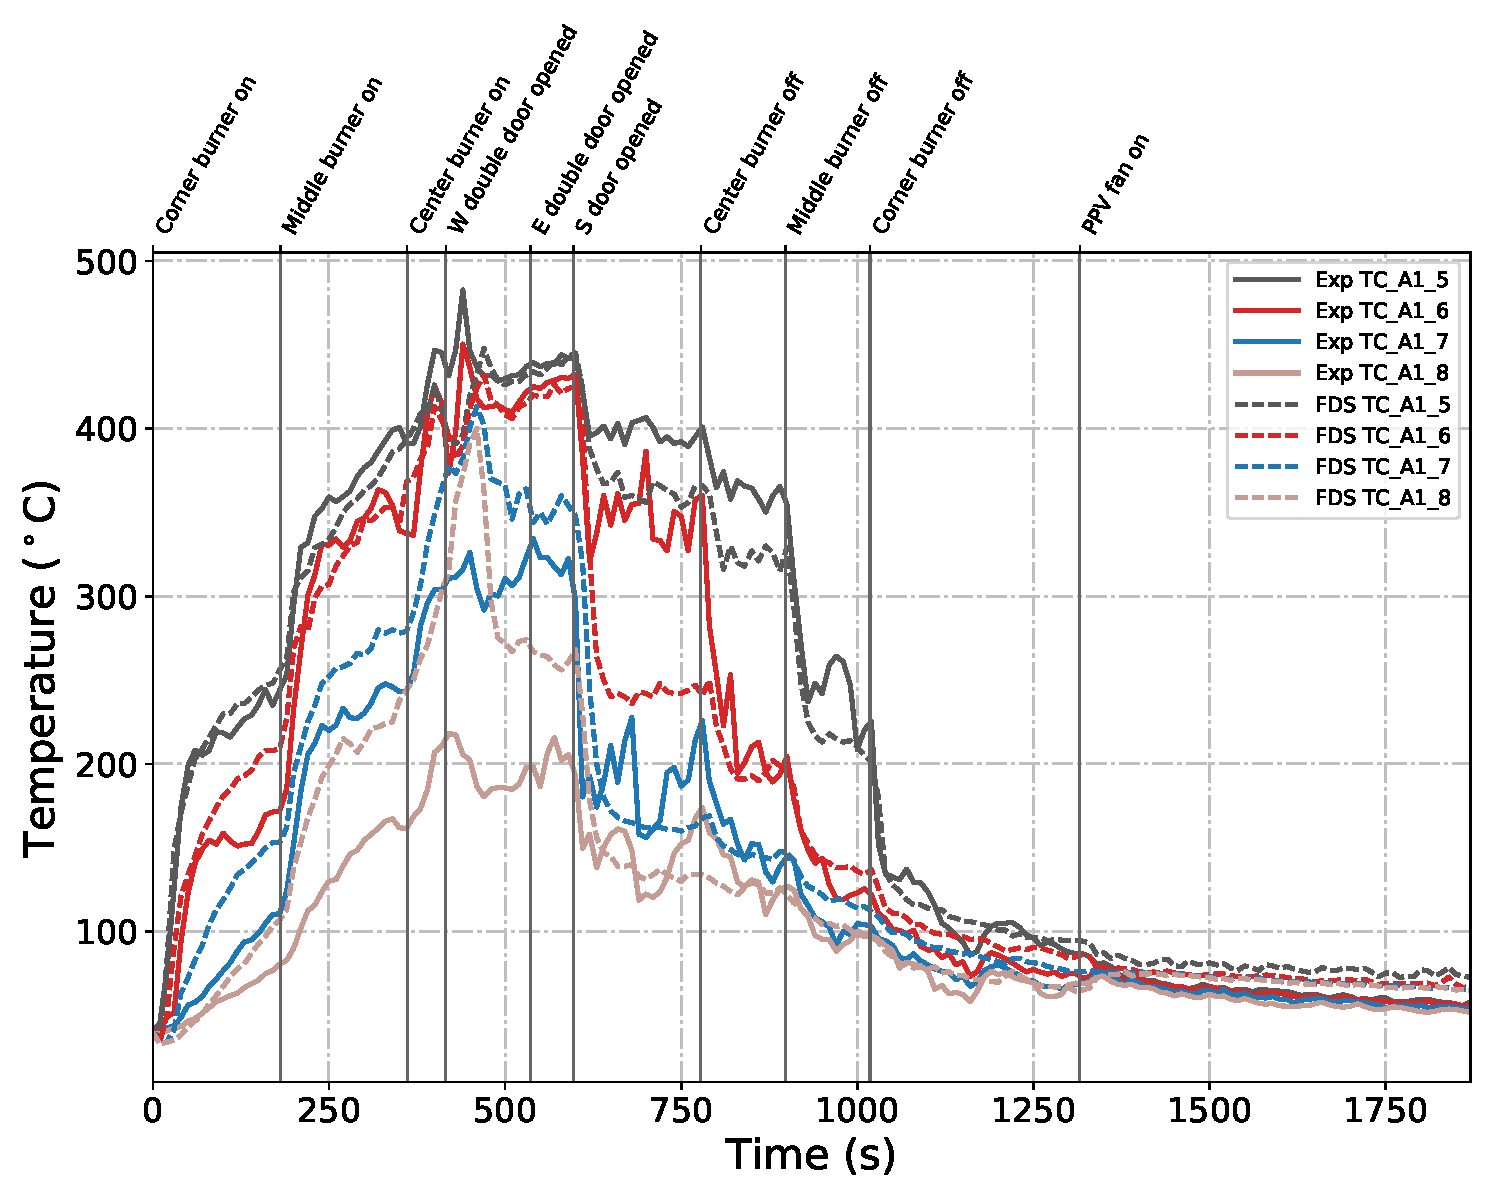
\includegraphics[width=\columnwidth]{Figures/Plots/Validation/Temperature/Test_3_TC_A1_lower}
% 	\caption{Plots of measured and predicted ``lower'' temperatures at array A1 during Test~3 in the East Structure.}
% 	\label{fig:TCA1_lower_data_Test3}
% \end{figure}

% \begin{figure}[!h]
% 	\centering
% 	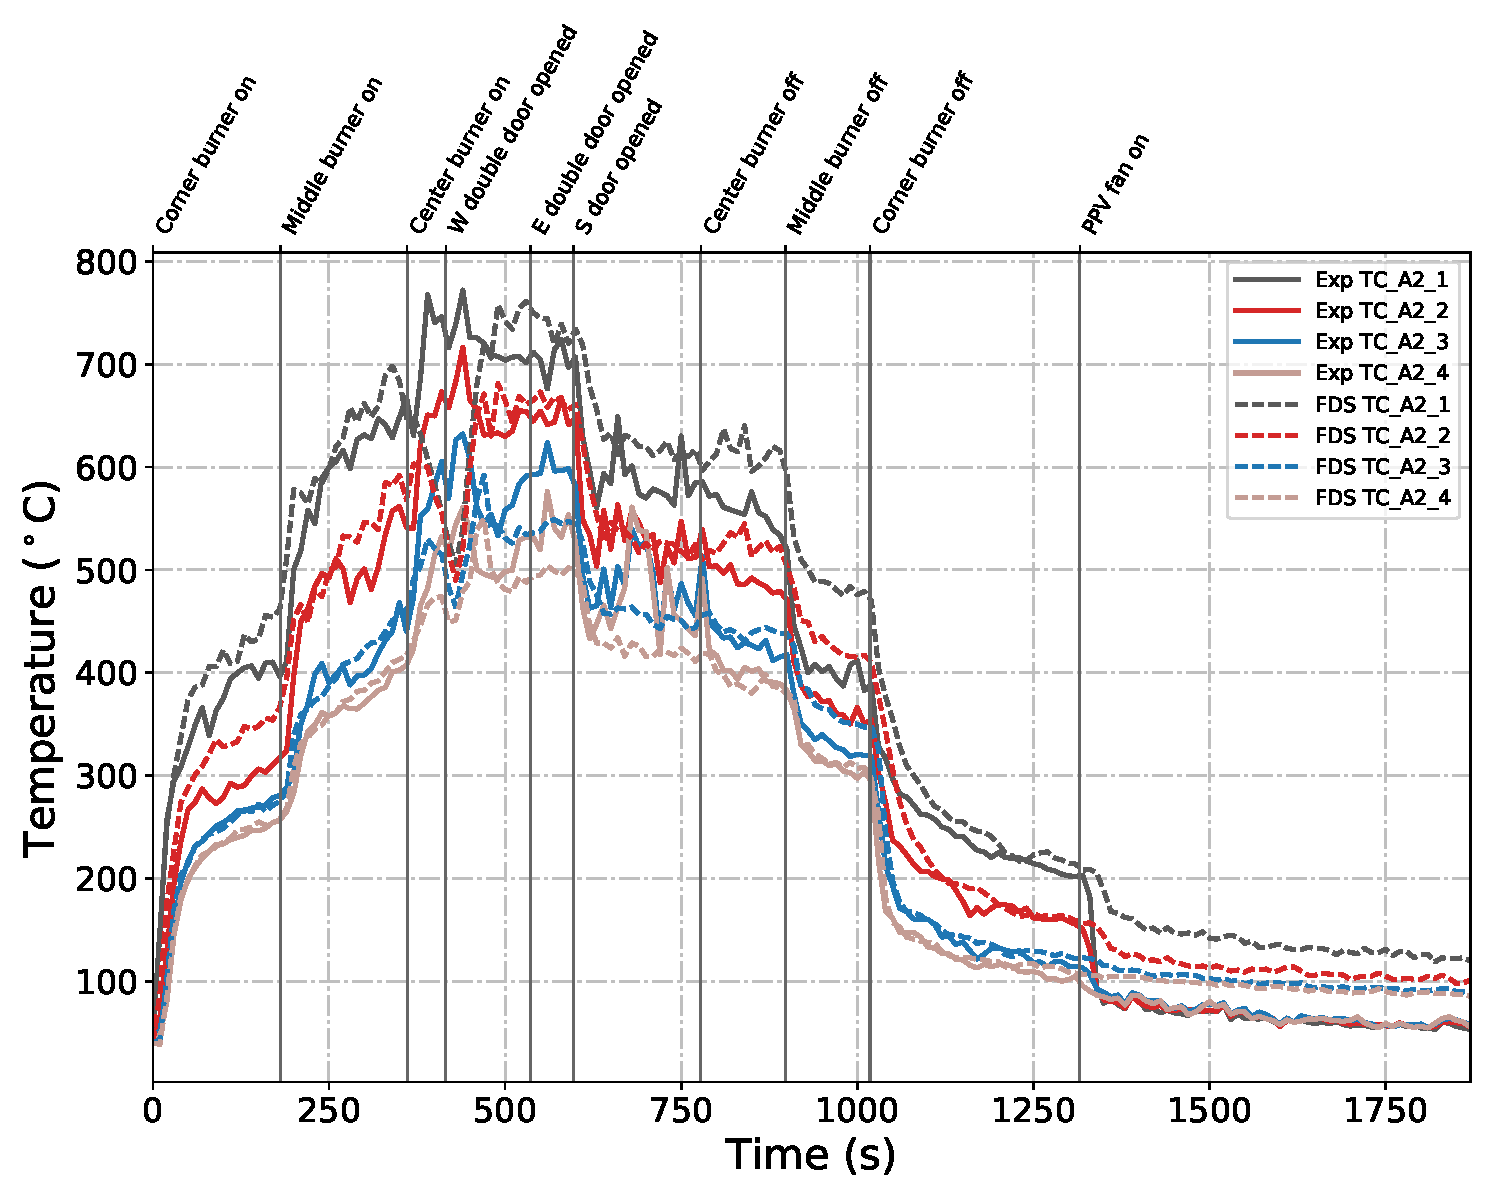
\includegraphics[width=\columnwidth]{Figures/Plots/Validation/Temperature/Test_3_TC_A2_upper}
% 	\caption{Plots of measured and predicted ``upper'' temperatures at array A2 during Test~3 in the East Structure.}
% 	\label{fig:TCA2_upper_data_Test3}
% \end{figure}

% \begin{figure}[!h]
% 	\centering
% 	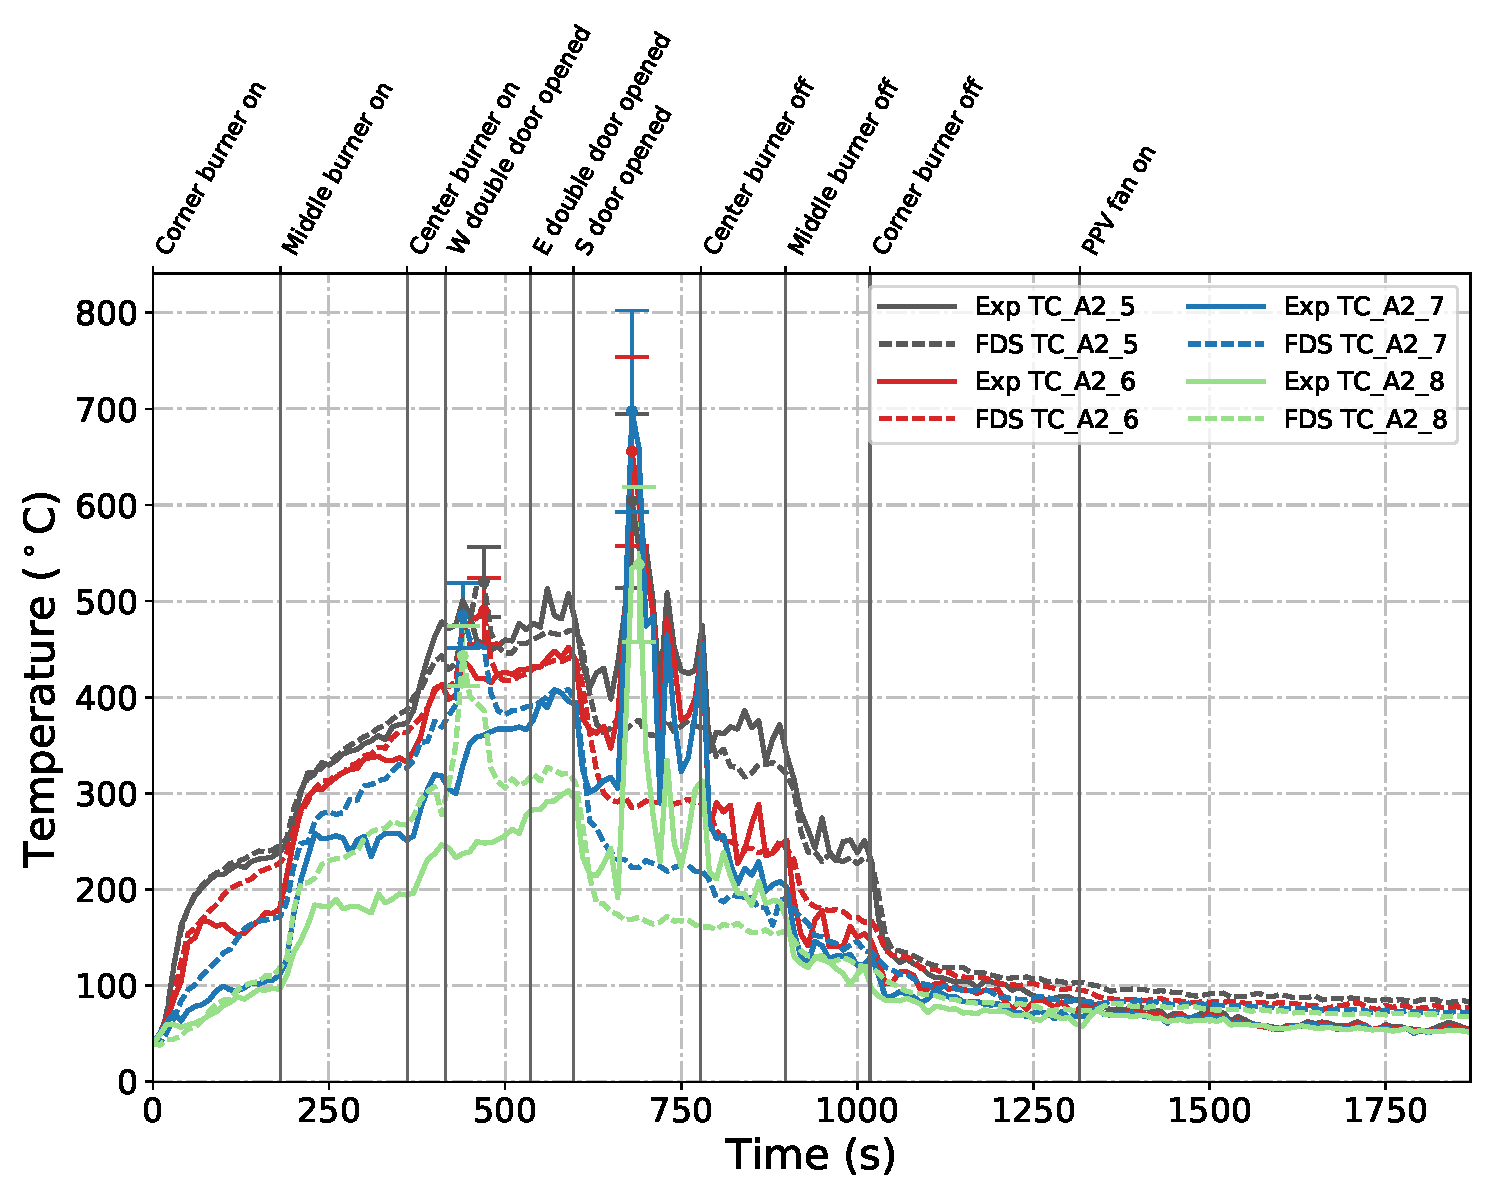
\includegraphics[width=\columnwidth]{Figures/Plots/Validation/Temperature/Test_3_TC_A2_lower}
% 	\caption{Plots of measured and predicted ``lower'' temperatures at array A2 during Test~3 in the East Structure.}
% 	\label{fig:TCA2_lower_data_Test3}
% \end{figure}

% \begin{figure}[!h]
% 	\centering
% 	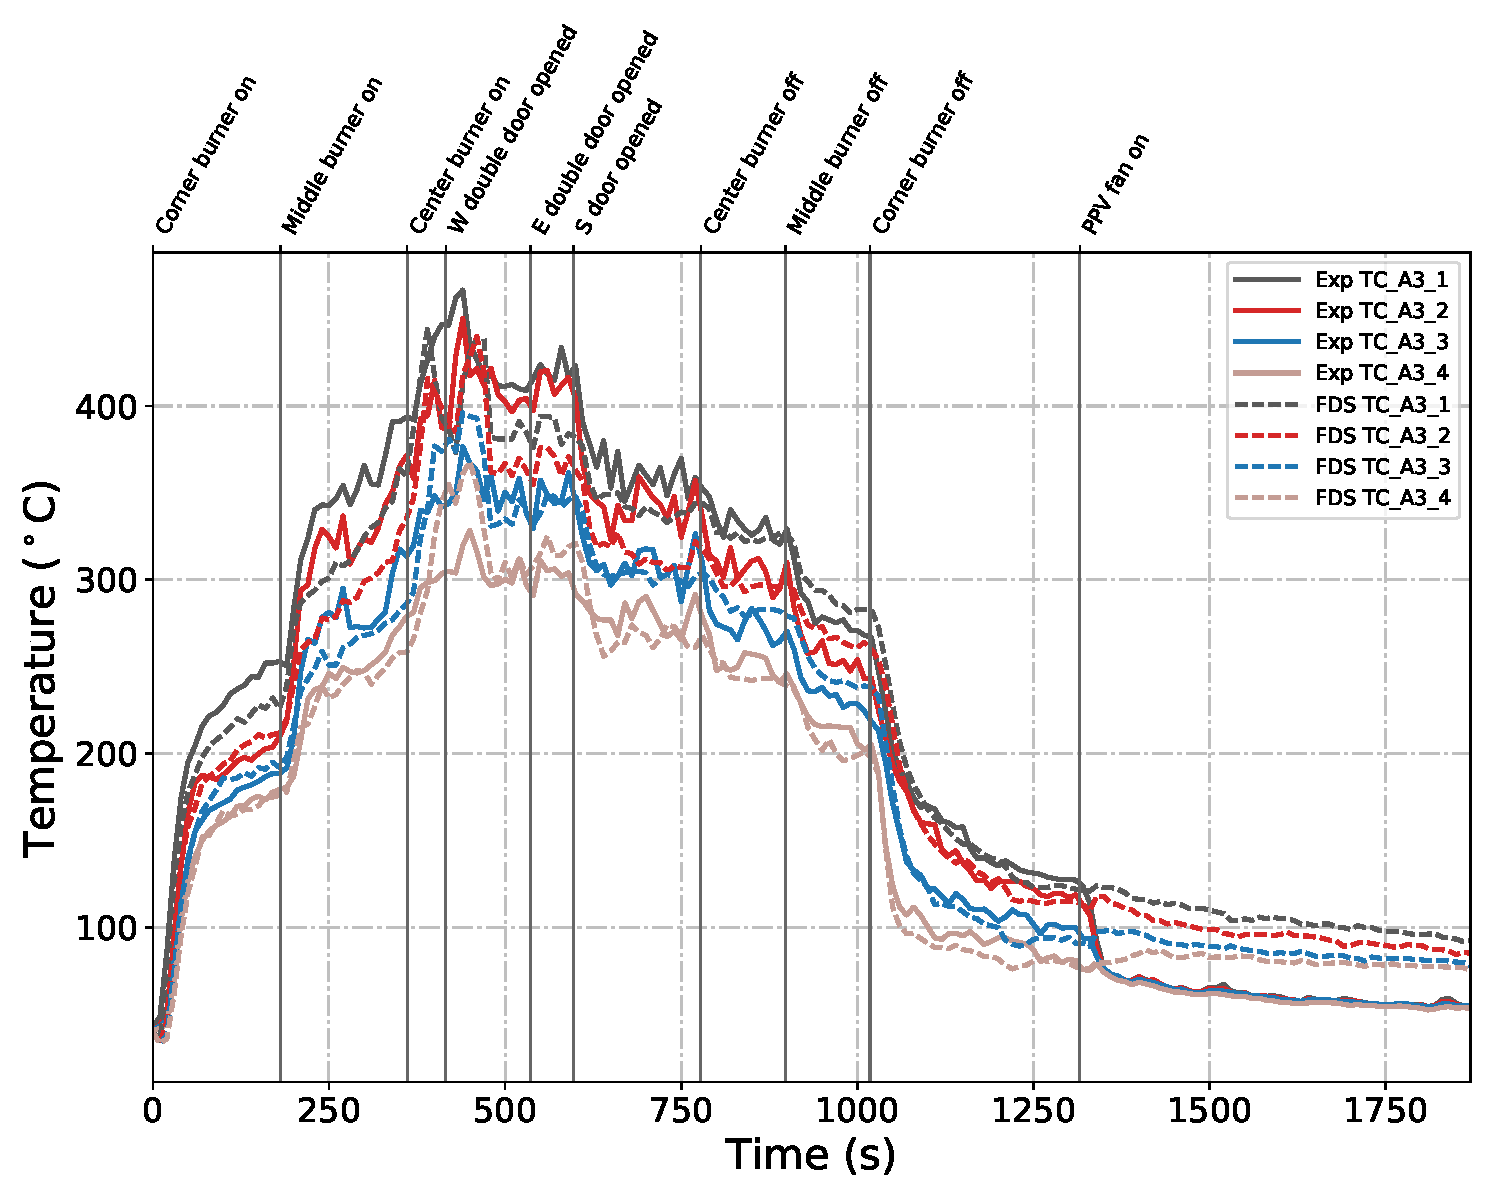
\includegraphics[width=\columnwidth]{Figures/Plots/Validation/Temperature/Test_3_TC_A3_upper}
% 	\caption{Plots of measured and predicted ``upper'' temperatures at array A3 during Test~3 in the East Structure.}
% 	\label{fig:TCA3_upper_data_Test3}
% \end{figure}

% \begin{figure}[!h]
% 	\centering
% 	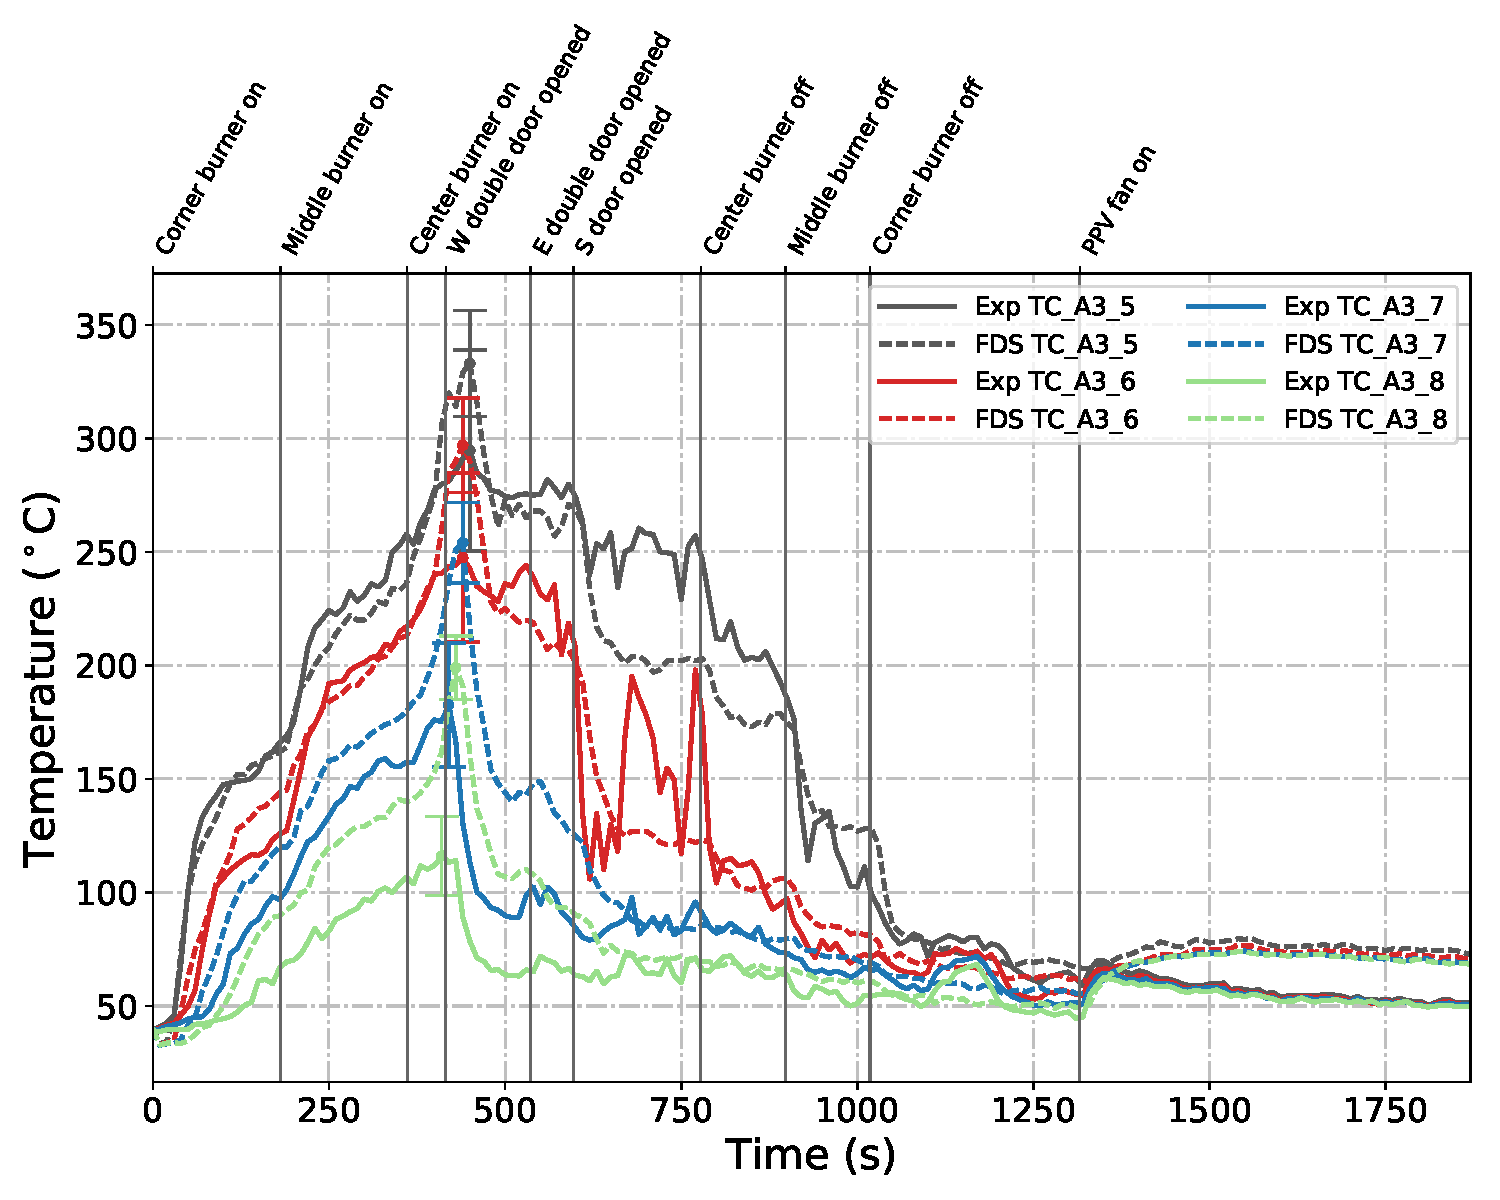
\includegraphics[width=\columnwidth]{Figures/Plots/Validation/Temperature/Test_3_TC_A3_lower}
% 	\caption{Plots of measured and predicted ``lower'' temperatures at array A3 during Test~3 in the East Structure.}
% 	\label{fig:TCA3_lower_data_Test3}
% \end{figure}

% \begin{figure}[!h]
% 	\centering
% 	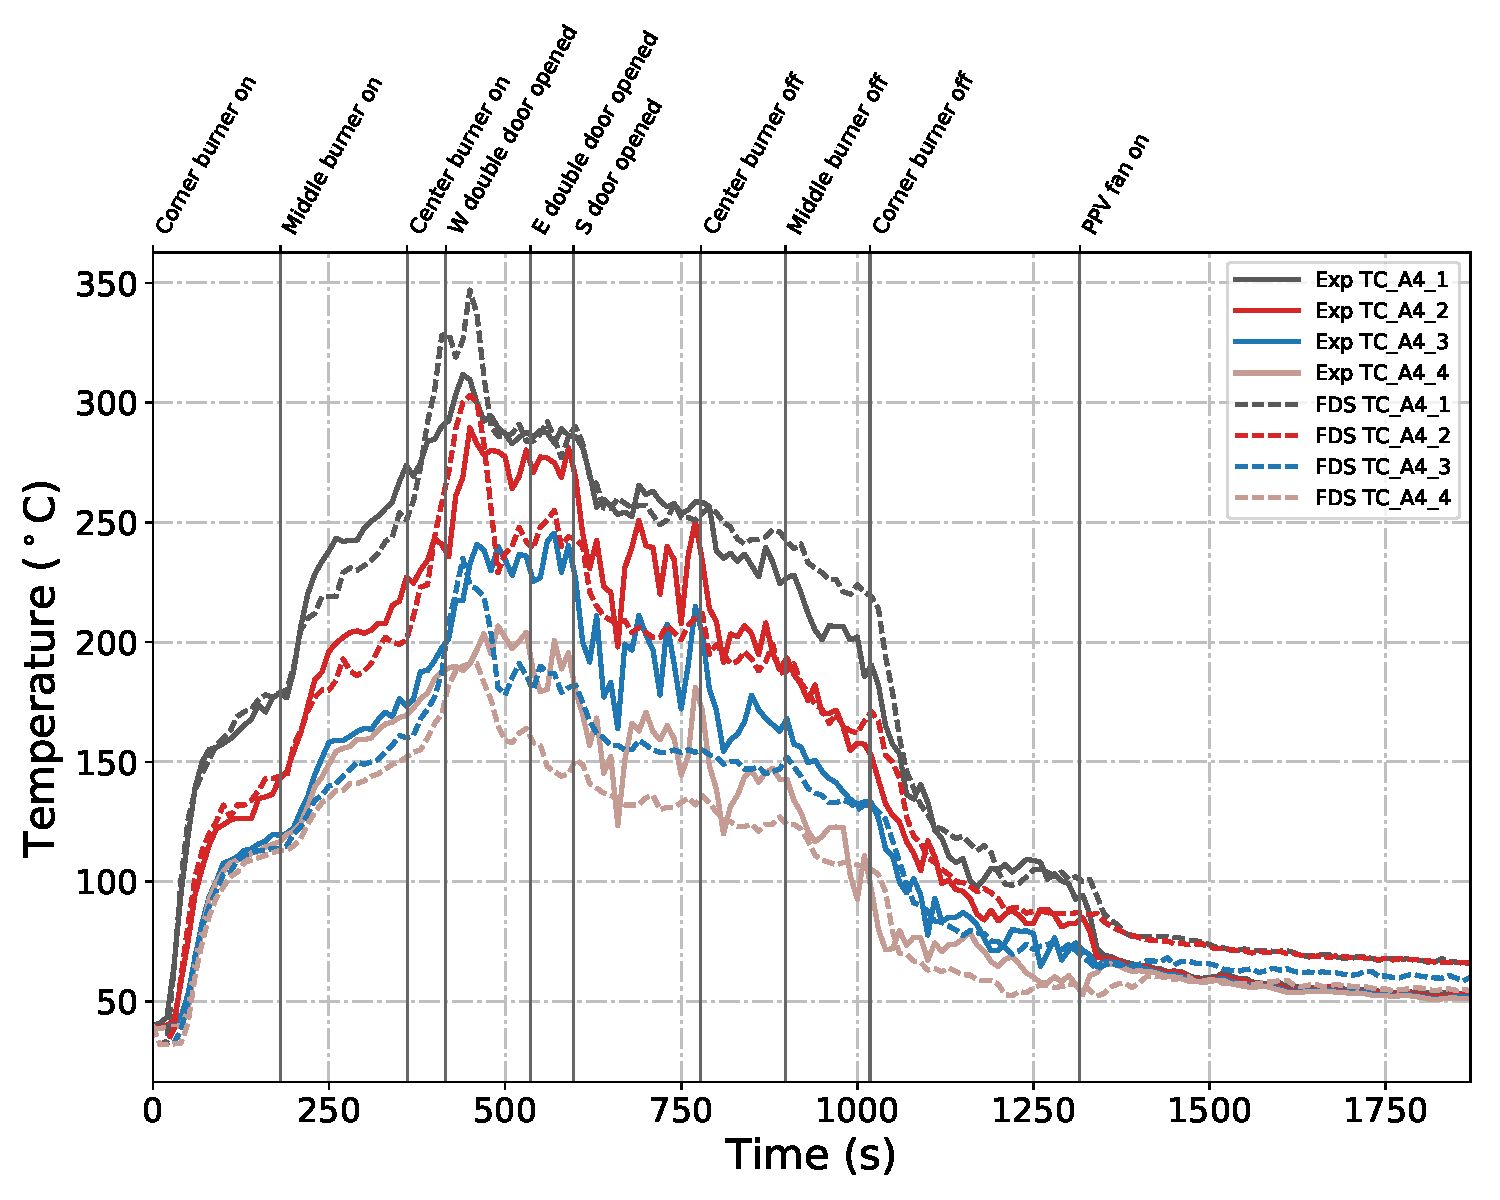
\includegraphics[width=\columnwidth]{Figures/Plots/Validation/Temperature/Test_3_TC_A4_upper}
% 	\caption{Plots of measured and predicted ``upper'' temperatures at array A4 during Test~3 in the East Structure.}
% 	\label{fig:TCA4_upper_data_Test3}
% \end{figure}

% \begin{figure}[!h]
% 	\centering
% 	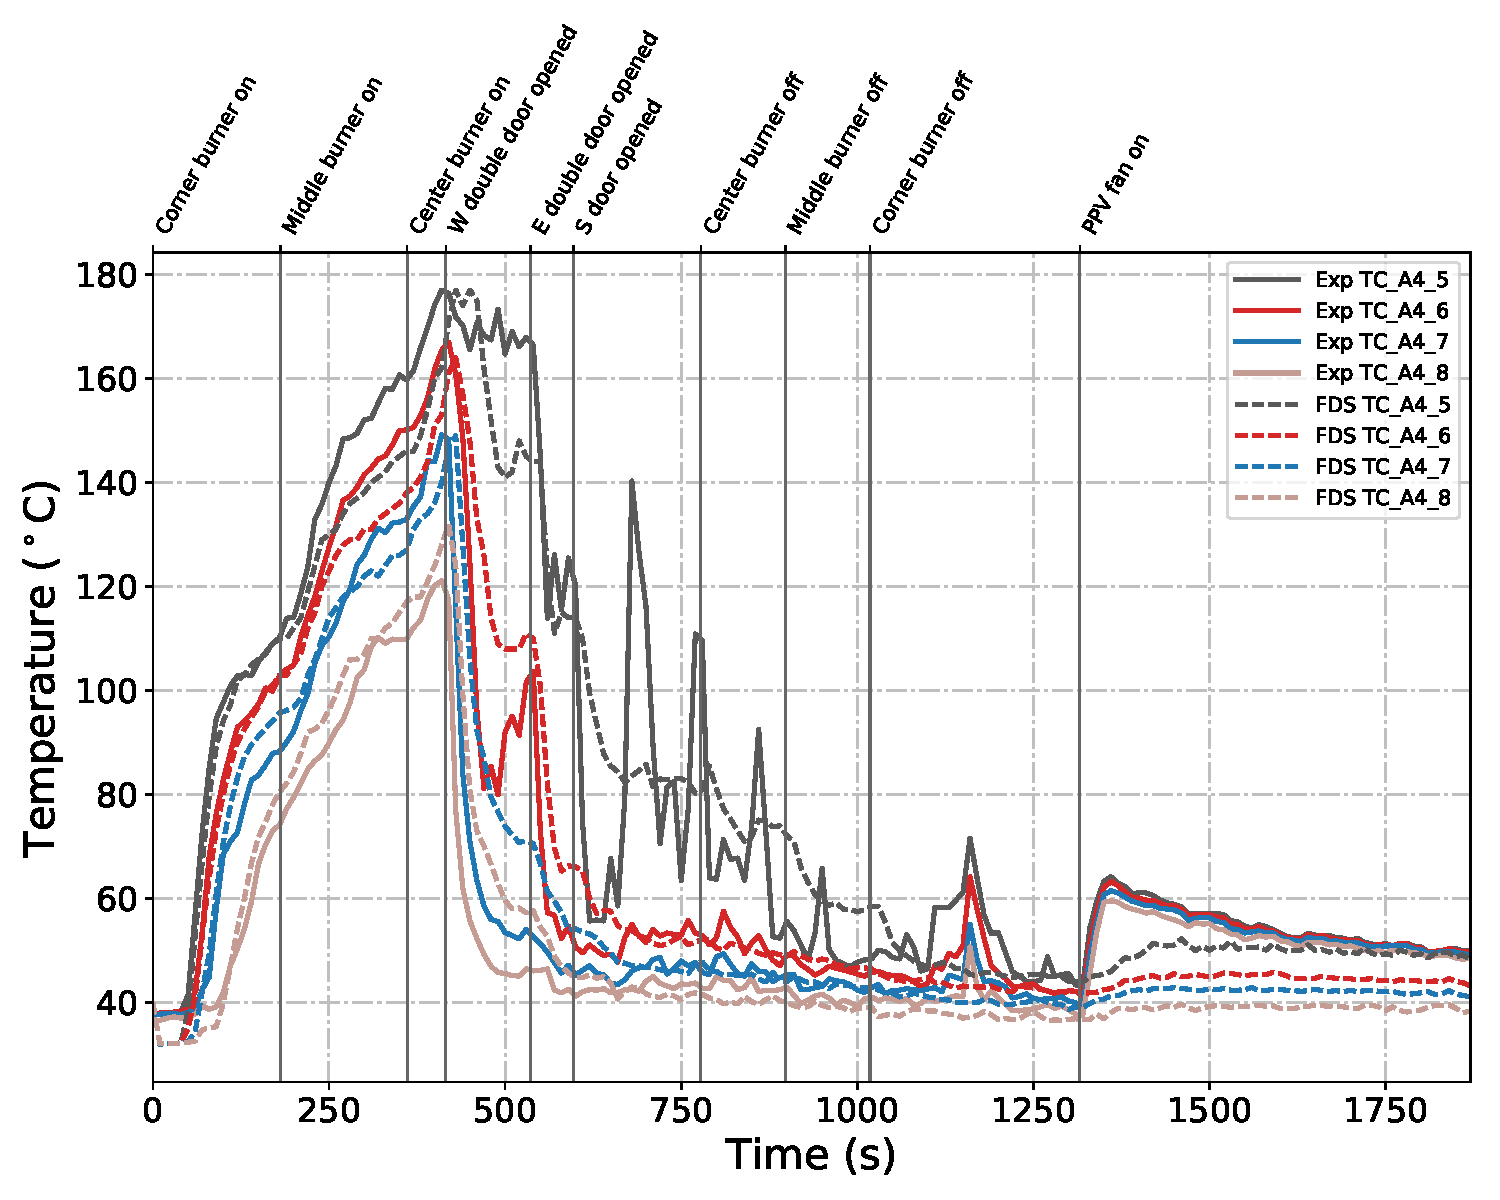
\includegraphics[width=\columnwidth]{Figures/Plots/Validation/Temperature/Test_3_TC_A4_lower}
% 	\caption{Plots of measured and predicted ``lower'' temperatures at array A4 during Test~3 in the East Structure.}
% 	\label{fig:TCA4_lower_data_Test3}
% \end{figure}

% \begin{figure}[!h]
% 	\centering
% 	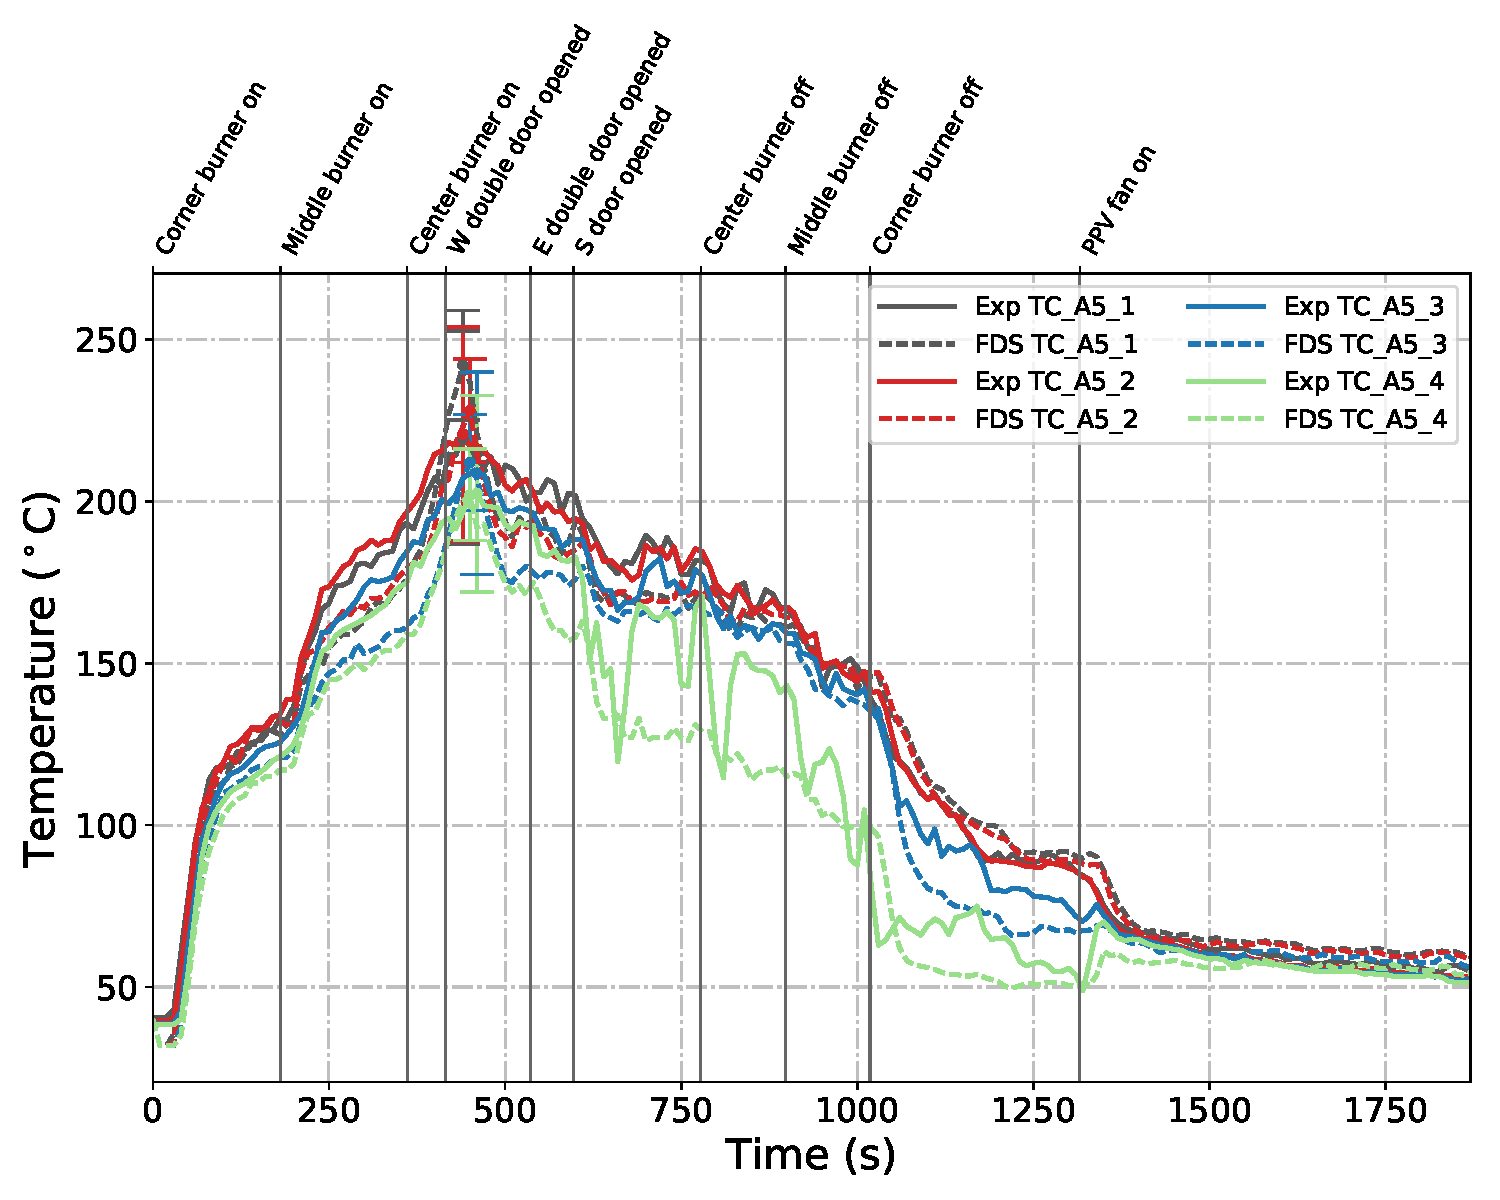
\includegraphics[width=\columnwidth]{Figures/Plots/Validation/Temperature/Test_3_TC_A5_upper}
% 	\caption{Plots of measured and predicted ``upper'' temperatures at array A5 during Test~3 in the East Structure.}
% 	\label{fig:TCA5_upper_data_Test3}
% \end{figure}

% \begin{figure}[!h]
% 	\centering
% 	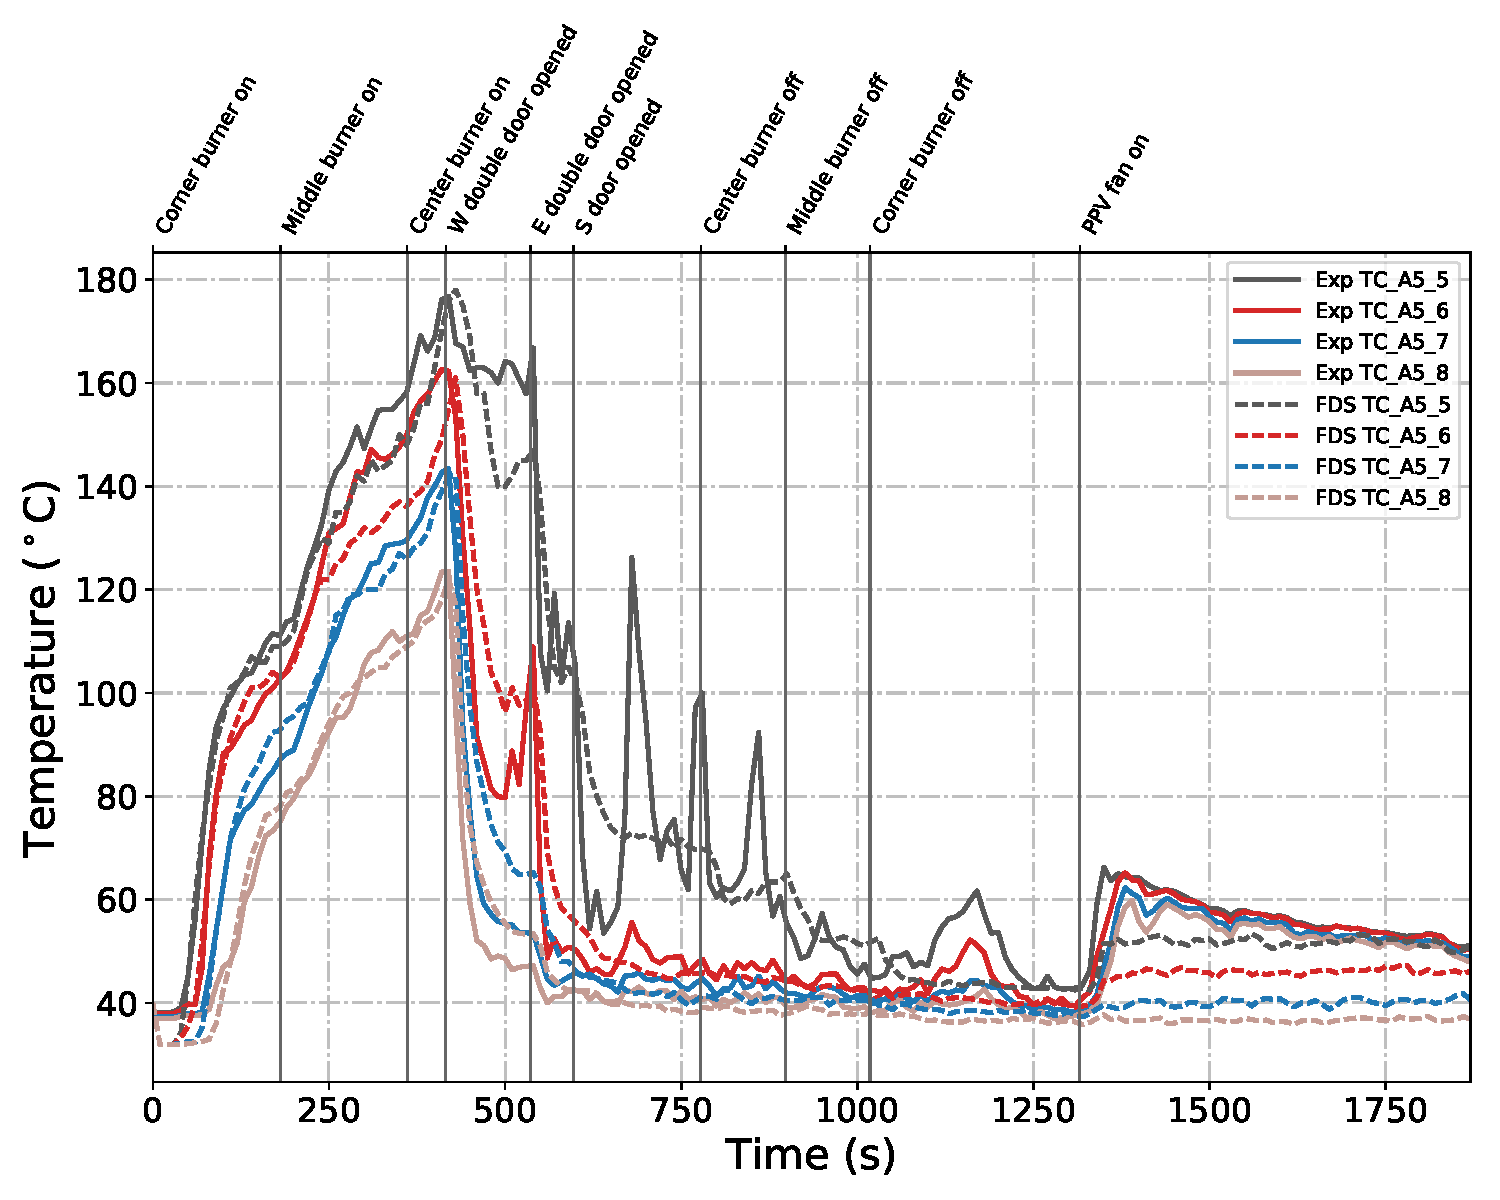
\includegraphics[width=\columnwidth]{Figures/Plots/Validation/Temperature/Test_3_TC_A5_lower}
% 	\caption{Plots of measured and predicted ``lower'' temperatures at array A5 during Test~3 in the East Structure.}
% 	\label{fig:TCA5_lower_data_Test3}
% \end{figure}

% %%%%%%%%%%%%%%%%%%%%%%%%%%%%%%%%%%%%%%%%
% \begin{figure}[!h]
% 	\centering
% 	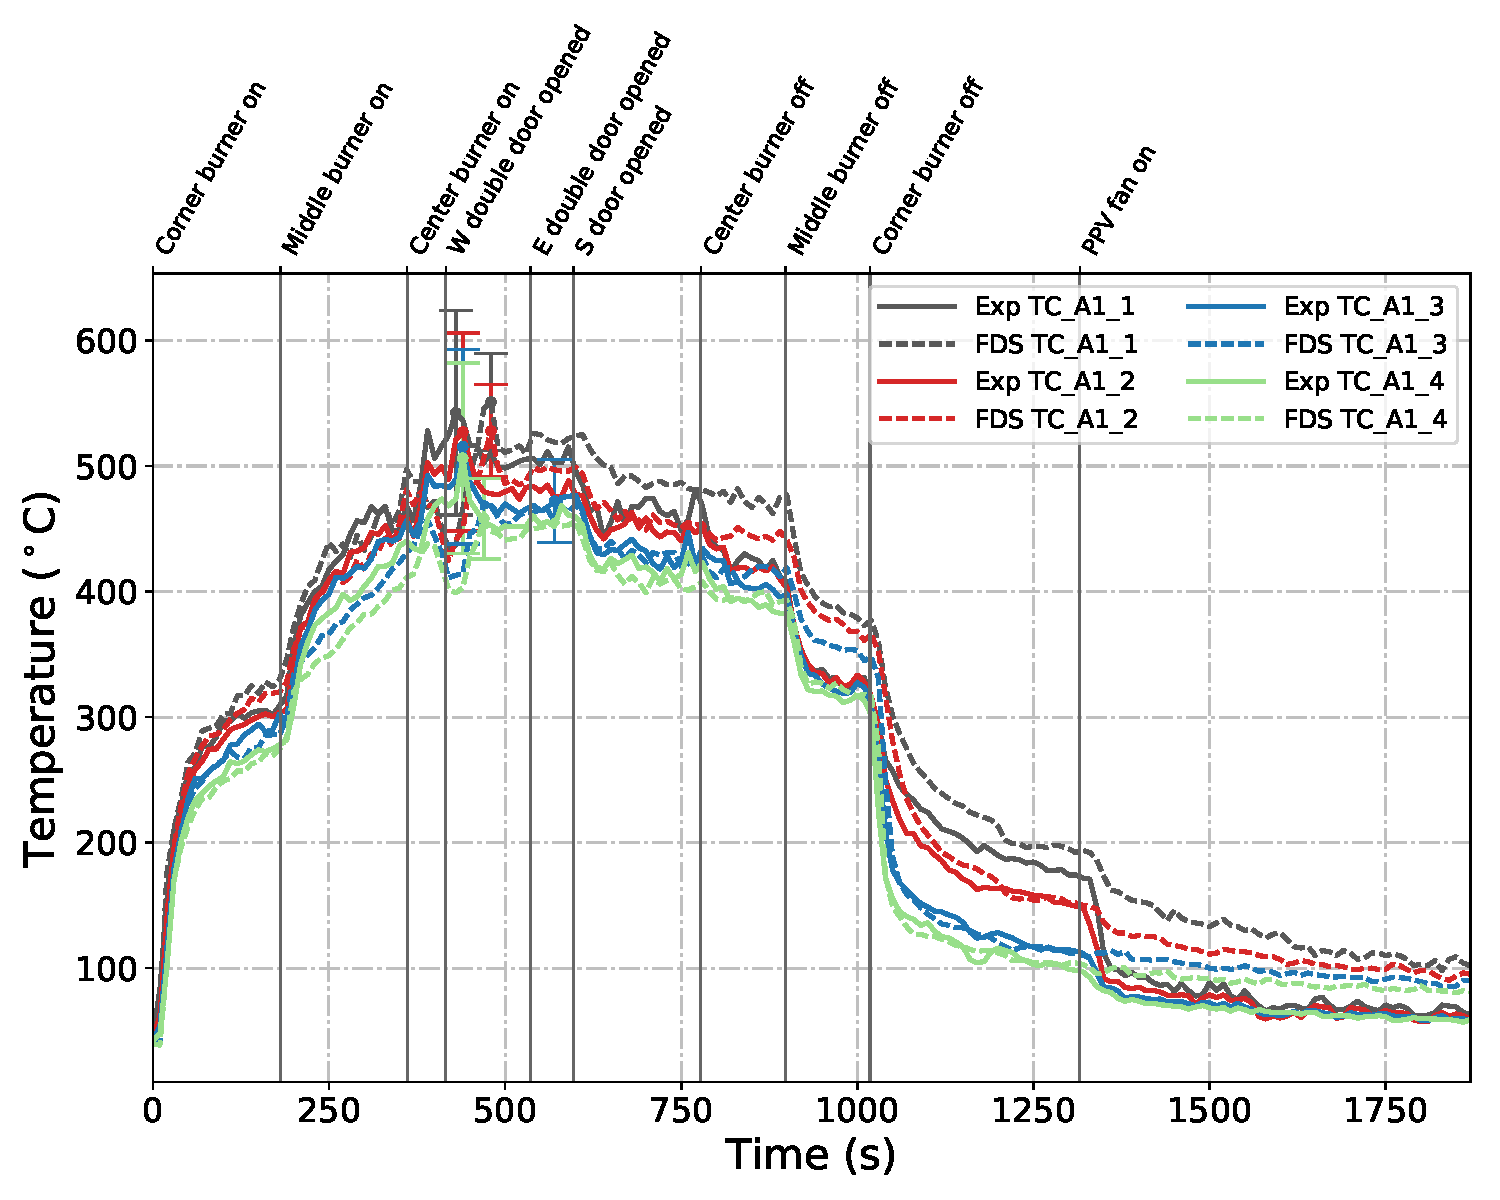
\includegraphics[width=\columnwidth]{Figures/Plots/Validation/Temperature/Test_3_TC_A1_upper}
% 	\caption{Plots of measured and predicted ``upper'' temperatures at array A1 during Test~3 in the East Structure.}
% 	\label{fig:TCA1_upper_data_Test3}
% \end{figure}

% \begin{figure}[!h]
% 	\centering
% 	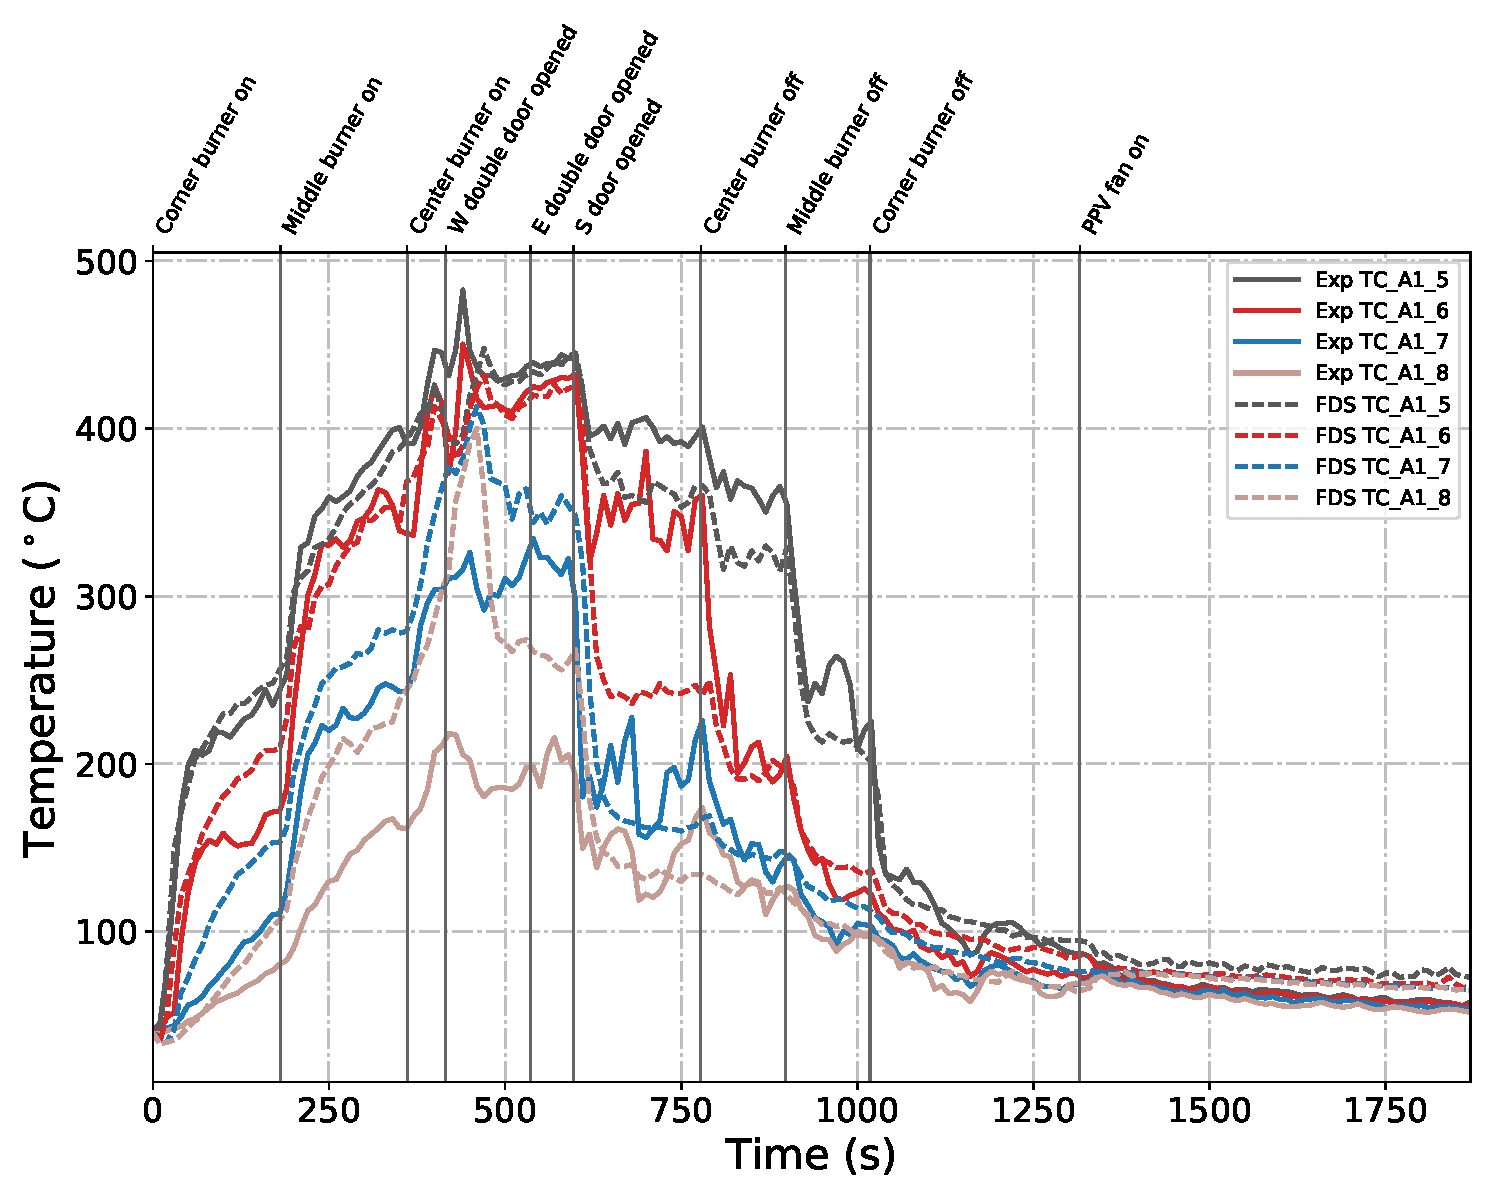
\includegraphics[width=\columnwidth]{Figures/Plots/Validation/Temperature/Test_3_TC_A1_lower}
% 	\caption{Plots of measured and predicted ``lower'' temperatures at array A1 during Test~3 in the East Structure.}
% 	\label{fig:TCA1_lower_data_Test3}
% \end{figure}

% \begin{figure}[!h]
% 	\centering
% 	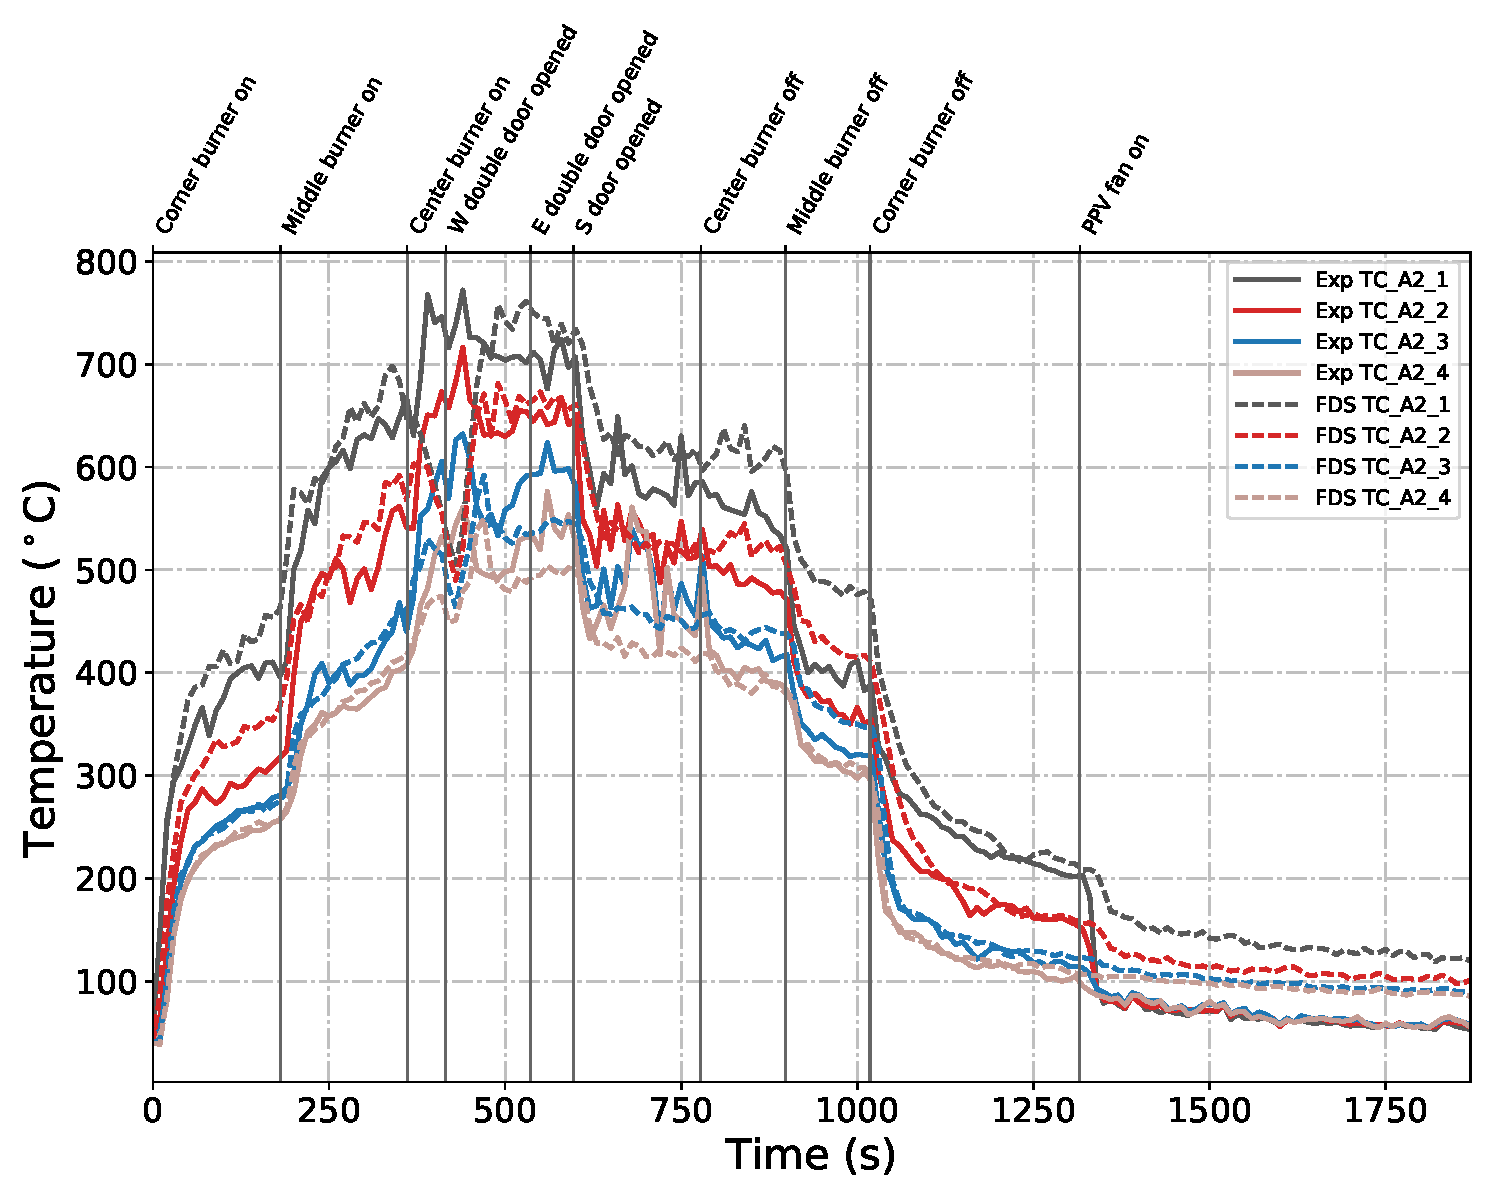
\includegraphics[width=\columnwidth]{Figures/Plots/Validation/Temperature/Test_3_TC_A2_upper}
% 	\caption{Plots of measured and predicted ``upper'' temperatures at array A2 during Test~3 in the East Structure.}
% 	\label{fig:TCA2_upper_data_Test3}
% \end{figure}

% \begin{figure}[!h]
% 	\centering
% 	\includegraphics[width=\columnwidth]{Figures/Plots/Validation/Temperature/Test_3_TC_A2_lower}
% 	\caption{Plots of measured and predicted ``lower'' temperatures at array A2 during Test~3 in the East Structure.}
% 	\label{fig:TCA2_lower_data_Test3}
% \end{figure}

% \begin{figure}[!h]
% 	\centering
% 	\includegraphics[width=\columnwidth]{Figures/Plots/Validation/Temperature/Test_3_TC_A3_upper}
% 	\caption{Plots of measured and predicted ``upper'' temperatures at array A3 during Test~3 in the East Structure.}
% 	\label{fig:TCA3_upper_data_Test3}
% \end{figure}

% \begin{figure}[!h]
% 	\centering
% 	\includegraphics[width=\columnwidth]{Figures/Plots/Validation/Temperature/Test_3_TC_A3_lower}
% 	\caption{Plots of measured and predicted ``lower'' temperatures at array A3 during Test~3 in the East Structure.}
% 	\label{fig:TCA3_lower_data_Test3}
% \end{figure}

% \begin{figure}[!h]
% 	\centering
% 	\includegraphics[width=\columnwidth]{Figures/Plots/Validation/Temperature/Test_3_TC_A4_upper}
% 	\caption{Plots of measured and predicted ``upper'' temperatures at array A4 during Test~3 in the East Structure.}
% 	\label{fig:TCA4_upper_data_Test3}
% \end{figure}

% \begin{figure}[!h]
% 	\centering
% 	\includegraphics[width=\columnwidth]{Figures/Plots/Validation/Temperature/Test_3_TC_A4_lower}
% 	\caption{Plots of measured and predicted ``lower'' temperatures at array A4 during Test~3 in the East Structure.}
% 	\label{fig:TCA4_lower_data_Test3}
% \end{figure}

% \begin{figure}[!h]
% 	\centering
% 	\includegraphics[width=\columnwidth]{Figures/Plots/Validation/Temperature/Test_3_TC_A5_upper}
% 	\caption{Plots of measured and predicted ``upper'' temperatures at array A5 during Test~3 in the East Structure.}
% 	\label{fig:TCA5_upper_data_Test3}
% \end{figure}

% \begin{figure}[!h]
% 	\centering
% 	\includegraphics[width=\columnwidth]{Figures/Plots/Validation/Temperature/Test_3_TC_A5_lower}
% 	\caption{Plots of measured and predicted ``lower'' temperatures at array A5 during Test~3 in the East Structure.}
% 	\label{fig:TCA5_lower_data_Test3}
% \end{figure}

% %%%%%%%%%%%%%%%%%%%%%%%%%%%%%%%%%%%%%%%%
% \begin{figure}[!h]
% 	\centering
% 	\includegraphics[width=\columnwidth]{Figures/Plots/Validation/Temperature/Test_5_TC_A1_upper}
% 	\caption{Plots of measured and predicted ``upper'' temperatures at array A1 during Test~5 in the East Structure.}
% 	\label{fig:TCA1_upper_data_Test5}
% \end{figure}

% \begin{figure}[!h]
% 	\centering
% 	\includegraphics[width=\columnwidth]{Figures/Plots/Validation/Temperature/Test_5_TC_A1_lower}
% 	\caption{Plots of measured and predicted ``lower'' temperatures at array A1 during Test~5 in the East Structure.}
% 	\label{fig:TCA1_lower_data_Test5}
% \end{figure}

% \begin{figure}[!h]
% 	\centering
% 	\includegraphics[width=\columnwidth]{Figures/Plots/Validation/Temperature/Test_5_TC_A2_upper}
% 	\caption{Plots of measured and predicted ``upper'' temperatures at array A2 during Test~5 in the East Structure.}
% 	\label{fig:TCA2_upper_data_Test5}
% \end{figure}

% \begin{figure}[!h]
% 	\centering
% 	\includegraphics[width=\columnwidth]{Figures/Plots/Validation/Temperature/Test_5_TC_A2_lower}
% 	\caption{Plots of measured and predicted ``lower'' temperatures at array A2 during Test~5 in the East Structure.}
% 	\label{fig:TCA2_lower_data_Test5}
% \end{figure}

% \begin{figure}[!h]
% 	\centering
% 	\includegraphics[width=\columnwidth]{Figures/Plots/Validation/Temperature/Test_5_TC_A3_upper}
% 	\caption{Plots of measured and predicted ``upper'' temperatures at array A3 during Test~5 in the East Structure.}
% 	\label{fig:TCA3_upper_data_Test5}
% \end{figure}

% \begin{figure}[!h]
% 	\centering
% 	\includegraphics[width=\columnwidth]{Figures/Plots/Validation/Temperature/Test_5_TC_A3_lower}
% 	\caption{Plots of measured and predicted ``lower'' temperatures at array A3 during Test~5 in the East Structure.}
% 	\label{fig:TCA3_lower_data_Test5}
% \end{figure}

% \begin{figure}[!h]
% 	\centering
% 	\includegraphics[width=\columnwidth]{Figures/Plots/Validation/Temperature/Test_5_TC_A4_upper}
% 	\caption{Plots of measured and predicted ``upper'' temperatures at array A4 during Test~5 in the East Structure.}
% 	\label{fig:TCA4_upper_data_Test5}
% \end{figure}

% \begin{figure}[!h]
% 	\centering
% 	\includegraphics[width=\columnwidth]{Figures/Plots/Validation/Temperature/Test_5_TC_A4_lower}
% 	\caption{Plots of measured and predicted ``lower'' temperatures at array A4 during Test~5 in the East Structure.}
% 	\label{fig:TCA4_lower_data_Test5}
% \end{figure}

% \begin{figure}[!h]
% 	\centering
% 	\includegraphics[width=\columnwidth]{Figures/Plots/Validation/Temperature/Test_5_TC_A5_upper}
% 	\caption{Plots of measured and predicted ``upper'' temperatures at array A5 during Test~5 in the East Structure.}
% 	\label{fig:TCA5_upper_data_Test5}
% \end{figure}

% \begin{figure}[!h]
% 	\centering
% 	\includegraphics[width=\columnwidth]{Figures/Plots/Validation/Temperature/Test_5_TC_A5_lower}
% 	\caption{Plots of measured and predicted ``lower'' temperatures at array A5 during Test~5 in the East Structure.}
% 	\label{fig:TCA5_lower_data_Test5}
% \end{figure}

% %%%%%%%%%%%%%%%%%%%%%%%%%%%%%%%%%%%%%%%%
% \begin{figure}[!h]
% 	\centering
% 	\includegraphics[width=\columnwidth]{Figures/Plots/Validation/Temperature/Test_3_TC_A1_upper}
% 	\caption{Plots of measured and predicted ``upper'' temperatures at array A1 during Test~3 in the East Structure.}
% 	\label{fig:TCA1_upper_data_Test3}
% \end{figure}

% \begin{figure}[!h]
% 	\centering
% 	\includegraphics[width=\columnwidth]{Figures/Plots/Validation/Temperature/Test_3_TC_A1_lower}
% 	\caption{Plots of measured and predicted ``lower'' temperatures at array A1 during Test~3 in the East Structure.}
% 	\label{fig:TCA1_lower_data_Test3}
% \end{figure}

% \begin{figure}[!h]
% 	\centering
% 	\includegraphics[width=\columnwidth]{Figures/Plots/Validation/Temperature/Test_3_TC_A2_upper}
% 	\caption{Plots of measured and predicted ``upper'' temperatures at array A2 during Test~3 in the East Structure.}
% 	\label{fig:TCA2_upper_data_Test3}
% \end{figure}

% \begin{figure}[!h]
% 	\centering
% 	\includegraphics[width=\columnwidth]{Figures/Plots/Validation/Temperature/Test_3_TC_A2_lower}
% 	\caption{Plots of measured and predicted ``lower'' temperatures at array A2 during Test~3 in the East Structure.}
% 	\label{fig:TCA2_lower_data_Test3}
% \end{figure}

% \begin{figure}[!h]
% 	\centering
% 	\includegraphics[width=\columnwidth]{Figures/Plots/Validation/Temperature/Test_3_TC_A3_upper}
% 	\caption{Plots of measured and predicted ``upper'' temperatures at array A3 during Test~3 in the East Structure.}
% 	\label{fig:TCA3_upper_data_Test3}
% \end{figure}

% \begin{figure}[!h]
% 	\centering
% 	\includegraphics[width=\columnwidth]{Figures/Plots/Validation/Temperature/Test_3_TC_A3_lower}
% 	\caption{Plots of measured and predicted ``lower'' temperatures at array A3 during Test~3 in the East Structure.}
% 	\label{fig:TCA3_lower_data_Test3}
% \end{figure}

% \begin{figure}[!h]
% 	\centering
% 	\includegraphics[width=\columnwidth]{Figures/Plots/Validation/Temperature/Test_3_TC_A4_upper}
% 	\caption{Plots of measured and predicted ``upper'' temperatures at array A4 during Test~3 in the East Structure.}
% 	\label{fig:TCA4_upper_data_Test3}
% \end{figure}

% \begin{figure}[!h]
% 	\centering
% 	\includegraphics[width=\columnwidth]{Figures/Plots/Validation/Temperature/Test_3_TC_A4_lower}
% 	\caption{Plots of measured and predicted ``lower'' temperatures at array A4 during Test~3 in the East Structure.}
% 	\label{fig:TCA4_lower_data_Test3}
% \end{figure}

% \begin{figure}[!h]
% 	\centering
% 	\includegraphics[width=\columnwidth]{Figures/Plots/Validation/Temperature/Test_3_TC_A5_upper}
% 	\caption{Plots of measured and predicted ``upper'' temperatures at array A5 during Test~3 in the East Structure.}
% 	\label{fig:TCA5_upper_data_Test3}
% \end{figure}

% \begin{figure}[!h]
% 	\centering
% 	\includegraphics[width=\columnwidth]{Figures/Plots/Validation/Temperature/Test_3_TC_A5_lower}
% 	\caption{Plots of measured and predicted ``lower'' temperatures at array A5 during Test~3 in the East Structure.}
% 	\label{fig:TCA5_lower_data_Test3}
% \end{figure}

% %%%%%%%%%%%%%%%%%%%%%%%%%%%%%%%%%%%%%%%%
% \begin{figure}[!h]
% 	\centering
% 	\includegraphics[width=\columnwidth]{Figures/Plots/Validation/Temperature/Test_6_TC_A1_upper}
% 	\caption{Plots of measured and predicted ``upper'' temperatures at array A1 during Test~6 in the East Structure.}
% 	\label{fig:TCA1_upper_data_Test6}
% \end{figure}

% \begin{figure}[!h]
% 	\centering
% 	\includegraphics[width=\columnwidth]{Figures/Plots/Validation/Temperature/Test_6_TC_A1_lower}
% 	\caption{Plots of measured and predicted ``lower'' temperatures at array A1 during Test~6 in the East Structure.}
% 	\label{fig:TCA1_lower_data_Test6}
% \end{figure}

% \begin{figure}[!h]
% 	\centering
% 	\includegraphics[width=\columnwidth]{Figures/Plots/Validation/Temperature/Test_6_TC_A2_upper}
% 	\caption{Plots of measured and predicted ``upper'' temperatures at array A2 during Test~6 in the East Structure.}
% 	\label{fig:TCA2_upper_data_Test6}
% \end{figure}

% \begin{figure}[!h]
% 	\centering
% 	\includegraphics[width=\columnwidth]{Figures/Plots/Validation/Temperature/Test_6_TC_A2_lower}
% 	\caption{Plots of measured and predicted ``lower'' temperatures at array A2 during Test~6 in the East Structure.}
% 	\label{fig:TCA2_lower_data_Test6}
% \end{figure}

% \begin{figure}[!h]
% 	\centering
% 	\includegraphics[width=\columnwidth]{Figures/Plots/Validation/Temperature/Test_6_TC_A3_upper}
% 	\caption{Plots of measured and predicted ``upper'' temperatures at array A3 during Test~6 in the East Structure.}
% 	\label{fig:TCA3_upper_data_Test6}
% \end{figure}

% \begin{figure}[!h]
% 	\centering
% 	\includegraphics[width=\columnwidth]{Figures/Plots/Validation/Temperature/Test_6_TC_A3_lower}
% 	\caption{Plots of measured and predicted ``lower'' temperatures at array A3 during Test~6 in the East Structure.}
% 	\label{fig:TCA3_lower_data_Test6}
% \end{figure}

% \begin{figure}[!h]
% 	\centering
% 	\includegraphics[width=\columnwidth]{Figures/Plots/Validation/Temperature/Test_6_TC_A4_upper}
% 	\caption{Plots of measured and predicted ``upper'' temperatures at array A4 during Test~6 in the East Structure.}
% 	\label{fig:TCA4_upper_data_Test6}
% \end{figure}

% \begin{figure}[!h]
% 	\centering
% 	\includegraphics[width=\columnwidth]{Figures/Plots/Validation/Temperature/Test_6_TC_A4_lower}
% 	\caption{Plots of measured and predicted ``lower'' temperatures at array A4 during Test~6 in the East Structure.}
% 	\label{fig:TCA4_lower_data_Test6}
% \end{figure}

% \begin{figure}[!h]
% 	\centering
% 	\includegraphics[width=\columnwidth]{Figures/Plots/Validation/Temperature/Test_6_TC_A5_upper}
% 	\caption{Plots of measured and predicted ``upper'' temperatures at array A5 during Test~6 in the East Structure.}
% 	\label{fig:TCA5_upper_data_Test6}
% \end{figure}

% \begin{figure}[!h]
% 	\centering
% 	\includegraphics[width=\columnwidth]{Figures/Plots/Validation/Temperature/Test_6_TC_A5_lower}
% 	\caption{Plots of measured and predicted ``lower'' temperatures at array A5 during Test~6 in the East Structure.}
% 	\label{fig:TCA5_lower_data_Test6}
% \end{figure}

%%%%%%%%%%%%%%%%%%%%%%%%%%%%%%%%%%%%%%%%
%%%%%%%%%% WEST STRUCTURE %%%%%%%%%%%%%%
%%%%%%%%%%%%%%%%%%%%%%%%%%%%%%%%%%%%%%%%
\begin{figure}[!h]
	\centering
	\includegraphics[width=\columnwidth]{Figures/Plots/Validation/Temperature/Test_22_TC_A1_upper}
	\caption{Plots of measured and predicted ``upper'' temperatures at array A1 during Test~22 in the West Structure.}
	\label{fig:TCA1_upper_data_Test22}
\end{figure}

\begin{figure}[!h]
	\centering
	\includegraphics[width=\columnwidth]{Figures/Plots/Validation/Temperature/Test_22_TC_A1_lower}
	\caption{Plots of measured and predicted ``lower'' temperatures at array A1 during Test~22 in the West Structure.}
	\label{fig:TCA1_lower_data_Test22}
\end{figure}

\begin{figure}[!h]
	\centering
	\includegraphics[width=\columnwidth]{Figures/Plots/Validation/Temperature/Test_22_TC_A2_upper}
	\caption{Plots of measured and predicted ``upper'' temperatures at array A2 during Test~22 in the West Structure.}
	\label{fig:TCA2_upper_data_Test22}
\end{figure}

\begin{figure}[!h]
	\centering
	\includegraphics[width=\columnwidth]{Figures/Plots/Validation/Temperature/Test_22_TC_A2_lower}
	\caption{Plots of measured and predicted ``lower'' temperatures at array A2 during Test~22 in the West Structure.}
	\label{fig:TCA2_lower_data_Test22}
\end{figure}

\begin{figure}[!h]
	\centering
	\includegraphics[width=\columnwidth]{Figures/Plots/Validation/Temperature/Test_22_TC_A3_upper}
	\caption{Plots of measured and predicted ``upper'' temperatures at array A3 during Test~22 in the West Structure.}
	\label{fig:TCA3_upper_data_Test22}
\end{figure}

\begin{figure}[!h]
	\centering
	\includegraphics[width=\columnwidth]{Figures/Plots/Validation/Temperature/Test_22_TC_A3_lower}
	\caption{Plots of measured and predicted ``lower'' temperatures at array A3 during Test~22 in the West Structure.}
	\label{fig:TCA3_lower_data_Test22}
\end{figure}

\begin{figure}[!h]
	\centering
	\includegraphics[width=\columnwidth]{Figures/Plots/Validation/Temperature/Test_22_TC_A7_upper}
	\caption{Plots of measured and predicted ``upper'' temperatures at array A7 during Test~22 in the West Structure.}
	\label{fig:TCA7_upper_data_Test22}
\end{figure}

\begin{figure}[!h]
	\centering
	\includegraphics[width=\columnwidth]{Figures/Plots/Validation/Temperature/Test_22_TC_A7_lower}
	\caption{Plots of measured and predicted ``lower'' temperatures at array A7 during Test~22 in the West Structure.}
	\label{fig:TCA7_lower_data_Test22}
\end{figure}

\begin{figure}[!h]
	\centering
	\includegraphics[width=\columnwidth]{Figures/Plots/Validation/Temperature/Test_22_TC_A8_upper}
	\caption{Plots of measured and predicted ``upper'' temperatures at array A8 during Test~22 in the West Structure.}
	\label{fig:TCA8_upper_data_Test22}
\end{figure}

\begin{figure}[!h]
	\centering
	\includegraphics[width=\columnwidth]{Figures/Plots/Validation/Temperature/Test_22_TC_A8_lower}
	\caption{Plots of measured and predicted ``lower'' temperatures at array A8 during Test~22 in the West Structure.}
	\label{fig:TCA8_lower_data_Test22}
\end{figure}

\begin{figure}[!h]
	\centering
	\includegraphics[width=\columnwidth]{Figures/Plots/Validation/Temperature/Test_22_TC_A9_upper}
	\caption{Plots of measured and predicted ``upper'' temperatures at array A9 during Test~22 in the West Structure.}
	\label{fig:TCA9_upper_data_Test22}
\end{figure}

\begin{figure}[!h]
	\centering
	\includegraphics[width=\columnwidth]{Figures/Plots/Validation/Temperature/Test_22_TC_A9_lower}
	\caption{Plots of measured and predicted ``lower'' temperatures at array A9 during Test~22 in the West Structure.}
	\label{fig:TCA9_lower_data_Test22}
\end{figure}

%%%%%%%%%%%%%%%%%%%%%%%%%%%%%%%%%%%%%%%%%%%
\begin{figure}[!h]
	\centering
	\includegraphics[width=\columnwidth]{Figures/Plots/Validation/Temperature/Test_23_TC_A1_upper}
	\caption{Plots of measured and predicted ``upper'' temperatures at array A1 during Test~23 in the West Structure.}
	\label{fig:TCA1_upper_data_Test23}
\end{figure}
\begin{figure}[!h]
	\centering
	\includegraphics[width=\columnwidth]{Figures/Plots/Validation/Temperature/Test_23_TC_A1_lower}
	\caption{Plots of measured and predicted ``lower'' temperatures at array A1 during Test~23 in the West Structure.}
	\label{fig:TCA1_lower_data_Test23}
\end{figure}

\begin{figure}[!h]
	\centering
	\includegraphics[width=\columnwidth]{Figures/Plots/Validation/Temperature/Test_23_TC_A2_upper}
	\caption{Plots of measured and predicted ``upper'' temperatures at array A2 during Test~23 in the West Structure.}
	\label{fig:TCA2_upper_data_Test23}
\end{figure}

\begin{figure}[!h]
	\centering
	\includegraphics[width=\columnwidth]{Figures/Plots/Validation/Temperature/Test_23_TC_A2_lower}
	\caption{Plots of measured and predicted ``lower'' temperatures at array A2 during Test~23 in the West Structure.}
	\label{fig:TCA2_lower_data_Test23}
\end{figure}

\begin{figure}[!h]
	\centering
	\includegraphics[width=\columnwidth]{Figures/Plots/Validation/Temperature/Test_23_TC_A3_upper}
	\caption{Plots of measured and predicted ``upper'' temperatures at array A3 during Test~23 in the West Structure.}
	\label{fig:TCA3_upper_data_Test23}
\end{figure}

\begin{figure}[!h]
	\centering
	\includegraphics[width=\columnwidth]{Figures/Plots/Validation/Temperature/Test_23_TC_A3_lower}
	\caption{Plots of measured and predicted ``lower'' temperatures at array A3 during Test~23 in the West Structure.}
	\label{fig:TCA3_lower_data_Test23}
\end{figure}

\begin{figure}[!h]
	\centering
	\includegraphics[width=\columnwidth]{Figures/Plots/Validation/Temperature/Test_23_TC_A7_upper}
	\caption{Plots of measured and predicted ``upper'' temperatures at array A7 during Test~23 in the West Structure.}
	\label{fig:TCA7_upper_data_Test23}
\end{figure}

\begin{figure}[!h]
	\centering
	\includegraphics[width=\columnwidth]{Figures/Plots/Validation/Temperature/Test_23_TC_A7_lower}
	\caption{Plots of measured and predicted ``lower'' temperatures at array A7 during Test~23 in the West Structure.}
	\label{fig:TCA7_lower_data_Test23}
\end{figure}

\begin{figure}[!h]
	\centering
	\includegraphics[width=\columnwidth]{Figures/Plots/Validation/Temperature/Test_23_TC_A8_upper}
	\caption{Plots of measured and predicted ``upper'' temperatures at array A8 during Test~23 in the West Structure.}
	\label{fig:TCA8_upper_data_Test23}
\end{figure}

\begin{figure}[!h]
	\centering
	\includegraphics[width=\columnwidth]{Figures/Plots/Validation/Temperature/Test_23_TC_A8_lower}
	\caption{Plots of measured and predicted ``lower'' temperatures at array A8 during Test~23 in the West Structure.}
	\label{fig:TCA8_lower_data_Test23}
\end{figure}

\begin{figure}[!h]
	\centering
	\includegraphics[width=\columnwidth]{Figures/Plots/Validation/Temperature/Test_23_TC_A9_upper}
	\caption{Plots of measured and predicted ``upper'' temperatures at array A9 during Test~23 in the West Structure.}
	\label{fig:TCA9_upper_data_Test23}
\end{figure}

\begin{figure}[!h]
	\centering
	\includegraphics[width=\columnwidth]{Figures/Plots/Validation/Temperature/Test_23_TC_A9_lower}
	\caption{Plots of measured and predicted ``lower'' temperatures at array A9 during Test~23 in the West Structure.}
	\label{fig:TCA9_lower_data_Test23}
\end{figure}
%%%%%%%%%%%%%%%%%%%%
\begin{figure}[!h]
	\centering
	\includegraphics[width=\columnwidth]{Figures/Plots/Validation/Temperature/Test_24_TC_A1_lower}
	\caption{Plots of measured and predicted ``lower'' temperatures at array A1 during Test~24 in the West Structure.}
	\label{fig:TCA1_lower_data_Test24}
\end{figure}

\begin{figure}[!h]
	\centering
	\includegraphics[width=\columnwidth]{Figures/Plots/Validation/Temperature/Test_24_TC_A2_upper}
	\caption{Plots of measured and predicted ``upper'' temperatures at array A2 during Test~24 in the West Structure.}
	\label{fig:TCA2_upper_data_Test24}
\end{figure}

\begin{figure}[!h]
	\centering
	\includegraphics[width=\columnwidth]{Figures/Plots/Validation/Temperature/Test_24_TC_A2_lower}
	\caption{Plots of measured and predicted ``lower'' temperatures at array A2 during Test~24 in the West Structure.}
	\label{fig:TCA2_lower_data_Test24}
\end{figure}

\begin{figure}[!h]
	\centering
	\includegraphics[width=\columnwidth]{Figures/Plots/Validation/Temperature/Test_24_TC_A3_upper}
	\caption{Plots of measured and predicted ``upper'' temperatures at array A3 during Test~24 in the West Structure.}
	\label{fig:TCA3_upper_data_Test24}
\end{figure}

\begin{figure}[!h]
	\centering
	\includegraphics[width=\columnwidth]{Figures/Plots/Validation/Temperature/Test_24_TC_A3_lower}
	\caption{Plots of measured and predicted ``lower'' temperatures at array A3 during Test~24 in the West Structure.}
	\label{fig:TCA3_lower_data_Test24}
\end{figure}

\begin{figure}[!h]
	\centering
	\includegraphics[width=\columnwidth]{Figures/Plots/Validation/Temperature/Test_24_TC_A7_upper}
	\caption{Plots of measured and predicted ``upper'' temperatures at array A7 during Test~24 in the West Structure.}
	\label{fig:TCA7_upper_data_Test24}
\end{figure}

\begin{figure}[!h]
	\centering
	\includegraphics[width=\columnwidth]{Figures/Plots/Validation/Temperature/Test_24_TC_A7_lower}
	\caption{Plots of measured and predicted ``lower'' temperatures at array A7 during Test~24 in the West Structure.}
	\label{fig:TCA7_lower_data_Test24}
\end{figure}

\begin{figure}[!h]
	\centering
	\includegraphics[width=\columnwidth]{Figures/Plots/Validation/Temperature/Test_24_TC_A8_upper}
	\caption{Plots of measured and predicted ``upper'' temperatures at array A8 during Test~24 in the West Structure.}
	\label{fig:TCA8_upper_data_Test24}
\end{figure}

\begin{figure}[!h]
	\centering
	\includegraphics[width=\columnwidth]{Figures/Plots/Validation/Temperature/Test_24_TC_A8_lower}
	\caption{Plots of measured and predicted ``lower'' temperatures at array A8 during Test~24 in the West Structure.}
	\label{fig:TCA8_lower_data_Test24}
\end{figure}

\begin{figure}[!h]
	\centering
	\includegraphics[width=\columnwidth]{Figures/Plots/Validation/Temperature/Test_24_TC_A9_upper}
	\caption{Plots of measured and predicted ``upper'' temperatures at array A9 during Test~24 in the West Structure.}
	\label{fig:TCA9_upper_data_Test24}
\end{figure}

\begin{figure}[!h]
	\centering
	\includegraphics[width=\columnwidth]{Figures/Plots/Validation/Temperature/Test_24_TC_A9_lower}
	\caption{Plots of measured and predicted ``lower'' temperatures at array A9 during Test~24 in the West Structure.}
	\label{fig:TCA9_lower_data_Test24}
\end{figure}
%%%%%%%%%%%%%%%%%%%%%%%%%%%%%%%%%%%%%%%%%%%
\begin{figure}[!h]
	\centering
	\includegraphics[width=\columnwidth]{Figures/Plots/Validation/Temperature/Test_25_TC_A1_upper}
	\caption{Plots of measured and predicted ``upper'' temperatures at array A1 during Test~25 in the West Structure.}
	\label{fig:TCA1_upper_data_Test25}
\end{figure}
\begin{figure}[!h]
	\centering
	\includegraphics[width=\columnwidth]{Figures/Plots/Validation/Temperature/Test_25_TC_A1_lower}
	\caption{Plots of measured and predicted ``lower'' temperatures at array A1 during Test~25 in the West Structure.}
	\label{fig:TCA1_lower_data_Test25}
\end{figure}

\begin{figure}[!h]
	\centering
	\includegraphics[width=\columnwidth]{Figures/Plots/Validation/Temperature/Test_25_TC_A2_upper}
	\caption{Plots of measured and predicted ``upper'' temperatures at array A2 during Test~25 in the West Structure.}
	\label{fig:TCA2_upper_data_Test25}
\end{figure}

\begin{figure}[!h]
	\centering
	\includegraphics[width=\columnwidth]{Figures/Plots/Validation/Temperature/Test_25_TC_A2_lower}
	\caption{Plots of measured and predicted ``lower'' temperatures at array A2 during Test~25 in the West Structure.}
	\label{fig:TCA2_lower_data_Test25}
\end{figure}

\begin{figure}[!h]
	\centering
	\includegraphics[width=\columnwidth]{Figures/Plots/Validation/Temperature/Test_25_TC_A3_upper}
	\caption{Plots of measured and predicted ``upper'' temperatures at array A3 during Test~25 in the West Structure.}
	\label{fig:TCA3_upper_data_Test25}
\end{figure}

\begin{figure}[!h]
	\centering
	\includegraphics[width=\columnwidth]{Figures/Plots/Validation/Temperature/Test_25_TC_A3_lower}
	\caption{Plots of measured and predicted ``lower'' temperatures at array A3 during Test~25 in the West Structure.}
	\label{fig:TCA3_lower_data_Test25}
\end{figure}

\begin{figure}[!h]
	\centering
	\includegraphics[width=\columnwidth]{Figures/Plots/Validation/Temperature/Test_25_TC_A7_upper}
	\caption{Plots of measured and predicted ``upper'' temperatures at array A7 during Test~25 in the West Structure.}
	\label{fig:TCA7_upper_data_Test25}
\end{figure}

\begin{figure}[!h]
	\centering
	\includegraphics[width=\columnwidth]{Figures/Plots/Validation/Temperature/Test_25_TC_A7_lower}
	\caption{Plots of measured and predicted ``lower'' temperatures at array A7 during Test~25 in the West Structure.}
	\label{fig:TCA7_lower_data_Test25}
\end{figure}

\begin{figure}[!h]
	\centering
	\includegraphics[width=\columnwidth]{Figures/Plots/Validation/Temperature/Test_25_TC_A8_upper}
	\caption{Plots of measured and predicted ``upper'' temperatures at array A8 during Test~25 in the West Structure.}
	\label{fig:TCA8_upper_data_Test25}
\end{figure}

\begin{figure}[!h]
	\centering
	\includegraphics[width=\columnwidth]{Figures/Plots/Validation/Temperature/Test_25_TC_A8_lower}
	\caption{Plots of measured and predicted ``lower'' temperatures at array A8 during Test~25 in the West Structure.}
	\label{fig:TCA8_lower_data_Test25}
\end{figure}

\begin{figure}[!h]
	\centering
	\includegraphics[width=\columnwidth]{Figures/Plots/Validation/Temperature/Test_25_TC_A9_upper}
	\caption{Plots of measured and predicted ``upper'' temperatures at array A9 during Test~25 in the West Structure.}
	\label{fig:TCA9_upper_data_Test25}
\end{figure}

\begin{figure}[!h]
	\centering
	\includegraphics[width=\columnwidth]{Figures/Plots/Validation/Temperature/Test_25_TC_A9_lower}
	\caption{Plots of measured and predicted ``lower'' temperatures at array A9 during Test~25 in the West Structure.}
	\label{fig:TCA9_lower_data_Test25}
\end{figure}

\clearpage
\section{Gas Species Concentration}
\subsection*{\textit{O$_2$ Concentration}}
\begin{figure}[!h]
	\centering
	\includegraphics[width=\columnwidth]{Figures/Plots/Validation/Gas_Concentration/Test_2_O2}
	\caption[Plots of measured and predicted $O_2$ concentration during Test~2.]{Plots of measured and predicted $O_2$ concentration in the fire room (black plots) and north room (red plots) of the East Structure during Test~2.}
	\label{fig:Test2_O2}
\end{figure}

\begin{figure}[!h]
	\centering
	\includegraphics[width=\columnwidth]{Figures/Plots/Validation/Gas_Concentration/Test_4_O2}
	\caption[Plots of measured and predicted $O_2$ concentration during Test~4.]{Plots of measured and predicted $O_2$ concentration in the fire room (black plots) and north room (red plots) of the East Structure during Test~4.}
	\label{fig:Test4_O2}
\end{figure}

\begin{figure}[!h]
	\centering
	\includegraphics[width=\columnwidth]{Figures/Plots/Validation/Gas_Concentration/Test_5_O2}
	\caption[Plots of measured and predicted $O_2$ concentration during Test~5.]{Plots of measured and predicted $O_2$ concentration in the fire room (black plots) and north room (red plots) of the East Structure during Test~5.}
	\label{fig:Test5_O2}
\end{figure}

\begin{figure}[!h]
	\centering
	\includegraphics[width=\columnwidth]{Figures/Plots/Validation/Gas_Concentration/Test_6_O2}
	\caption[Plots of measured and predicted $O_2$ concentration during Test~6.]{Plots of measured and predicted $O_2$ concentration in the fire room (black plots) and north room (red plots) of the East Structure during Test~6.}
	\label{fig:Test6_O2}
\end{figure}

\begin{figure}[!h]
	\centering
	\includegraphics[width=\columnwidth]{Figures/Plots/Validation/Gas_Concentration/Test_22_O2}
	\caption[Plots of measured and predicted $O_2$ concentration during Test~22.]{Plots of measured and predicted $O_2$ concentration on the first floor (black plots) and second floor (red plots) of the West Structure during Test~22.}
	\label{fig:Test22_O2}
\end{figure}

\begin{figure}[!h]
	\centering
	\includegraphics[width=\columnwidth]{Figures/Plots/Validation/Gas_Concentration/Test_23_O2}
	\caption[Plots of measured and predicted $O_2$ concentration during Test~23.]{Plots of measured and predicted $O_2$ concentration on the first floor (black plots) and second floor (red plots) of the West Structure during Test~23.}
	\label{fig:Test23_O2}
\end{figure}

\begin{figure}[!h]
	\centering
	\includegraphics[width=\columnwidth]{Figures/Plots/Validation/Gas_Concentration/Test_24_O2}
	\caption[Plots of measured and predicted $O_2$ concentration during Test~24.]{Plots of measured and predicted $O_2$ concentration on the first floor (black plots) and second floor (red plots) of the West Structure during Test~24.}
	\label{fig:Test24_O2}
\end{figure}

\begin{figure}[!h]
	\centering
	\includegraphics[width=\columnwidth]{Figures/Plots/Validation/Gas_Concentration/Test_25_O2}
	\caption[Plots of measured and predicted $O_2$ concentration during Test~25.]{Plots of measured and predicted $O_2$ concentration on the first floor (black plots) and second floor (red plots) of the West Structure during Test~25.}
	\label{fig:Test25_O2}
\end{figure}

\clearpage
\subsection*{\textit{CO$_2$ Concentration}}
\begin{figure}[!h]
	\centering
	\includegraphics[width=\columnwidth]{Figures/Plots/Validation/Gas_Concentration/Test_2_CO2}
	\caption[Plots of measured and predicted $CO_2$ concentration during Test~2.]{Plots of measured and predicted $CO_2$ concentration in the fire room (black plots) and north room (red plots) of the East Structure during Test~2.}
	\label{fig:Test2_CO2}
\end{figure}

\begin{figure}[!h]
	\centering
	\includegraphics[width=\columnwidth]{Figures/Plots/Validation/Gas_Concentration/Test_4_CO2}
	\caption[Plots of measured and predicted $CO_2$ concentration during Test~4.]{Plots of measured and predicted $CO_2$ concentration in the fire room (black plots) and north room (red plots) of the East Structure during Test~4.}
	\label{fig:Test4_CO2}
\end{figure}

\begin{figure}[!h]
	\centering
	\includegraphics[width=\columnwidth]{Figures/Plots/Validation/Gas_Concentration/Test_5_CO2}
	\caption[Plots of measured and predicted $CO_2$ concentration during Test~5.]{Plots of measured and predicted $CO_2$ concentration in the fire room (black plots) and north room (red plots) of the East Structure during Test~5.}
	\label{fig:Test5_CO2}
\end{figure}

\begin{figure}[!h]
	\centering
	\includegraphics[width=\columnwidth]{Figures/Plots/Validation/Gas_Concentration/Test_6_CO2}
	\caption[Plots of measured and predicted $CO_2$ concentration during Test~6.]{Plots of measured and predicted $CO_2$ concentration in the fire room (black plots) and north room (red plots) of the East Structure during Test~6.}
	\label{fig:Test6_CO2}
\end{figure}

\begin{figure}[!h]
	\centering
	\includegraphics[width=\columnwidth]{Figures/Plots/Validation/Gas_Concentration/Test_22_CO2}
	\caption[Plots of measured and predicted $CO_2$ concentration during Test~22.]{Plots of measured and predicted $CO_2$ concentration on the first floor (black plots) and second floor (red plots) of the West Structure during Test~22.}
	\label{fig:Test22_CO2}
\end{figure}

\begin{figure}[!h]
	\centering
	\includegraphics[width=\columnwidth]{Figures/Plots/Validation/Gas_Concentration/Test_23_CO2}
	\caption[Plots of measured and predicted $CO_2$ concentration during Test~23.]{Plots of measured and predicted $CO_2$ concentration on the first floor (black plots) and second floor (red plots) of the West Structure during Test~23.}
	\label{fig:Test23_CO2}
\end{figure}

\begin{figure}[!h]
	\centering
	\includegraphics[width=\columnwidth]{Figures/Plots/Validation/Gas_Concentration/Test_24_CO2}
	\caption[Plots of measured and predicted $CO_2$ concentration during Test~24.]{Plots of measured and predicted $CO_2$ concentration on the first floor (black plots) and second floor (red plots) of the West Structure during Test~24.}
	\label{fig:Test24_CO2}
\end{figure}

\begin{figure}[!h]
	\centering
	\includegraphics[width=\columnwidth]{Figures/Plots/Validation/Gas_Concentration/Test_25_CO2}
	\caption[Plots of measured and predicted $CO_2$ concentration during Test~25.]{Plots of measured and predicted $CO_2$ concentration on the first floor (black plots) and second floor (red plots) of the West Structure during Test~25.}
	\label{fig:Test25_CO2}
\end{figure}

\clearpage
\section{Gas Velocity}
\begin{figure}[!h]
	\centering
	\includegraphics[width=\columnwidth]{Figures/Plots/Validation/Velocity/Test_6_BDP_A10}
	\caption[Plots of measured and predicted gas velocity data at BDP locations in A10 during Test~6.]{Plots of measured and predicted gas velocity data at the BDP locations in array A10 at the East Structure roof vent during Test~6.}
	\label{fig:Test6_BDPs}
\end{figure}

\begin{figure}[!h]
	\centering
	\includegraphics[width=\columnwidth]{Figures/Plots/Validation/Velocity/Test_22_BDP_A10_upper}
	\caption[Plots of measured and predicted gas velocity data at ``upper'' BDP locations in A10 during Test~22.]{Plots of measured and predicted gas velocity data at the ``upper'' BDP locations in array A10 at the stairway door in the West Structure during Test~22.}
	\label{fig:Test22_upper_BDPs}
\end{figure}

\begin{figure}[!h]
	\centering
	\includegraphics[width=\columnwidth]{Figures/Plots/Validation/Velocity/Test_22_BDP_A10_lower}
	\caption[Plots of measured and predicted gas velocity data at ``lower'' BDP locations in A10 during Test~22.]{Plots of measured and predicted gas velocity data at the ``lower'' BDP locations in array A10 at the stairway door in the West Structure during Test~22.}
	\label{fig:Test22_lower_BDPs}
\end{figure}

\begin{figure}[!h]
	\centering
	\includegraphics[width=\columnwidth]{Figures/Plots/Validation/Velocity/Test_23_BDP_A10_upper}
	\caption[Plots of measured and predicted gas velocity data at ``upper'' BDP locations in A10 during Test~23.]{Plots of measured and predicted gas velocity data at the ``upper'' BDP locations in array A10 at the stairway door in the West Structure during Test~23.}
	\label{fig:Test23_upper_BDPs}
\end{figure}

\begin{figure}[!h]
	\centering
	\includegraphics[width=\columnwidth]{Figures/Plots/Validation/Velocity/Test_23_BDP_A10_lower}
	\caption[Plots of measured and predicted gas velocity data at ``lower'' BDP locations in A10 during Test~23.]{Plots of measured and predicted gas velocity data at the ``lower'' BDP locations in array A10 at the stairway door in the West Structure during Test~23.}
	\label{fig:Test23_lower_BDPs}
\end{figure}

\begin{figure}[!h]
	\centering
	\includegraphics[width=\columnwidth]{Figures/Plots/Validation/Velocity/Test_24_BDP_A10_upper}
	\caption[Plots of measured and predicted gas velocity data at ``upper'' BDP locations in A10 during Test~24.]{Plots of measured and predicted gas velocity data at the ``upper'' BDP locations in array A10 at the stairway door in the West Structure during Test~24.}
	\label{fig:Test24_upper_BDPs}
\end{figure}

\begin{figure}[!h]
	\centering
	\includegraphics[width=\columnwidth]{Figures/Plots/Validation/Velocity/Test_24_BDP_A10_lower}
	\caption[Plots of measured and predicted gas velocity data at ``lower'' BDP locations in A10 during Test~24.]{Plots of measured and predicted gas velocity data at the ``lower'' BDP locations in array A10 at the stairway door in the West Structure during Test~24.}
	\label{fig:Test24_lower_BDPs}
\end{figure}

\begin{figure}[!h]
	\centering
	\includegraphics[width=\columnwidth]{Figures/Plots/Validation/Velocity/Test_25_BDP_A10_upper}
	\caption[Plots of measured and predicted gas velocity data at ``upper'' BDP locations in A10 during Test~25.]{Plots of measured and predicted gas velocity data at the ``upper'' BDP locations in array A10 at the stairway door in the West Structure during Test~25.}
	\label{fig:Test25_upper_BDPs}
\end{figure}

\begin{figure}[!h]
	\centering
	\includegraphics[width=\columnwidth]{Figures/Plots/Validation/Velocity/Test_25_BDP_A10_lower}
	\caption[Plots of measured and predicted gas velocity data at ``lower'' BDP locations in A10 during Test~25.]{Plots of measured and predicted gas velocity data at the ``lower'' BDP locations in array A10 at the stairway door in the West Structure during Test~25.}
	\label{fig:Test25_lower_BDPs}
\end{figure}

\clearpage
\section{Total Heat Flux}

\begin{figure}[!h]
	\centering
	\includegraphics[width=\columnwidth]{Figures/Plots/Validation/Heat_Flux/Test_2_HFs}
	\caption[Plots of measured and predicted heat flux data during Test~2.]{Plots of measured and predicted heat flux data at the gauge locations in the fire room (A1), the center room (A3) and the north room (A4 and A5) of the East Structure during Test~2.}
	\label{fig:Test2_HFs}
\end{figure}

\begin{figure}[!h]
	\centering
	\includegraphics[width=\columnwidth]{Figures/Plots/Validation/Heat_Flux/Test_3_HFs}
	\caption[Plots of measured and predicted heat flux data during Test~3.]{Plots of measured and predicted heat flux data at the gauge locations in the fire room (A1), the center room (A3) and the north room (A4 and A5) of the East Structure during Test~3.}
	\label{fig:Test3_HFs}
\end{figure}

\begin{figure}[!h]
	\centering
	\includegraphics[width=\columnwidth]{Figures/Plots/Validation/Heat_Flux/Test_4_HFs}
	\caption[Plots of measured and predicted heat flux data during Test~4.]{Plots of measured and predicted heat flux data at the gauge locations in the fire room (A1), the center room (A3) and the north room (A4 and A5) of the East Structure during Test~4.}
	\label{fig:Test4_HFs}
\end{figure}

\begin{figure}[!h]
	\centering
	\includegraphics[width=\columnwidth]{Figures/Plots/Validation/Heat_Flux/Test_5_HFs}
	\caption[Plots of measured and predicted heat flux data during Test~5.]{Plots of measured and predicted heat flux data at the gauge locations in the fire room (A1), the center room (A3) and the north room (A4 and A5) of the East Structure during Test~5.}
	\label{fig:Test5_HFs}
\end{figure}

\begin{figure}[!h]
	\centering
	\includegraphics[width=\columnwidth]{Figures/Plots/Validation/Heat_Flux/Test_6_HFs}
	\caption[Plots of measured and predicted heat flux data during Test~6.]{Plots of measured and predicted heat flux data at the gauge locations in the fire room (A1), the center room (A3) and the north room (A4 and A5) of the East Structure during Test~6.}
	\label{fig:Test6_HFs}
\end{figure}

\begin{figure}[!h]
	\centering
	\includegraphics[width=\columnwidth]{Figures/Plots/Validation/Heat_Flux/Test_22_HFs}
	\caption[Plots of measured and predicted heat flux data during Test~22.]{Plots of measured and predicted heat flux data at the locations near the stairway door and near the south door on the second floor of the West Structure during Test~22.}
	\label{fig:Test22_HFs}
\end{figure}

\begin{figure}[!h]
	\centering
	\includegraphics[width=\columnwidth]{Figures/Plots/Validation/Heat_Flux/Test_24_HFs}
	\caption[Plots of measured and predicted heat flux data during Test~24.]{Plots of measured and predicted heat flux data at the locations near the stairway door and near the south door on the second floor of the West Structure during Test~24.}
	\label{fig:Test24_HFs}
\end{figure}

\begin{figure}[!h]
	\centering
	\includegraphics[width=\columnwidth]{Figures/Plots/Validation/Heat_Flux/Test_25_HFs}
	\caption[Plots of measured and predicted heat flux data during Test~25.]{Plots of measured and predicted heat flux data at the locations near the stairway door and near the south door on the second floor of the West Structure during Test~25.}
	\label{fig:Test25_HFs}
\end{figure}
